% Options for packages loaded elsewhere
\PassOptionsToPackage{unicode}{hyperref}
\PassOptionsToPackage{hyphens}{url}
\PassOptionsToPackage{dvipsnames,svgnames,x11names}{xcolor}
%
\documentclass[
  letterpaper,
  DIV=11,
  numbers=noendperiod]{scrreprt}

\usepackage{amsmath,amssymb}
\usepackage{iftex}
\ifPDFTeX
  \usepackage[T1]{fontenc}
  \usepackage[utf8]{inputenc}
  \usepackage{textcomp} % provide euro and other symbols
\else % if luatex or xetex
  \usepackage{unicode-math}
  \defaultfontfeatures{Scale=MatchLowercase}
  \defaultfontfeatures[\rmfamily]{Ligatures=TeX,Scale=1}
\fi
\usepackage{lmodern}
\ifPDFTeX\else  
    % xetex/luatex font selection
\fi
% Use upquote if available, for straight quotes in verbatim environments
\IfFileExists{upquote.sty}{\usepackage{upquote}}{}
\IfFileExists{microtype.sty}{% use microtype if available
  \usepackage[]{microtype}
  \UseMicrotypeSet[protrusion]{basicmath} % disable protrusion for tt fonts
}{}
\makeatletter
\@ifundefined{KOMAClassName}{% if non-KOMA class
  \IfFileExists{parskip.sty}{%
    \usepackage{parskip}
  }{% else
    \setlength{\parindent}{0pt}
    \setlength{\parskip}{6pt plus 2pt minus 1pt}}
}{% if KOMA class
  \KOMAoptions{parskip=half}}
\makeatother
\usepackage{xcolor}
\setlength{\emergencystretch}{3em} % prevent overfull lines
\setcounter{secnumdepth}{5}
% Make \paragraph and \subparagraph free-standing
\makeatletter
\ifx\paragraph\undefined\else
  \let\oldparagraph\paragraph
  \renewcommand{\paragraph}{
    \@ifstar
      \xxxParagraphStar
      \xxxParagraphNoStar
  }
  \newcommand{\xxxParagraphStar}[1]{\oldparagraph*{#1}\mbox{}}
  \newcommand{\xxxParagraphNoStar}[1]{\oldparagraph{#1}\mbox{}}
\fi
\ifx\subparagraph\undefined\else
  \let\oldsubparagraph\subparagraph
  \renewcommand{\subparagraph}{
    \@ifstar
      \xxxSubParagraphStar
      \xxxSubParagraphNoStar
  }
  \newcommand{\xxxSubParagraphStar}[1]{\oldsubparagraph*{#1}\mbox{}}
  \newcommand{\xxxSubParagraphNoStar}[1]{\oldsubparagraph{#1}\mbox{}}
\fi
\makeatother


\providecommand{\tightlist}{%
  \setlength{\itemsep}{0pt}\setlength{\parskip}{0pt}}\usepackage{longtable,booktabs,array}
\usepackage{calc} % for calculating minipage widths
% Correct order of tables after \paragraph or \subparagraph
\usepackage{etoolbox}
\makeatletter
\patchcmd\longtable{\par}{\if@noskipsec\mbox{}\fi\par}{}{}
\makeatother
% Allow footnotes in longtable head/foot
\IfFileExists{footnotehyper.sty}{\usepackage{footnotehyper}}{\usepackage{footnote}}
\makesavenoteenv{longtable}
\usepackage{graphicx}
\makeatletter
\newsavebox\pandoc@box
\newcommand*\pandocbounded[1]{% scales image to fit in text height/width
  \sbox\pandoc@box{#1}%
  \Gscale@div\@tempa{\textheight}{\dimexpr\ht\pandoc@box+\dp\pandoc@box\relax}%
  \Gscale@div\@tempb{\linewidth}{\wd\pandoc@box}%
  \ifdim\@tempb\p@<\@tempa\p@\let\@tempa\@tempb\fi% select the smaller of both
  \ifdim\@tempa\p@<\p@\scalebox{\@tempa}{\usebox\pandoc@box}%
  \else\usebox{\pandoc@box}%
  \fi%
}
% Set default figure placement to htbp
\def\fps@figure{htbp}
\makeatother

\KOMAoption{captions}{tableheading,figureheading}
\makeatletter
\@ifpackageloaded{tcolorbox}{}{\usepackage[skins,breakable]{tcolorbox}}
\@ifpackageloaded{fontawesome5}{}{\usepackage{fontawesome5}}
\definecolor{quarto-callout-color}{HTML}{909090}
\definecolor{quarto-callout-note-color}{HTML}{0758E5}
\definecolor{quarto-callout-important-color}{HTML}{CC1914}
\definecolor{quarto-callout-warning-color}{HTML}{EB9113}
\definecolor{quarto-callout-tip-color}{HTML}{00A047}
\definecolor{quarto-callout-caution-color}{HTML}{FC5300}
\definecolor{quarto-callout-color-frame}{HTML}{acacac}
\definecolor{quarto-callout-note-color-frame}{HTML}{4582ec}
\definecolor{quarto-callout-important-color-frame}{HTML}{d9534f}
\definecolor{quarto-callout-warning-color-frame}{HTML}{f0ad4e}
\definecolor{quarto-callout-tip-color-frame}{HTML}{02b875}
\definecolor{quarto-callout-caution-color-frame}{HTML}{fd7e14}
\makeatother
\makeatletter
\@ifpackageloaded{bookmark}{}{\usepackage{bookmark}}
\makeatother
\makeatletter
\@ifpackageloaded{caption}{}{\usepackage{caption}}
\AtBeginDocument{%
\ifdefined\contentsname
  \renewcommand*\contentsname{Table of contents}
\else
  \newcommand\contentsname{Table of contents}
\fi
\ifdefined\listfigurename
  \renewcommand*\listfigurename{List of Figures}
\else
  \newcommand\listfigurename{List of Figures}
\fi
\ifdefined\listtablename
  \renewcommand*\listtablename{List of Tables}
\else
  \newcommand\listtablename{List of Tables}
\fi
\ifdefined\figurename
  \renewcommand*\figurename{Figure}
\else
  \newcommand\figurename{Figure}
\fi
\ifdefined\tablename
  \renewcommand*\tablename{Table}
\else
  \newcommand\tablename{Table}
\fi
}
\@ifpackageloaded{float}{}{\usepackage{float}}
\floatstyle{ruled}
\@ifundefined{c@chapter}{\newfloat{codelisting}{h}{lop}}{\newfloat{codelisting}{h}{lop}[chapter]}
\floatname{codelisting}{Listing}
\newcommand*\listoflistings{\listof{codelisting}{List of Listings}}
\makeatother
\makeatletter
\makeatother
\makeatletter
\@ifpackageloaded{caption}{}{\usepackage{caption}}
\@ifpackageloaded{subcaption}{}{\usepackage{subcaption}}
\makeatother

\usepackage{bookmark}

\IfFileExists{xurl.sty}{\usepackage{xurl}}{} % add URL line breaks if available
\urlstyle{same} % disable monospaced font for URLs
\hypersetup{
  pdftitle={LDRS 591},
  pdfauthor={TWU Online},
  colorlinks=true,
  linkcolor={blue},
  filecolor={Maroon},
  citecolor={Blue},
  urlcolor={Blue},
  pdfcreator={LaTeX via pandoc}}


\title{LDRS 591}
\author{TWU Online}
\date{Aug 5, 2025}

\begin{document}
\maketitle

\renewcommand*\contentsname{Table of contents}
{
\hypersetup{linkcolor=}
\setcounter{tocdepth}{2}
\tableofcontents
}

\bookmarksetup{startatroot}

\chapter*{Welcome}\label{welcome}
\addcontentsline{toc}{chapter}{Welcome}

\markboth{Welcome}{Welcome}

This is the course book for LDRS 591: Scholarly Inquiry. This book is
divided into thematic units of study to help you engage with the
materials. The course resources and learning activities are designed not
only to help prepare you for the course assessments, but also to give
you opportunities to practice various skills.

\begin{quote}
Below you will find information about how to navigate this book. Please
read the full course syllabus located on the Course Home page in Moodle.
It includes key information about the course schedule, assignments, and
policies.
\end{quote}

\section*{Course Notes}\label{course-notes}
\addcontentsline{toc}{section}{Course Notes}

\markright{Course Notes}

Below is some key information on features you will see throughout the
course.

\begin{tcolorbox}[enhanced jigsaw, breakable, colback=white, bottomrule=.15mm, leftrule=.75mm, colframe=quarto-callout-tip-color-frame, rightrule=.15mm, arc=.35mm, toprule=.15mm, left=2mm, opacityback=0]

\textbf{\emph{Learning Activity}}

This box will prompt you to engage in course concepts, often by viewing
resources and reflecting on your experience and/or learning. Most
learning activities are ungraded and are designed to help prepare you
for the assessment in this course.

\end{tcolorbox}

\begin{tcolorbox}[enhanced jigsaw, breakable, colback=white, bottomrule=.15mm, leftrule=.75mm, colframe=quarto-callout-note-color-frame, rightrule=.15mm, arc=.35mm, toprule=.15mm, left=2mm, opacityback=0]

\textbf{\emph{Assessment}}

This box will signify an assignment or discussion post you will submit
in Moodle. Note that these demonstrate your understanding of the course
learning outcomes. Be sure to review the grading rubrics for each
assignment.

\end{tcolorbox}

\begin{tcolorbox}[enhanced jigsaw, breakable, colback=white, bottomrule=.15mm, leftrule=.75mm, colframe=quarto-callout-warning-color-frame, rightrule=.15mm, arc=.35mm, toprule=.15mm, left=2mm, opacityback=0]

\textbf{\emph{Checking your Learning}}

This box is for checking your understanding, to make sure you are ready
for what follows. Ways to check your learning might include self-check
quizzes or questions for discussion. These activities are not graded but
are critical for you to be able to begin to develop evaluative judgement
in this domain of knowledge.

\end{tcolorbox}

\begin{tcolorbox}[enhanced jigsaw, breakable, colback=white, bottomrule=.15mm, leftrule=.75mm, colframe=quarto-callout-important-color-frame, rightrule=.15mm, arc=.35mm, toprule=.15mm, left=2mm, opacityback=0]

\textbf{\emph{Note}}

This box signifies key notes. It may also warn you of possible problems
or pitfalls you may encounter!

\end{tcolorbox}

If you have any questions, do not hesitate to ask. We are here to help
and be your guide on this journey.

\bookmarksetup{startatroot}

\chapter{Course Description}\label{course-description}

LDRS591: Scholarly Inquiry provides learners with an overview of the
process, critical analysis, and associated skills required for
scholarship and research. This course is designed for learners who may
have little research experience and will introduce scholarly inquiry and
various research approaches used in the field of leadership. The aim of
this course is to provide learners with the necessary skills to become
critical consumers and discriminating users of research. This course
does not aim to develop intermediate or advanced skills in quantitative
or qualitative research methods. Rather, the course provides an
introductory ``toolkit'' that will support the work on your applied
Master of Arts (MA) in Leadership activities and in further professional
work.

\textbf{The syllabus includes key information about the course schedule,
assignments, and policies. Please read the full
\href{https://learn.twu.ca/mod/resource/view.php?id=1171447}{Course
Syllabus} located at the bottom of this Welcome page.}

\subsection*{Learning Outcomes}\label{learning-outcomes}
\addcontentsline{toc}{subsection}{Learning Outcomes}

By the end of this course, the learner will be able to:

\begin{enumerate}
\def\labelenumi{\arabic{enumi}.}
\tightlist
\item
  Evaluate potential research questions based upon problems in the
  leadership domain and distinguish among appropriate methods to address
  these questions.
\item
  Conduct a thorough review of scholarly literature using library and
  internet search skills.
\item
  Critique research studies using critical-analytic thinking skills.
\item
  Develop scholarly writing that reflects higher-order thinking and
  analysis.
\item
  Critically analyze scholarly literature.
\item
  Appraise the research process based upon the values and ethical
  standards of servant leadership.
\item
  Differentiate between and engage with types of scholarly approaches.
\end{enumerate}

\textbf{Please note:} This course is a pre-requisite for LDRS 697 and
LDRS 698.

Learning Resources

\begin{itemize}
\tightlist
\item
  American Psychological Association. (2020). \emph{Publication manual
  of the American Psychological Association: The official guide to APA
  style} (7th ed.). American Psychological Association.
\item
  Boland, A., Cherry, M. G., \& Dickson, R. (2023). \emph{Doing a
  systematic review: A student's guide} (3rd ed.). SAGE Publications.
\item
  Rosch, D. M., Kniffin, L. E., \& Guthrie, K. L. (2023).
  \emph{Introduction to research in leadership}. Information Age
  Publishing.
\item
  Additional articles will be assigned in specific units and will be
  available from the \href{https://www.twu.ca/academics/library}{TWU
  library}.
\end{itemize}

\section{Course
Activities/Requirements}\label{course-activitiesrequirements}

The course will follow an inquiry-based format. This involves exploring
leadership issues collaboratively. Each unit will involve a variety of
learning approaches. There will be regular opportunities for you to
engage in the material through questions, small group discussion and a
variety of scholarly articles that will allow you to apply key course
concepts. You are expected to come to each unit prepared, having read
weekly course materials in advance.

\section{Course Evaluation}\label{course-evaluation}

The course grade will be determined by satisfactory completion of all
requirements.

Assignment

\% of Grade

Due Date

Discussion Forum Posts

20\%

Weeks 1-5 (Mondays \& Thursdays)

\href{https://learn.twu.ca/mod/assign/view.php?id=1169688}{A1: Annotated
Bibliography \& Critique}

20\%

Unit 3 / Week 3

\href{https://learn.twu.ca/mod/assign/view.php?id=1169689}{A2:
Developing Your Research Question}

15\%

Unit 4 / Week 4

\href{https://learn.twu.ca/mod/assign/view.php?id=1169690}{A3: Scoping
Literature Review}

30\%

Unit 6 / Week 6

\href{https://learn.twu.ca/mod/assign/view.php?id=1169691}{A4: Research
Letter of Intent}

15\%

Unit 6 / Week 6

Total

100\%

\section{Course Communication and
Syllabus}\label{course-communication-and-syllabus}

Please carefully read the
\href{https://learn.twu.ca/mod/resource/view.php?id=1171447}{\textbf{Course
Syllabus}} located at the bottom of this Welcome page and keep up to
date with
\href{https://learn.twu.ca/mod/forum/view.php?id=1089396}{\textbf{Course
Announcements}}. You may find the \textbf{Q\&A Forum} useful for
answering your questions.

\section{Course Navigation}\label{course-navigation}

This course is organized into the following sections/tabs in navigation
bar across the top of the course page:

\begin{enumerate}
\def\labelenumi{\arabic{enumi}.}
\tightlist
\item
  \textbf{Course Introduction}

  \begin{itemize}
  \tightlist
  \item
    This main home page has key course information.
  \item
    Please see the
    \href{https://learn.twu.ca/mod/resource/view.php?id=1171447}{course
    syllabus} and carefully read through the information.
  \end{itemize}
\end{enumerate}

\begin{enumerate}
\def\labelenumi{\arabic{enumi}.}
\setcounter{enumi}{1}
\tightlist
\item
  \textbf{Weeks 1-6: Course Units}

  \begin{itemize}
  \tightlist
  \item
    These six sections contain all the course units and resources you
    need to complete the course.
  \item
    Be sure to complete the learning activities as they will prepare you
    for the course assessments.
  \end{itemize}
\item
  \textbf{Assessments}

  \begin{itemize}
  \tightlist
  \item
    In this section you will find the Discussion Forum and Assignment
    instructions and the Dropboxes to submit your assessments for this
    course.
  \end{itemize}
\item
  \textbf{Reflective Journal}

  \begin{itemize}
  \tightlist
  \item
    Throughout this course, you will engage in reflective journal
    writing. A reflective journal is simply a record of your thoughts.
    There is no correct way to create this journal; rather, it reflects
    the way you think and the way you respond to learning. Journals can
    include traditional handwritten notes, Word documents, mind maps,
    pictures, stream-of-consciousness writing, audio recordings,
    important quotes, sketches, or drawings---use any combination that
    suits you. Experiment and have fun.
  \item
    The purpose of journalling is to make you an active participant in
    your learning experiences as you engage with your instructor and
    your fellow students in the various activities throughout the
    course's readings, activities, and discussions. Reflecting upon
    these learning events will help you gain a deeper understanding of
    the course materials and help integrate your learning into applied
    practice in everyday life and work.
  \item
    Throughout the course, you will be reminded to write in your journal
    to ensure you are actively learning the material. To assist you, the
    course provides you with questions you can ask yourself to get your
    creative energies flowing. Reflective journalling is an activity you
    can and should complete on a regular or daily basis, even outside of
    our scheduled course activities.
  \item
    This journal is not submitted or graded, but is an opportunity for
    you to reflect on, and engage with, the course content. The
    questions posed will often help you prepare for your assignments and
    are designed to help you successfully achieve the learning outcomes
    for each unit.
  \end{itemize}
\end{enumerate}

\section{Academic Integrity and TWU
Policy}\label{academic-integrity-and-twu-policy}

As scholars pursuing higher education, academic integrity is a core
value of the entire TWU community. Students are invited into this
scholarly culture and required to abide by the principles of sound
academic scholarship at TWU. This includes, but is not limited to,
avoiding all forms of plagiarism and cheating in scholarly work. TWU has
a strict policy on plagiarism (see academic calendar). Learning what
constitutes plagiarism and avoiding it is the student's responsibility.

It will be assumed that you have read, understand, and agree to the
information provided at the `Academic Dishonesty Policy' button below.
If you have any questions at all, please contact your instructor.

See the
\href{https://learn.twu.ca/mod/resource/view.php?id=1171447}{\textbf{Course
Syllabus}} below for important policies to keep in mind as you take this
course. Also see the TWU website for
\href{https://www.twu.ca/about-us/policies-guidelines/student-policies}{\textbf{Student
Policies}}.

\bookmarksetup{startatroot}

\chapter{Student Support Services}\label{student-support-services}

\section{Writing Centre Sessions}\label{writing-centre-sessions}

Please note that you may be required to use the support of our writing
centre coaches for this course. Plan to book your appointments well in
advance, so that the coaches have time to work with you on each of your
assignments. The Writing Centre is available to assist all students with
their academic writing assignments in any subject at any stage of the
writing process. This is a free service. Online Writing Sessions are
available, for more information visit the
\href{https://create.twu.ca/learningcommons/}{Learning Commons} website
or contact
\href{mailto:writingcentre@twu.ca}{\nolinkurl{writingcentre@twu.ca}}

\section{TWU Library}\label{twu-library}

Visit the \href{https://www.twu.ca/academics/library}{TWU library} for
readings and your research.

\bookmarksetup{startatroot}

\chapter*{Overview}\label{overview}
\addcontentsline{toc}{chapter}{Overview}

\markboth{Overview}{Overview}

Unit 1 will provide you with a general introduction to inquiry,
familiarizing you with foundational concepts related to scholarly
inquiry. This unit will focus on the philosophical foundations of
research, the connection between leadership and scholarly inquiry, and
what evidence-based leadership looks like. By the end of the unit, you
will understand the importance of research and begin to evaluate the
decision-making processes that you utilize in your professional life.

\subsection*{Topics}\label{topics}
\addcontentsline{toc}{subsection}{Topics}

Unit 1 is divided into four topics. See the
\href{https://learn.twu.ca/mod/book/view.php?id=1171448}{\textbf{Unit 1
Topics}} link at the bottom of this page for the course notes on the
following topics:

\begin{enumerate}
\def\labelenumi{\arabic{enumi}.}
\tightlist
\item
  What is Scholarly Inquiry?
\item
  Leadership and Scholarly Inquiry
\item
  Philosophical Foundations of Research
\item
  Unit Summary
\end{enumerate}

\section*{Unit Outcomes}\label{unit-outcomes}
\addcontentsline{toc}{section}{Unit Outcomes}

\markright{Unit Outcomes}

When you have completed this unit, you should be able to:

\begin{enumerate}
\def\labelenumi{\arabic{enumi}.}
\tightlist
\item
  Distinguish between informal research and scholarly inquiry.
\item
  Reflect on why evidence-based decision making is important for
  leadership.
\end{enumerate}

\section*{Learning Activities}\label{learning-activities}
\addcontentsline{toc}{section}{Learning Activities}

\markright{Learning Activities}

Here is a list of learning activities you will benefit from in
completing this unit. You may find it useful for planning your work:

\begin{enumerate}
\def\labelenumi{\arabic{enumi}.}
\tightlist
\item
  Read Chapters 1 and 2 in \emph{Introduction to Research in Leadership}
  (Rosch et al., 2023).
\item
  Reflective Journalling activities.
\end{enumerate}

\subsection*{Resources}\label{resources}
\addcontentsline{toc}{subsection}{Resources}

Here are the resources you will need to complete the unit:

\subsection*{Text}\label{text}
\addcontentsline{toc}{subsection}{Text}

\begin{itemize}
\tightlist
\item
  Rosch, D. M., Kniffin, L. E., \& Guthrie, K. L. (2023).
  \emph{Introduction to research in leadership}. Information Age
  Publishing.
\end{itemize}

\subsection*{E-Resources}\label{e-resources}
\addcontentsline{toc}{subsection}{E-Resources}

The following articles can be found through the
\href{https://www.twu.ca/academics/library}{TWU library}:

\begin{itemize}
\tightlist
\item
  Brown, M. E., \& Dueñas, A. N. (2020). A medical science educator's
  guide to selecting a research paradigm: Building a basis for better
  research. \emph{Medical Science Educator, 30}, 545--53.
  \url{https://doi.org/10.1007/s40670-019-00898-9}
\item
  Wallace, J. R. (2007). Servant leadership: A worldview perspective.
  \emph{International Journal of Leadership Studies}, \emph{2}(2),
  114-32.
  \url{https://www.psychodramaaustralia.edu.au/sites/default/files/serveant_leadership_-_worldview.pdf}
\end{itemize}

\textbf{Note:} All other resources will be provided online.

\bookmarksetup{startatroot}

\chapter*{What is Scholarly Inquiry?}\label{what-is-scholarly-inquiry}
\addcontentsline{toc}{chapter}{What is Scholarly Inquiry?}

\markboth{What is Scholarly Inquiry?}{What is Scholarly Inquiry?}

Inquiry is ``the process of developing skills to arrive at
understandings of a problem, an issue, or a phenomenon, through the
process of asking good questions, searching out good evidence, and
arriving at well-reasoned conclusions'' (Penner, 2017).

By now you are well aware of the applied nature of the Master of Arts
(MA) in Leadership program. This feature may be an important part of
what attracted you to the program. Why, then, study research methods?
Why worry about scholarly inquiry? This course in scholarly inquiry will
help you develop systematic thinking skills applicable in all realms of
leadership and everyday life. As Rosch et al.~(2023) note, research
focuses professional knowledge to inform your leader-centric,
group-centric, and context-centric concepts, guiding the broader view of
your leadership position and contributing to your overall leadership
practice (p.~23). Moreover, your leadership practice is ideally
evidence-based; that is, based on evidence derived from systematic
scholarly inquiry.

Indigenous (Canada's First Peoples) knowledge systems offer a
complementary perspective to scholarly inquiry by emphasizing
relational, holistic, and ethical dimensions of knowledge. Unlike
Eurocentric models that often compartmentalize knowledge, Indigenous
inquiry focuses on the interconnectedness of all living things and aims
to achieve harmony between people, the environment, and spirituality. As
Battiste (2005) explains, Indigenous methodologies prioritize ethical
relationships and community well-being, filling gaps in mainstream
research by addressing the moral responsibilities of researchers.

For example, when Indigenous scholars ask questions, they often consider
their impact on future generations and the environment. This approach
enriches traditional inquiry by integrating ethical considerations into
the process of evidence-gathering and analysis.

\subsection*{Activity: Learning
Activity}\label{activity-learning-activity}
\addcontentsline{toc}{subsection}{Activity: Learning Activity}

According to Plano-Clark and Creswell (2015), ``research is a process of
steps used to collect and analyze information in order to increase our
knowledge about a topic or an issue'' (p.4) and it is different than
informal research.

📺 \textbf{Watch} the following video ``Research as Inquiry'' from
\href{https://www.youtube.com/@BertrandLibrary}{Bertrand Library at
Bucknell University} (2024) that gives an overview of research as
inquiry:

\begin{figure}[H]

\caption{https://img.youtube.com/vi/ufAJV76HW6g/0.jpg}

{\centering \pandocbounded{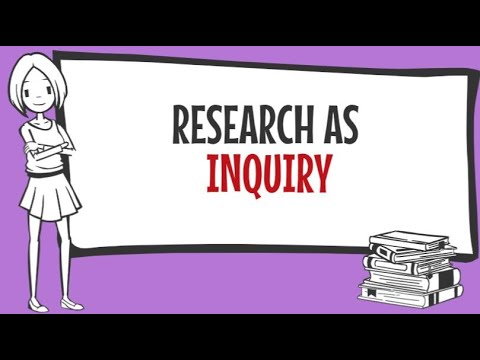
\includegraphics[keepaspectratio]{assets/u1/image1.jpeg}}

}

\end{figure}%

📖 \textbf{Read} Chapters 1 and 2 in in \emph{Introduction to Research
in Leadership} (Rosch et al., 2023).

✏️ Start a \textbf{Reflective Journal}. This journal is not submitted or
graded, but is an opportunity for you to reflect on, and engage with,
the course content. The questions posed will often help you prepare for
your assignments and are designed to help you successfully achieve the
learning outcomes for each unit.

Next, write about the following in your Reflective Journal:

\begin{itemize}
\tightlist
\item
  How would you define research?
\item
  Describe your experience with ``research.''

  \begin{itemize}
  \tightlist
  \item
    Have you taken an undergraduate statistics course?
  \item
    Is this your first time learning about research?
  \item
    Have you published your own scientific paper?
  \end{itemize}
\item
  How might relational approaches to inquiry change the way you frame
  research questions?
\item
  How can integrating ethical considerations into research contribute to
  leadership practices?
\end{itemize}

\textbf{Note:} Your Journal is not graded but will help you in your
assessment for this unit.

\subsection*{}\label{section}
\addcontentsline{toc}{subsection}{}

\bookmarksetup{startatroot}

\chapter*{Leadership and Scholarly
Inquiry}\label{leadership-and-scholarly-inquiry}
\addcontentsline{toc}{chapter}{Leadership and Scholarly Inquiry}

\markboth{Leadership and Scholarly Inquiry}{Leadership and Scholarly
Inquiry}

On what basis are sound decisions made? What evidence do leaders rely
upon for best outcomes? The need to evaluate evidence for best practices
in leadership decision-making is widely acknowledged. Patton (2001)
observes that ``the emphasis on knowledge generation disseminated in the
form of best practices has swept like wildfire through all sectors of
society'' (p.~329).

The MA in Leadership program emphasizes a vision of best practices in
leadership. What do is meant by this? Put simply, ``best practices''
refers to those practices and initiatives that result in the best
possible outcomes. What qualifies something as best practice?
Identifying best practices starts by understanding the common sources of
evidence available to leaders.

Take a moment to think about a recent decision you made as a leader. On
what did you base this decision? Previous experience? Values? Company
policy? Empirical evidence (e.g., data derived from research)? Expert
opinion? Systematic inquiry, as represented by research, is one tool
that leaders can use to inform best practices and their decision-making
process.

Systematic inquiry is hardly new; first century writings demonstrate
Bible evidence of systematic, logical, and empirical inquiry.

Consider the following passage from Luke, a physician trained in
empirical methods of his day:

\begin{quote}
Many have undertaken to draw up an account of the things that have been
fulfilled among us, just as they were handed down to us by those who
from the first were eyewitnesses and servants of the word. With this in
mind, since I myself have carefully investigated everything from the
beginning, I too decided to write an orderly account for you, most
excellent Theophilus, so that you may know the certainty of the things
you have been taught. (Luke 1:1-4, NIV)
\end{quote}

How does the research process differ from managerial activities such as
decision-making and problem solving? Research shares with
decision-making and problem-solving the systematic and disciplined
procedure of identifying an issue or problem, deciding on an approach,
formulating a plan, collecting and analyzing data, drawing conclusions,
and implementing decisions based on this rigorous process. What
distinguishes research from generic or everyday problem solving is its
commitment to advance or generate knowledge that typically will be
communicated to the larger academic or scientific community. Since the
beginning of the 21st century, there has been remarkable growth in the
foundations of research and research methodologies across the natural,
applied, and social sciences, as well as the humanities.

\section*{Boyer's Model of
Scholarship}\label{boyers-model-of-scholarship}
\addcontentsline{toc}{section}{Boyer's Model of Scholarship}

\markright{Boyer's Model of Scholarship}

The MA in Leadership program is focused on applied scholarship. In
defining this, Boyer's four-part Model of Scholarship (1997) is useful.
Boyer's typology identifies four domains of scholarship: discovery,
integration, application, and teaching. Marta Nibert (2011) discusses
the model in her paper titled ``Boyer's Model of Scholarship.''

In the section titled ``Application,'' Nibert (2011) notes that the
scholarship of application:

\begin{quote}
focuses on using research findings and innovations to remedy societal
problems. Included in this category are service activities that are
specifically tied to one's field of knowledge and professional
activities. Beneficiaries of these activities include commercial
entities, non-profit organizations, and professional associations (para.
4).
\end{quote}

Though Nibert's primary audience is the professoriate, this material is
relevant for MA Leadership learners. Application is highlighted because
this program was designed to focus on the scholarship of application,
although work in the capstone will likely include one or more of the
other domains.

\subsection*{Scholarship of Discovery}\label{scholarship-of-discovery}
\addcontentsline{toc}{subsection}{Scholarship of Discovery}

Boyer's Scholarship of Discovery is the type of scholarship associated
with traditional scholarly research. ``Research is a systematic process
of collecting, analyzing and interpreting information (data) in order to
increase our understanding of a phenomenon abut which we are interested
or concerned'' (Leedy \& Ormrod, 2010, p.~2). Boyer's Scholarship of
Discovery is often referred to as primary research\textbf{.} Primary
research is narrowly focused and contributes to the body of knowledge by
helping people understand one isolated part of reality in detail in the
hopes that this understanding can be generalized to a broader part of
reality. In traditional research, the Scholarship of Discovery falls
into two distinct genres: quantitative and qualitative research. Each of
these genres manifest in numerous variations, including hybrid models
involving both quantitative and qualitative elements, designed for and
suited to differing research questions.

\subsection*{Scholarship of
Integration}\label{scholarship-of-integration}
\addcontentsline{toc}{subsection}{Scholarship of Integration}

Boyer's Scholarship of Integration is ``the attempt to arrange relevant
bits of knowledge and insight from different disciplines into broader
patterns that reflect the actual interconnectedness of the world''
(Boyer, as cited in Jacobsen \& Jacobsen, 2004, p.~51).

The Scholarship of Integration often involves interdisciplinary
collaboration and requires critical analysis and review of knowledge,
followed by the creative synthesis of ideas to address specific topics
or issues.

\subsection*{Scholarship of
Application}\label{scholarship-of-application}
\addcontentsline{toc}{subsection}{Scholarship of Application}

The Scholarship of Application is ``the scholarship of engagement;
seeking to close the gap between values in the academy and the needs of
the larger world'' (Boyer, as cited in Jacobsen \& Jacobsen, 2004,
p.~51). In the Scholarship of Application, knowledge is applied to the
solution of societal needs and practice. In most cases, knowledge
stemming from the Scholarship of Discovery and the Scholarship of
Integration informs the solutions to problems. These scholarships are
often associated with the context of formal education. Although the
Scholarship of Application may happen within formal education contexts,
it is most often associated with other settings (Boshier, 2009, p.~6).

\subsection*{Scholarship of Teaching}\label{scholarship-of-teaching}
\addcontentsline{toc}{subsection}{Scholarship of Teaching}

Finally, the Scholarship of Teaching is ``the scholarship of sharing
knowledge'' (Boyer, as cited in Jacobsen \& Jacobsen, 2004, p.~51). The
Scholarship of Teaching involves the reflective analysis of the
knowledge about teaching and learning. This knowledge base itself is the
product of the Scholarships of Discovery, Integration and Application
combining as ``active ingredients of a dynamic and iterative teaching
process'' (Boshier, 2009, p.~5). Boyer's typology originally identified
as the Scholarship of Teaching has expanded and is now widely known in
literature as the Scholarship of Teaching and Learning (Boshier, 2009).

Boshier contends that Boyer's four domains were conceived holistically
as elements that overlap and interact, not as discrete elements,
appearing in any predictable order, and are better viewed as an
operating system than a list of discrete elements (Boshier, 2009,
pp.~4-5). As such, it is helpful to view the model as a Venn diagram
where each scholarship domain overlaps (see Figure 1).

\textbf{Figure 1}

Boyer's Model of Scholarship

\emph{Note:} This figure demonstrates how the four domains of Boyer's
Model of Scholarship overlap and interact to create a holistic system of
scholarship.

LDRS 591 is designed to help you understand types of research, identify
a research topic, develop a research question, and decide whether you
will pursue a thesis track in your MA Leadership studies. Should you
choose the thesis track, you will engage in Scholarship of Discovery,
meaning you will conduct primary research.

\textbf{Note:} Choosing the thesis track requires approval from the
Department of Leadership Program Director.

Most program students choose the capstone track, in which they conduct
secondary research.

\subsection*{Activity: Learning
Activity}\label{activity-learning-activity-1}
\addcontentsline{toc}{subsection}{Activity: Learning Activity}

📺 \textbf{Watch} the following video ``Introduction to Research
Design'' from
\href{https://www.youtube.com/@researchdoctoralse4565}{Research \&
Doctoral Services at Walden University} (2015) where Dr.~Patton
introduces the concept of research as a scholar-practitioner:

\begin{figure}[H]

\caption{https://img.youtube.com/vi/GYywR7SA03E/maxresdefault.jpg}

{\centering \pandocbounded{
\includegraphics[keepaspectratio]{assets/u1/image2.jpeg}}

}

\end{figure}%

✏️ \textbf{Respond} to the following in your Reflective Journal:

\begin{itemize}
\tightlist
\item
  Describe at least one example of a decision you have made as a leader.
\item
  Consider the factors that went into that decision making process
  (e.g., values, research, policy, past experience, expert opinion).
\item
  What do you consider as ``evidence'' in your decision making?
\item
  In your own words, why is evidence-based decision-making important in
  leadership?
\end{itemize}

\textbf{Note:} your Journal is not graded but will help you in your
assessment for this unit.

\bookmarksetup{startatroot}

\chapter*{Philosophical Foundations of
Research}\label{philosophical-foundations-of-research}
\addcontentsline{toc}{chapter}{Philosophical Foundations of Research}

\markboth{Philosophical Foundations of Research}{Philosophical
Foundations of Research}

A professor once observed that a fundamental attribute of being human is
the tendency to ask questions. Humanity is especially interested in
three fundamental questions:

\begin{itemize}
\tightlist
\item
  What is real?
\item
  What is true?
\item
  What is good?
\end{itemize}

The philosophical category of metaphysics is concerned with what is
real, and what is the nature of reality. The philosophical category of
epistemology is concerned with the truth, and the nature and process of
knowing. The philosophical category of axiology is concerned with what
is good and how people can determine the nature of goodness. Much of
history is a chronicle of the different ways people have answered these
three fundamental questions. How people answer these questions reveals
their perspective and worldview.

Every person bases their own thoughts, decisions, and actions on what is
called a worldview. A worldview is ``an interpretive framework through
which one makes sense of themselves, other people, and the world around
them'' (Geisler \& Watkins, 2003). It is like a pair of glasses that you
wear when you are observing things about yourself, other people, and the
world in which you live.

📺 \textbf{Watch} the following short video ``What's Your Worldview?
(Quiz)'' by the
\href{https://www.youtube.com/@Impact360instituteOrg}{Impact 360
Institute} (2015) that explains the concept of worldview:

\begin{figure}[H]

\caption{https://img.youtube.com/vi/VXnSE0uvwzM/maxresdefault.jpg}

{\centering \pandocbounded{
\includegraphics[keepaspectratio]{assets/u1/image3.jpeg}}

}

\end{figure}%

A discussion about worldview, or your perspective, is foundational to
what you want to accomplish in this course.

Throughout this course you will continuously consider:

\begin{enumerate}
\def\labelenumi{\arabic{enumi}.}
\tightlist
\item
  On what basis are sound decisions made?
\item
  What evidence do leaders rely upon for best outcomes when they are
  making decisions?
\end{enumerate}

Each person has a preference for obtaining truth or a framework for
understanding ourselves, others, and the world, and personal preferences
abound. Researchers and consumers of research approach knowledge,
learning, and life with a particular perspective. Understanding that
perspective is essential before beginning the research journey and is
especially important in leadership roles.

Figure 1. Research Paradigms (Springer, 2019)

\pandocbounded{\includegraphics[keepaspectratio]{assets/u1/image4.gif}}

\textbf{Source}:
\url{https://link.springer.com/article/10.1007/s40670-019-00898-9}

📺 \textbf{Watch} the following helpful video ``Ontology, Epistemology,
Methodology and Methods in Research Simplified!'' by
\href{https://www.youtube.com/@NurseKillam}{Laura Killam} (2015) that
explains Paradigms, Ontology and Epistemology:

\begin{figure}[H]

\caption{https://img.youtube.com/vi/hCOsY5rkRs8/maxresdefault.jpg}

{\centering \pandocbounded{
\includegraphics[keepaspectratio]{assets/u1/image5.jpeg}}

}

\end{figure}%

It is important to be aware of your worldview before you enter the
research journey because it will inform the types of questions that you
ask and the processes that you use to find the answers to your
questions.

As an example, review this Christian worldview and explore how it can be
applied to the research journey:

A Christian worldview asserts that God has created the world and
everything in it, and that truth is arrived at through a study of God's
specific revelation (the Bible) and general revelation (creation).
Christians believe not only in studying and understanding truth, but
they also believe in a personal God that has revealed Himself through
this created world.

The Christian worldview can be summarized in three words: Creation,
Fall, and Redemption. Consider what these terms mean in the context of
worldview. Initially, when God created the world, it was all good,
whole, and harmonious. God created man in His own image. Originally man
was created healthy in body, soul, and spirit (Genesis 1:26-27, 31). As
people rebelled against God, causing the Fall, the presence of sin
corrupted all aspects of God's good creation, and brought about much
suffering. Where there was formerly harmony and wholeness, we now
experience ourselves, our relationships, and the world around us as
fractured, broken, and full of dis-ease (a literal discomfort with who
we are) (Genesis 3).

Despite the brokenness, Christians believe that God is actively working
to bring about restoration and wholeness to His entire creation. Through
Christ's redemptive work on the cross, people are reconciled to God and
are challenged to make all things as they were created and meant to
be--very good. Redemption means that all things are made new in Christ
(Colossians 1:19-20).

The framework of Creation, Fall, and Redemption is important because it
allows people to enter a discussion about research with confidence
knowing that God's redemptive work touches this area. Christians believe
that we are called to study creation with the desire to take the
knowledge we gain and use it to help and bless others; to work toward
the restoration and healing of God's creation. Christians are called to
inquire, investigate, and ask questions, always with a view to serve
others.

Another example of a worldview is an Indigenous worldview, which grounds
reality, truth, and goodness in relational and interconnected terms. For
example, drawing from Battiste (2005) and Menzies (2001), Indigenous
philosophies often emphasize that reality is inherently interconnected
and inseparable from the land, community, and spirituality
(metaphysics). This relational understanding challenges individualistic
approaches to research. Further, Indigenous ways of knowing prioritize
collective experience, oral traditions, and lived knowledge passed down
through generations (epistemology). Knowledge is not only ``discovered''
but also co-created and shared with respect to its cultural and
environmental context. Finally, from an Indigenous perspective, what is
``good'' is often framed as what sustains harmony and well-being within
the community and environment, making ethics a central consideration in
the research process (axiology).

As Menzies (2001) explains, incorporating Indigenous perspectives into
research requires rethinking the researcher's role, emphasizing
reciprocity, mutual respect, and the co-creation of knowledge with the
communities involved.

\textbf{Note:} It is beyond the purpose of this course to go deeper into
this topic other than to make the point that our way of knowing and
understanding the world around you---your worldview---influences how you
approach all of life, including how you approach research and how you
use research to inform your decision-making process.

\subsection*{Activity: Learning
Activity}\label{activity-learning-activity-2}
\addcontentsline{toc}{subsection}{Activity: Learning Activity}

📺 \textbf{Watch} the following video where
\href{https://www.youtube.com/@garygramenz}{Gary Gramenz} (2014)
explains ``Philosophical Foundations for Research Methodology'':

\begin{figure}[H]

\caption{https://img.youtube.com/vi/j758XBXD4r4/maxresdefault.jpg}

{\centering \pandocbounded{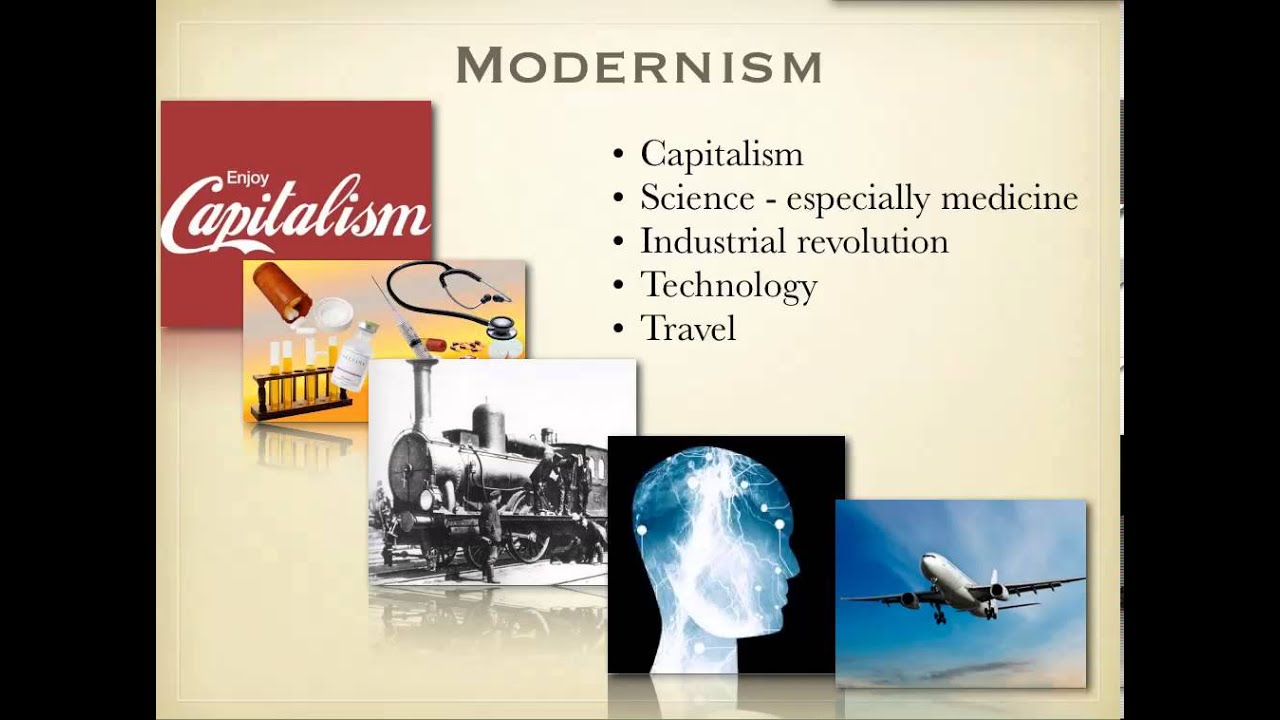
\includegraphics[keepaspectratio]{assets/u1/image6.jpeg}}

}

\end{figure}%

📖 \textbf{Read}
``\href{https://www.regent.edu/acad/global/publications/ijls/new/vol2iss2/Wallace/WallaceV2Is2.pdf}{Servant
Leadership: A Worldview Perspective}'' (Wallace, 2007).

📖 \textbf{Read}
``\href{https://www.researchgate.net/publication/338202096_A_Medical_Science_Educator\%27s_Guide_to_Selecting_a_Research_Paradigm_Building_a_Basis_for_Better_Research}{A
Medical Science Educator's Guide to Selecting a Research Paradigm:
Building a Basis for Better Research}'' (Brown \& Dueñas, 2020).

✏️ \textbf{Reflect} on your own worldview. Then answer the following in
your Reflective Journal:

\begin{itemize}
\tightlist
\item
  What motivates you? What are you driven by? (e.g.~funding, social
  justice, the common good)
\item
  Do you believe there is ``one verifiable reality,'' or that ``multiple
  socially constructed realities'' exist?
\item
  In what ways can your research contribute to the well-being of the
  communities you are studying?
\item
  What do you think counts as knowledge within the world?
\item
  How do you think knowledge is acquired?
\item
  Based on the Brown and Duenas article, what research paradigm
  resonates with you the most? (i.e., positivist, post-positivist,
  social constructivist, critical theory). Why does it resonate with
  you?
\end{itemize}

\textbf{Note:} your Journal is not graded but will help you in your
assessment for this unit.

\section*{Summary}\label{summary}
\addcontentsline{toc}{section}{Summary}

\markright{Summary}

In this unit you learned about what scholarly inquiry is, how to become
a scholarship practitioner, and what a worldview is. You also learned
about the importance of scholarly inquiry for leadership, the
implications of evidence-based decision making for leaders. In Unit 2,
you will learn about types of scholarly research.

\section*{Checking Your Learning}\label{checking-your-learning}
\addcontentsline{toc}{section}{Checking Your Learning}

\markright{Checking Your Learning}

Now that you completed the learning activities and assignments for this
unit, check the list below to ensure you can do the following:

\begin{enumerate}
\def\labelenumi{\arabic{enumi}.}
\tightlist
\item
  Can you distinguish between informal research and scholarly inquiry?
\item
  Can you discuss how scholarly inquiry applies to everyday decision
  making?
\item
  Reflect on why evidence-based decision making is important for
  leadership?
\end{enumerate}

Review the unit topics more in depth as needed or continue to the next
unit.

\section*{References}\label{references}
\addcontentsline{toc}{section}{References}

\markright{References}

\begin{quote}
Battiste, M. (2005). Indigenous knowledge: Foundations for First
Nations. \emph{WINHEC: International Journal of Indigenous Education
Scholarship}, \emph{1,} 1-17.
\url{https://journals.uvic.ca/index.php/winhec/article/view/19251.}

Boshier, R. (2009). Why is the scholarship of teaching and learning such
a hard sell? \emph{Higher Education Research and Development},
\emph{28}(1), 1-15.

Geisler, N., \& Watkins, W. D. (2003). \emph{Worlds apart: A handbook on
world views} (2nd ed.). Wipf and Stock.

Jacobsen, D., \& Jacobsen, R. (2004). \emph{Scholarship and Christian
faith: Enlarging the conversation}. Oxford University Press.

Leedy, P., \& Ormrod, J. (2010). \emph{Practical research: Planning and
design} (9th ed.). Pearson.

Menzies, C. R. (2001). \emph{Reflections on research with, for, and
among Indigenous peoples.} \emph{Open Journal Systems,
25}(1).https://doi.org/10.14288/cjne.v25i1.195900.

Nibert, M. (n.d.). \emph{Boyer's model of scholarship.} Expectations of
Faculty in Higher Education.
\url{https://www.facultyguidebook.com/BoyerModel.pdf.}

Patton, M. (2001). \emph{Qualitative research and evaluation methods}.
Sage.

Penner, D. (2017). INQUIRY 1SS3: Inquiry in the social sciences
{[}Syllabus{]}. McMaster University. Retrieved from
\url{https://facsocsci.mcmaster.ca/courses/inquiry-thinking-and-research-skills/fall-2022-socsci-2ss3-c02-penner/\%40\%40display-file/outline_file/SOCSCI\%25202SS3\%2520C02\%2520Penner\%2520Fall\%25202022.pdf.}

Plano-Clark, V., \& Creswell, J. (2015). \emph{Understanding research: A
consumer's guide} (2nd ed.). Pearson.

Rosch, D. M., Kniffin, L. E., \& Guthrie, K. L. (2023).
\emph{Introduction to research in leadership}. Information Age
Publishing.
\end{quote}

\bookmarksetup{startatroot}

\chapter*{Overview}\label{overview-1}
\addcontentsline{toc}{chapter}{Overview}

\markboth{Overview}{Overview}

Before you can effectively critique scholarly research, it is essential
to first understand what scholarly literature is and why it matters. In
graduate-level leadership studies, being able to engage with research
critically is not just an academic exercise, but a vital leadership
skill. Leaders must be able to evaluate research-based evidence, apply
it thoughtfully in practice, and contribute to informed decision-making
in their organizations and communities.

In this unit, you will be introduced to several common research
methodologies that are frequently used in leadership and social sciences
research:

\begin{itemize}
\tightlist
\item
  Quantitative Research
\item
  Qualitative Research
\item
  Mixed Methods Research
\item
  Literature Reviews
\item
  Systematic Literature Reviews
\item
  Scoping Reviews
\end{itemize}

Understanding these research approaches will equip you to read academic
studies with greater confidence, recognize the strengths and limitations
of different methodologies, and assess the credibility of research
findings. This knowledge is also essential for your upcoming
assignments, particularly your systematic literature review, which is a
major project in LDRS 697 and 698. Through this unit, you will begin
building the foundational skills necessary to complete that review, as
well as to become a more informed consumer of research throughout your
leadership practice.

\subsection*{Topics}\label{topics-1}
\addcontentsline{toc}{subsection}{Topics}

Unit 2 is divided into six topics. See the
\href{https://learn.twu.ca/mod/book/view.php?id=1172206}{\textbf{Unit 2
Topics}} link at the bottom of this page for the course notes on the
following topics:

\begin{enumerate}
\def\labelenumi{\arabic{enumi}.}
\tightlist
\item
  Introduction to Quantitative Research
\item
  Introduction to Qualitative Research Design
\item
  Introduction to Mixed Methods
\item
  Introduction to Literature Review vs.~Systematic Literature Review
\item
  Introduction to Scoping Review
\item
  Unit Summary
\end{enumerate}

\section*{Unit Outcomes}\label{unit-outcomes-1}
\addcontentsline{toc}{section}{Unit Outcomes}

\markright{Unit Outcomes}

When you have completed this unit, you should be able to:

\begin{enumerate}
\def\labelenumi{\arabic{enumi}.}
\tightlist
\item
  Describe the differences between a quantitative, qualitative, and
  mixed methods research report.
\item
  Identify the key differences between traditional literature reviews
  and systematic literature reviews, including their purposes and
  methodologies.
\item
  Explain the purpose of conducting a scoping review and how it can
  inform the development of research questions.
\end{enumerate}

\section*{Learning Activities}\label{learning-activities-1}
\addcontentsline{toc}{section}{Learning Activities}

\markright{Learning Activities}

Here is a checklist of learning activities you will benefit from in
completing this unit. You may find it useful for planning your work:

\begin{itemize}
\tightlist
\item
  Watch the video: ``Qualitative \& Quantitative Research--An
  Introduction.''
\item
  Read Chapters 5-10 and 12 in \emph{Introduction to Research in
  Leadership} (Rosch et al., 2023).
\item
  Choose a peer reviewed article about transformational servant
  leadership. Review the article and identify the research methodology
  used.
\end{itemize}

\subsection*{Resources}\label{resources-1}
\addcontentsline{toc}{subsection}{Resources}

Here are the resources you will need to complete this unit:

\begin{itemize}
\tightlist
\item
  Rosch, D. M., Kniffin, L. E., \& Guthrie, K. L. (2023).
  \emph{Introduction to research in leadership}. Information Age
  Publishing.
\item
  The articles in this unit can be found through the
  \href{https://www.twu.ca/academics/library}{TWU library}.
\end{itemize}

\bookmarksetup{startatroot}

\chapter*{Quantitative Research}\label{quantitative-research}
\addcontentsline{toc}{chapter}{Quantitative Research}

\markboth{Quantitative Research}{Quantitative Research}

The purpose of reviewing these materials is to become informed consumers
of research, rather than to develop expertise as researchers. This unit
gives a brief introduction to the quantitative and qualitative research
methodologies.

Plano-Clark and Creswell (2015) assert that quantitative and qualitative
research approaches are suited to various kinds of research questions: a
quantitative research approach is indicated when the research problem
requires explanation\textbf{,} while a qualitative research approach is
indicated when the research problem requires exploration\textbf{.}

From a Christian perspective, becoming an informed consumer of research
is deeply connected to the biblical call to seek truth, act justly, and
serve others. Research is not merely a technical exercise or a pursuit
of knowledge for its own sake; it is a means to align our actions and
understanding with God's purposes. Colossians 3:23 states, ``Whatever
you do, work heartily, as for the Lord and not for men,'' and reminds
people that diligence and integrity in all tasks, including engaging
with research, are forms of worship and service to God.

To be an informed consumer of research from a Christian perspective
means approaching inquiry with humility, recognizing that all truth
ultimately comes from God---John 14:6: ``I am the way, the truth, and
the life.'' This perspective calls people to critically evaluate the
methodologies, assumptions, and conclusions of research, ensuring they
align with ethical principles and the pursuit of justice (``To act
justly and to love mercy and to walk humbly with your God,'' Micah 6:8.)
For instance, quantitative methods may help you uncover patterns that
inform fair policies, while qualitative methods allow you to listen
deeply to the voices of traditionally marginalized individuals.

Additionally, research can be viewed as an act of stewardship, in which
people responsibly use the knowledge, resources, and abilities God has
entrusted to them to benefit others and bring glory to Him (``Each of
you should use whatever gift you have received to serve others, as
faithful stewards of God's grace in its various forms.'' 1 Peter 4:10.)
Engaging with research critically and ethically ensures that your
efforts do not exploit or harm but instead contribute to human
flourishing and the common good.

Finally, becoming an informed consumer of research also requires
discernment. Christians are called to weigh information carefully and
assess its validity (``But test everything; hold fast what is good,'' 1
Thessalonians 5:21) This discernment helps people navigate biases,
incomplete evidence, or conclusions that may conflict with Christian
values. By doing so, you uphold the integrity of our faith while
embracing research as a tool to seek knowledge, promote justice, and
serve God's purposes in the world. This commitment to discernment
extends beyond personal reflection and academic study. It also plays a
crucial role in leadership, where decisions often have significant
impacts on others. Leaders are called to apply the same thoughtful
evaluation to the research they use in their professional roles.

Leaders often face complex situations that require thoughtful decisions
grounded in credible evidence. For example, in an educational leadership
context, a school principal may review research on different
instructional models to determine which approach improves student
engagement and achievement. By carefully evaluating the research methods
and findings, the principal can select strategies that are both
evidence-based and appropriate for the school's unique community and
goals. This ability to assess and apply research ensures that leadership
decisions are thoughtful, ethical, and effective.

Learning to evaluate research equips you to make well-informed choices,
apply findings responsibly in your organization, and lead with integrity
and confidence. This skill will support you throughout this course and
in your leadership practice, particularly as you work toward completing
your systematic literature review project.

\bookmarksetup{startatroot}

\chapter*{Quantitative Methodology}\label{quantitative-methodology}
\addcontentsline{toc}{chapter}{Quantitative Methodology}

\markboth{Quantitative Methodology}{Quantitative Methodology}

Leedy and Ormrod (2010) assert that quantitative research has three
purposes: to explain and predict, to confirm and validate, and to test
theory. Rosch et al (2023) stated quantitative research is a process of
describing relationships with numbers: ``The central presumption of
quantitative research is that concepts can be represented by numbers''
(Rosch et al., 2023, p.~81).

According to Rosch et al.~(2023), quantitative research is a structured
method of inquiry that emphasizes measurement and analysis of numerical
data to understand relationships, behaviors, and outcomes. Further,
quantitative research is an approach that seeks to establish patterns
and test hypotheses through rigorous statistical techniques.
Quantitative research often begins with a clear hypothesis derived from
theory or prior research. Further, quantitative research uses
statistical tools to interpret data and validate hypotheses. Hypotheses
are evaluated through methods such as surveys or experiments. For
example, structured surveys can yield quantifiable data that researchers
analyze to draw conclusions about leadership effectiveness or
organizational dynamics (Rosch et al., 2023).

Quantitative research aligns with the Christian commitment to
stewardship and truth-seeking. The Bible emphasizes the importance of
seeking understanding and using it wisely---Proverbs 2:6: ``For the Lord
gives wisdom; from his mouth come knowledge and understanding.''.
Researchers are encouraged to approach data analysis with integrity,
ensuring that their work serves the greater good and aligns with ethical
principles that prioritize the well-being of others.

In summary, quantitative research is a vital approach in the study of
leadership, offering a systematic way to collect and analyze data, test
theories, and derive insights that can inform leadership practices and
strategies. Through structured methodologies and statistical rigor, it
provides a foundation for understanding complex relationships and
informing decision-making.

\bookmarksetup{startatroot}

\chapter*{Qualitative Research}\label{qualitative-research}
\addcontentsline{toc}{chapter}{Qualitative Research}

\markboth{Qualitative Research}{Qualitative Research}

\section*{Qualitative Methodology}\label{qualitative-methodology}
\addcontentsline{toc}{section}{Qualitative Methodology}

\markright{Qualitative Methodology}

In contrast to quantitative research, qualitative research has three
distinct purposes: to describe and explain, to explore and interpret,
and to build theory (Leedy \& Ormrod, 2010). These differing research
purposes find expression in differing research processes, the kinds of
data gathered, the approaches to data analysis, and finally in the ways
findings are communicated.

Counter to quantitative research, qualitative research is a method of
inquiry that focuses on understanding complex phenomena through the
collection and analysis of non-numerical data, such as words, images,
and experiences. In Chapter 8 of \emph{Introduction to Research in
Leadership}, Rosch et al.~(2023) describe qualitative research as an
approach that seeks to explore the depth and richness of human
experience, particularly in social and organizational contexts.

Because qualitative research focuses on human experiences, it resonates
strongly with Indigenous approaches to knowledge, which prioritize
relationships, context, and interconnectedness. Menzies (2001)
emphasized that Indigenous methodologies often involve storytelling,
oral traditions, and respect for the lived experiences of participants.
Researchers are encouraged to adopt a relational approach, viewing
participants as co-creators of knowledge rather than subjects of study.
This perspective ensures that research benefits the community and the
academic field, embodying principles of reciprocity and respect.

To explore human experiences, qualitative research often involves
conducting interviews, focus groups, or content analysis, which allow
researchers to gather insights into participants' perspectives,
experiences, motivations, and emotions. Qualitative research is
particularly valuable in leadership studies, as it captures the nuances
of individual and group dynamics that quantitative methods might
overlook.

Additionally, a key feature of qualitative research is its flexibility;
researchers can adapt their methods as new insights emerge during the
study. Rosch et al.~(2023) note that this adaptability enables a deeper
understanding of the context in which leadership occurs. The authors
also highlight the importance of reflexivity, encouraging researchers to
reflect on their own biases and influences throughout the research
process.

In summary, qualitative research provides a rich and detailed
understanding of human behavior and organizational phenomena, making it
an essential tool for exploring the complexities of leadership and
decision-making.

The differing designs of quantitative and qualitative research lead to
marked differences in how data are analyzed. Quantitative data is
approached primarily through deductive reasoning, employing statistical
analyses applied to numerical data, with stress on objectivity. In
contrast, qualitative data is approached primarily through inductive
reasoning with the goal being to uncover themes and categories, with
acknowledgement of potential researcher bias and subjectivity.
Typically, quantitative research findings are reported in a formal,
scientific style with full display of numbers and statistics, while
qualitative research findings are typically reported in a narrative form
(Leedy \& Ormrod, 2010). Table 2.1 shows the similarities and difference
between quantitative and qualitative research.

\textbf{Table 2.1. Comparison of Quantitative and Qualitative Research
Approaches}

Quantitative

Qualitative

General framework

Seek to confirm hypotheses about phenomena Instruments use more rigid
style of eliciting and categorizing responses to questions Use highly
structured methods such as questionnaires, surveys, and structured
observation

Seek to explore phenomena Instruments use more flexible, iterative style
of eliciting and categorizing responses to questions Use semi-structured
methods such as in-depth interviews, focus groups, and participant
observation

Analytical objectives

To quantify variation To predict causal relationships To describe
characteristics of a population

To describe variation To describe and explain relationships To describe
individual experiences To describe group norms

Question format

Closed-ended

Open-ended

Data format

Numerical (obtained by assigning numerical values to responses)

Textual (obtained from visual artifacts, audiotapes, videotapes, and
field notes)

Flexibility in study design

Study design is stable from beginning to end Participant responses do
not influence or determine how and which questions researchers ask next
Study design is subject to statistical assumptions and conditions

Some aspects of the study are flexible Participant responses affect how
and which questions researchers ask next Study design is iterative; data
collection and research questions are adjusted according to what is
learned

\emph{Qualitative Research Methods: A Data Collector's Field Guide}
(Woodsong et al., 2009).
\url{https://www.researchgate.net/publication/215666086_Qualitative_Research_Methods_A_Data_Collector’s_Field_Guide}

\bookmarksetup{startatroot}

\chapter*{Mixed Methods Research}\label{mixed-methods-research}
\addcontentsline{toc}{chapter}{Mixed Methods Research}

\markboth{Mixed Methods Research}{Mixed Methods Research}

\section*{Mixed Methods Methodology}\label{mixed-methods-methodology}
\addcontentsline{toc}{section}{Mixed Methods Methodology}

\markright{Mixed Methods Methodology}

Mixed methods research combines quantitative and qualitative approaches
to provide a comprehensive understanding of complex phenomena. Rosch et
al.~(2023) describe mixed methods as a strategy that leverages the
strengths of both methodologies, allowing researchers to explore
questions from multiple perspectives.

Mixed methods research involves collecting and analyzing both numerical
data and non-numerical data, which can enrich the findings and offer
deeper insights. For example, researchers might use quantitative surveys
to identify trends and patterns, followed by qualitative interviews to
explore the meanings and experiences behind those trends. This approach
enhances the validity and reliability of the research, as it provides a
more holistic view of the subject matter (Rosch et al., 2023).

Mixed methods research reflects the biblical principle of seeking wisdom
through multiple sources (``Plans fail for lack of counsel, but with
many advisers, they succeed,'' Proverbs 15:22). Combining quantitative
and qualitative insights mirrors the Christian commitment to balance and
thorough understanding in addressing complex issues.

Rosch et al.~(2023) also highlight the importance of integrating the
findings from both methods to create a cohesive narrative that informs
leadership practices and theories. This reflects the biblical principle
of seeking wisdom through multiple sources, as Proverbs 15:22 states,
``Plans fail for lack of counsel, but with many advisers, they
succeed.'' Combining quantitative and qualitative insights mirrors the
Christian commitment to balance and thorough understanding in addressing
complex issues. By employing mixed methods, researchers can address
complex questions that cannot be fully understood through a single
methodological lens.

In summary, mixed methods research is a powerful approach in leadership
studies, facilitating a multifaceted exploration of issues and
contributing to a richer understanding of organizational dynamics and
human behavior.

\subsection*{Activity: Learning
Activity}\label{activity-learning-activity-3}
\addcontentsline{toc}{subsection}{Activity: Learning Activity}

📺 \textbf{Watch} the following videos:

\begin{itemize}
\tightlist
\item
  ``Qualitative \& Quantitative Research -- An Introduction'' by
  \href{https://www.youtube.com/@TineJuhl}{Tine Juhl} (2017).
\end{itemize}

\begin{quote}
\begin{figure}[H]

\caption{https://img.youtube.com/vi/RYmLE8UqCXU/0.jpg}

{\centering \pandocbounded{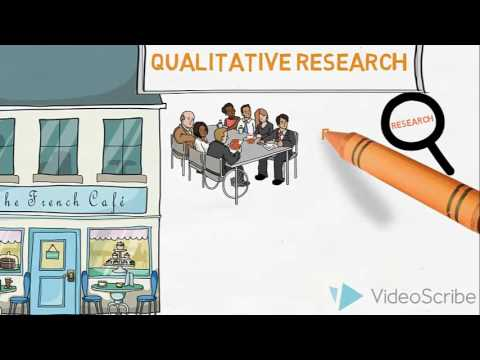
\includegraphics[keepaspectratio]{assets/u2/image1.jpeg}}

}

\end{figure}%
\end{quote}

\begin{itemize}
\tightlist
\item
  ``What is Mixed Methods Research?'' by
  \href{https://www.youtube.com/user/umhealthsystem/umhealthsystem}{Michigan
  Medicine} (2023).
\end{itemize}

\begin{figure}[H]

\caption{https://img.youtube.com/vi/1OaNiTlpyX8/maxresdefault.jpg}

{\centering \pandocbounded{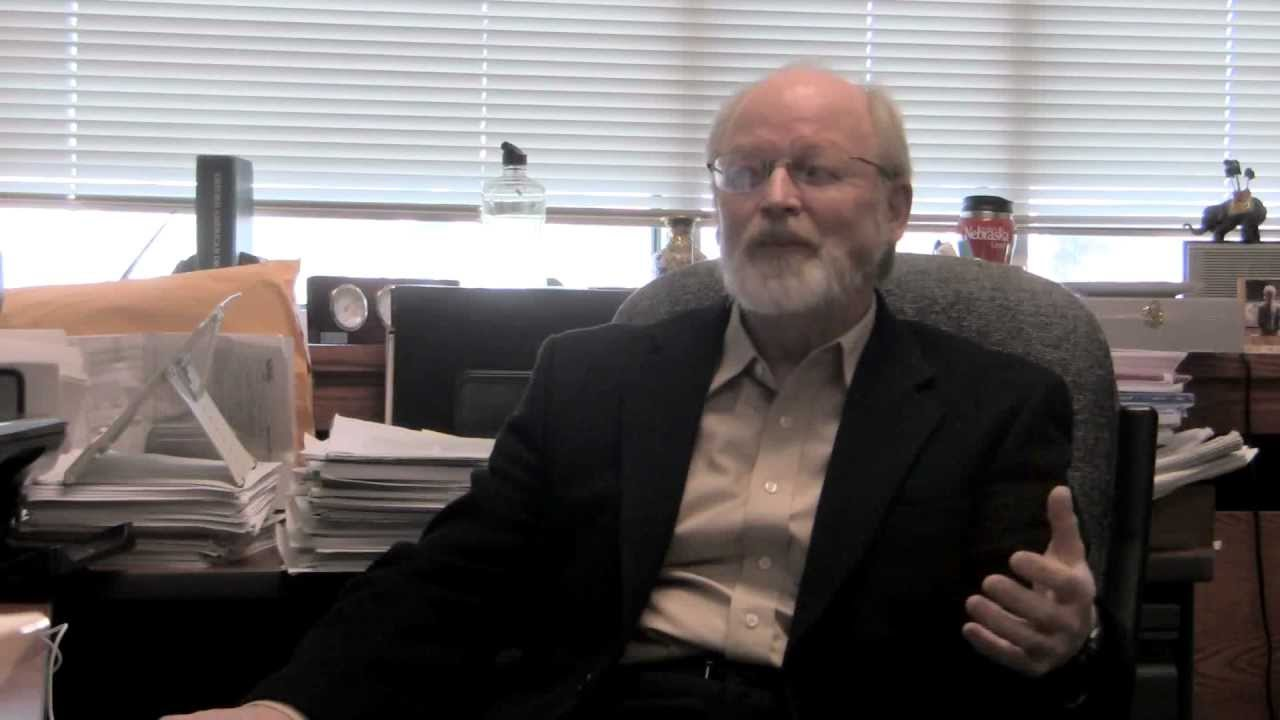
\includegraphics[keepaspectratio]{assets/u2/image2.jpeg}}

}

\end{figure}%

✏️ \textbf{Reflect.} After reading the chapters assigned, write about
the following in your Reflective Journal.

\begin{itemize}
\tightlist
\item
  Discuss the differences between qualitative, quantitative, and mixed
  methods research reports.
\item
  What are the potential challenges for studying servant leadership
  using a quantitative research approach?
\item
  From a Christian perspective, how can your research serve others and
  reflect ethical stewardship of knowledge?
\item
  How might Indigenous approaches to relational inquiry (e.g.,
  storytelling, community consultations) inform your understanding of
  qualitative research?
\end{itemize}

\textbf{Note:} Your Journal is not graded but will help you in your
assessment for this unit.

\subsection*{Activity: Identifying Research Methodologies in
Practice}\label{activity-identifying-research-methodologies-in-practice}
\addcontentsline{toc}{subsection}{Activity: Identifying Research
Methodologies in Practice}

\begin{enumerate}
\def\labelenumi{\arabic{enumi}.}
\tightlist
\item
  Read the following three articles:

  \begin{itemize}
  \tightlist
  \item
    \textbf{Qualitative Article:} Canavesi \& Martini (2021) --
    \href{https://mytwu-my.sharepoint.com/personal/jodi_mcbride_twu_ca/Documents/Documents/591\%20Curriculum\%20Revision/Articles/Canavesi\%20SL\%20Qualitative.pdf}{Spirituality
    and leader--follower relationships}
  \item
    \textbf{Quantitative Article:} Murari \& Gupta (2012) --
    \href{https://mytwu-my.sharepoint.com/personal/jodi_mcbride_twu_ca/Documents/Documents/591\%20Curriculum\%20Revision/Articles/Gupta\%20Quant.pdf}{Impact
    of Servant Leadership on Employee Empowerment}
  \item
    \textbf{Mixed-Methods Article:} Kendall (2025)
    \href{https://mytwu-my.sharepoint.com/personal/jodi_mcbride_twu_ca/Documents/Documents/591\%20Curriculum\%20Revision/Articles/Kendall\%20mixed\%20methods\%20nursing.pdf}{--
    Exploring gameplay to support leadership skills in nursing}
  \end{itemize}
\item
  Complete the chart below for each article. Be ready to explain how you
  determined the methodology used.
  \href{https://mytwu-my.sharepoint.com/personal/jodi_mcbride_twu_ca/Documents/Documents/591\%20Curriculum\%20Revision/New\%20Support\%20Documents/Unit\%202\%20ID\%20types\%20of\%20research\%20learning\%20actvity\%20chart.docx}{Click
  here for a Word template of the chart}.
\end{enumerate}

\subsubsection*{Comparison Chart}\label{comparison-chart}
\addcontentsline{toc}{subsubsection}{Comparison Chart}

\begin{longtable}[]{@{}
  >{\raggedright\arraybackslash}p{(\linewidth - 6\tabcolsep) * \real{0.4722}}
  >{\raggedright\arraybackslash}p{(\linewidth - 6\tabcolsep) * \real{0.2083}}
  >{\raggedright\arraybackslash}p{(\linewidth - 6\tabcolsep) * \real{0.1806}}
  >{\raggedright\arraybackslash}p{(\linewidth - 6\tabcolsep) * \real{0.1389}}@{}}
\toprule\noalign{}
\begin{minipage}[b]{\linewidth}\raggedright
\textbf{Criteria}
\end{minipage} & \begin{minipage}[b]{\linewidth}\raggedright
\textbf{Canavesi \& Martini (2021)}
\end{minipage} & \begin{minipage}[b]{\linewidth}\raggedright
\textbf{Murari \& Gupta (2012)}
\end{minipage} & \begin{minipage}[b]{\linewidth}\raggedright
\textbf{Kendall (2025)}
\end{minipage} \\
\midrule\noalign{}
\endhead
\bottomrule\noalign{}
\endlastfoot
\textbf{Research Purpose} & & & \\
\textbf{Primary Data Collection Method(s)} & & & \\
\textbf{Sample Size and Type} & & & \\
\textbf{Data Analysis Approach} & & & \\
\textbf{Language Cues (e.g., thematic, statistical)} & & & \\
\textbf{Declared Methodology} & & & \\
\textbf{Your Conclusion on Type of Study} (Qualitative / Quantitative /
Mixed) & & & \\
\end{longtable}

\subsubsection*{Reflection Questions}\label{reflection-questions}
\addcontentsline{toc}{subsubsection}{Reflection Questions}

\begin{itemize}
\tightlist
\item
  What features helped you identify the methodology?
\item
  How do the strengths and limitations of each approach show up in the
  findings?
\item
  Which method would be most appropriate for your own research
  interests? Why?
\end{itemize}

\bookmarksetup{startatroot}

\chapter*{Literature Reviews vs Systematic Literature
Reviews}\label{literature-reviews-vs-systematic-literature-reviews}
\addcontentsline{toc}{chapter}{Literature Reviews vs Systematic
Literature Reviews}

\markboth{Literature Reviews vs Systematic Literature
Reviews}{Literature Reviews vs Systematic Literature Reviews}

Literature reviews serve as foundational tools for understanding the
breadth and depth of existing research on a topic. They help scholars
identify gaps in knowledge, establish a framework for future inquiry,
and situate their work within broader academic conversations. This
section explores traditional literature reviews, systematic literature
reviews (SLRs), and scoping reviews, highlighting their differences and
uses.

\section*{Literature Review}\label{literature-review}
\addcontentsline{toc}{section}{Literature Review}

\markright{Literature Review}

Whether or not you realize it, you may have read literature reviews in
your studies to date.

By definition, a literature review examines and evaluates published work
related to a specific subject. In some cases, it focuses on research
from a particular time frame. Rather than simply summarizing sources, a
literature review follows a structured approach that blends summary with
synthesis. While a summary highlights the key points from each source,
synthesis involves reorganizing and integrating that information to
present new insights or connections among the studies (Mastrodonato,
n.d.).

Rosch et al.~(2023) highlight that a traditional literature review is
often narrative and subjective, summarizing existing research without
adhering to a strict methodology. Traditional reviews may lack
comprehensive search strategies and systematic analysis, leading to
potential biases in how studies are selected and interpreted.

Additionally, Cooper (1988) identified the primary functions of
literature reviews as summarising, classifying, and critically
evaluating, which help inform researchers about what has been done and
what remains to be explored about a particular topic.

Rosch et al.~(2023) emphasize that literature reviews play a crucial
role in research, particularly in fields like leadership, by offering
insights into theoretical frameworks, methodologies, and practical
implications. Literature reviews help researchers situate their work
within the broader academic discourse and can guide future research
directions.

Additionally, peer-reviewed studies consistently highlight the
importance of literature reviews in establishing a foundation for new
research by summarizing existing work, identifying gaps, and guiding
future inquiry (Cooper, 1988). Literature reviews play a crucial role in
research, particularly in fields like leadership, by offering insights
into theoretical frameworks, methodologies, and practical implications
(Rosch et al., 2023. This flexibility can lead to biases in how studies
are selected and interpreted, particularly when search strategies and
analyses are not comprehensive.

From a Christian perspective, engaging with literature reviews reflects
the biblical call to stewardship and the pursuit of truth. By
thoughtfully analyzing and synthesizing previous research, scholars
fulfill their responsibility to use knowledge wisely, align their work
with ethical principles, and serve the greater good---Colossians 3:23:
``Whatever you do, work heartily, as for the Lord and not for men.'' The
narrative nature of traditional literature reviews aligns with this
stewardship by encouraging researchers to thoughtfully engage with
existing knowledge while remaining diligent and accountable in their
efforts---Proverbs 21:5: ``The plans of the diligent lead surely to
abundance.''

Moreover, literature reviews can be understood as a form of
storytelling, resonating with Indigenous methodologies that value
relationality and interconnectedness (Battiste, 2005; Menzies, 2001).
For Indigenous scholars, storytelling is an essential practice for
weaving together diverse knowledge sources, preserving their integrity,
and situating them within a broader relational context. Traditional
literature reviews parallel this practice by connecting past knowledge
to current and future inquiry, ensuring that the voices and perspectives
within the research are acknowledged and respected.

\section*{Systematic Literature
Review}\label{systematic-literature-review}
\addcontentsline{toc}{section}{Systematic Literature Review}

\markright{Systematic Literature Review}

While traditional literature reviews provide a flexible narrative
overview, more structured approaches, such as systematic literature
reviews (SLRs), emphasize rigor and reproducibility.

A SLR is a comprehensive and structured approach to evaluating existing
research on a specific research question or topic. Unlike traditional
reviews, which provide a flexible narrative overview, SLRs emphasize
rigor, reproducibility, and the minimization of bias by adhering to
predefined protocols for search strategies and data synthesis (Rosch et
al., 2023). According to Cherry et al.~(2024), an SLR systematically
identifies, evaluates, and synthesizes research studies using a defined
protocol---which includes clear inclusion and exclusion criteria, a
thorough literature search, and systematic data extraction. This
structured process ensures that the review is transparent and
reproducible, offering reliable conclusions that guide future research.

These methods minimize bias by following predefined protocols for search
strategies and data synthesis, ensuring that the process is rigorous and
reliable (Rosch et al., 2023). This structured approach embodies
Christian values of diligence and integrity, reflecting the importance
of producing trustworthy research that serves others responsibly. As
Proverbs 25:2 states, ``It is the glory of God to conceal things, but
the glory of kings is to search things out,'' highlighting the biblical
principle of thoroughness and stewardship in the pursuit of knowledge.

This emphasis on diligence and intentionality finds a parallel in
Indigenous perspectives on knowledge. From an Indigenous worldview, the
careful and systematic nature of SLRs aligns with the respect and
intentionality required in honoring and preserving knowledge. Both
approaches value the ethical responsibility to ensure that information
is situated within its proper relational and cultural contexts. By
synthesizing information thoughtfully and respectfully, SLRs embody both
the precision of systematic inquiry and the relational ethics
foundational to Indigenous ways of knowing (Menzies, 2001).

While both traditional literature reviews and SLRs aim to synthesize
existing research, their methodologies and purposes differ
significantly. Traditional reviews offer a narrative and often
subjective overview of research, providing flexibility in summarizing
and critiquing studies without strict adherence to predefined protocols.
This approach allows for creative integration of diverse perspectives
but may introduce bias and limit reproducibility. In contrast, SLRs
employ a rigorous, structured methodology to minimize bias, ensure
transparency, and enhance reproducibility. By following predefined
protocols, including clear inclusion and exclusion criteria, systematic
data extraction, and comprehensive search strategies, SLRs provide
reliable and objective insights that guide future research. These
distinctions highlight the flexibility of traditional reviews for
exploratory work and the precision of SLRs for generating trustworthy
and reproducible findings. Both approaches play essential roles in
advancing scholarship when used appropriately within their respective
contexts.

Table 2.2 captures the key differences and similarities between
literature reviews and systematic literature reviews. Additionally,
\href{https://mytwu-my.sharepoint.com/personal/jodi_mcbride_twu_ca/Documents/Documents/697/A\%20Systematic\%20Literature\%20Review\%20of\%20Servant\%20Leadership\%20Theory\%20in\%20Organizational\%20Contexts.pdf}{click
here for a sample SLR}.

\textbf{Table 2.2 Differences between Literature Reviews and SLRs}

\begin{longtable}[]{@{}
  >{\raggedright\arraybackslash}p{(\linewidth - 4\tabcolsep) * \real{0.1667}}
  >{\raggedright\arraybackslash}p{(\linewidth - 4\tabcolsep) * \real{0.2917}}
  >{\raggedright\arraybackslash}p{(\linewidth - 4\tabcolsep) * \real{0.5417}}@{}}
\toprule\noalign{}
\begin{minipage}[b]{\linewidth}\raggedright
\textbf{Feature}
\end{minipage} & \begin{minipage}[b]{\linewidth}\raggedright
\textbf{Literature Review}
\end{minipage} & \begin{minipage}[b]{\linewidth}\raggedright
\textbf{Systematic Literature Review}
\end{minipage} \\
\midrule\noalign{}
\endhead
\bottomrule\noalign{}
\endlastfoot
\textbf{Purpose} & Summarizes existing research & Provides a
comprehensive and objective research synthesis \\
\textbf{Methodology} & Narrative and subjective & Structured,
reproducible, and systematic \\
\textbf{Search Strategy} & May be selective and not exhaustive &
Comprehensive and predefined search strategy \\
\textbf{Inclusion Criteria} & Often vague or informal & Clearly defined
and strictly applied \\
\textbf{Data Analysis} & Qualitative and descriptive & Quantitative and
qualitative synthesis \\
\textbf{Bias} & Higher potential for bias & Minimizes bias through
systematic protocols \\
\textbf{Outcome} & Provides context and identifies trends & Aims to
answer specific research questions with rigor \\
\textbf{Reproducibility} & Difficult to replicate & Designed to be
replicable \\
\end{longtable}

\section*{}\label{section-1}
\addcontentsline{toc}{section}{}

\markright{}

\section*{Scoping Review}\label{scoping-review}
\addcontentsline{toc}{section}{Scoping Review}

\markright{Scoping Review}

A scoping review is a preliminary assessment of the available literature
on a broad topic (Cherry et al., 2024). A scoping review, sometimes
called a scoping search, should be the first search you conduct, using
simple search terms to identify general literature relevant to your
topic.

More specifically, a scoping review is a distinct type of evidence
synthesis methodology that systematically identifies, evaluates, and
maps the breadth of knowledge on a specific topic or field. Unlike
traditional literature reviews or systematic literature reviews, scoping
reviews are not comprehensive and do not aim to answer a specific
research question. Instead, Cherry et al.~(2024) state they are
``performed to determine whether your topic area is suitable for a
review by giving you a snapshot of the volume and type of evidence
available'' (p.~45). To determine whether a topic is suitable for
researcher, scoping reviews systematically identify, evaluate, and map
the breadth of knowledge on a specific topic or field. Unlike systematic
reviews, which focus on answering narrowly defined research questions,
scoping reviews address broader questions to explore and describe the
extent and characteristics of existing literature (Sharma \& Goyal,
2023).

In summary, the goal of a scoping review is to:

\begin{enumerate}
\def\labelenumi{\arabic{enumi}.}
\tightlist
\item
  Understand the extent and type of research available on a topic.
\item
  Determine the relevance of a topic by evaluating the volume and
  diversity of existing evidence.
\item
  Identify trends, gaps, and areas for further study.
\end{enumerate}

Scoping reviews must be conducted early in your research, before
finalizing your research question. Doing so is useful in identifying
underexplored fields, where mapping the range and type of studies can
clarify concepts, identify gaps, and guide future research directions.

To ensure a transparent and reliable process, the following steps are
critical when conducting a scoping review:

\begin{enumerate}
\def\labelenumi{\arabic{enumi}.}
\tightlist
\item
  \textbf{Identify the Research Question} The research question is the
  cornerstone of a scoping review. It should be broad enough to capture
  the diversity of literature on the topic, yet clearly defined to
  maintain focus and direction. Using sub-questions can help balance the
  breadth of inquiry while ensuring the depth of analysis (Sharma \&
  Goyal, 2023).
\item
  \textbf{Identify Relevant Studies} Develop a comprehensive search
  strategy that specifies databases, search terms, and other
  sources---such as organizational websites and key references. This
  step ensures that the review includes diverse and interdisciplinary
  perspectives, drawing from published and unpublished literature
  (Sharma \& Goyal, 2023).
\item
  \textbf{Select Studies} Screen studies based on predefined inclusion
  and exclusion criteria. This process typically involves reviewing
  titles, abstracts, and full texts to determine relevance, where
  necessary. Employing multiple reviewers and using a flow diagram, as
  recommended by the PRISMA-ScR (Preferred Reporting Items for
  Systematic reviews and Meta-Analyses extension for Scoping Reviews)
  guidelines, enhances transparency and reproducibility (Sharma \&
  Goyal, 2023).
\item
  \textbf{Chart the Data} Extract and organize key information from each
  study in a systematic format, such as a spreadsheet or database.
  Categories often include the author, publication year, study location,
  population, methodology, main findings, and limitations. This
  structured approach facilitates a clear overview of the evidence
  (Sharma \& Goyal, 2023).
\item
  \textbf{Collate, Summarize, and Report Results} Synthesize findings
  into a narrative or descriptive summary that highlights the
  relationships between the evidence and the review objectives. Visual
  representations, such as tables, charts, or diagrams, can further
  illustrate the distribution and characteristics of the included
  studies (Sharma \& Goyal, 2023).
\item
  \textbf{Consult Stakeholders (Optional)} Engage with stakeholders,
  such as experts or practitioners, to refine the research question,
  validate findings, or provide feedback. This step enhances the
  relevance and practical application of the review, particularly for
  interdisciplinary or applied topics (Sharma \& Goyal, 2023).
\end{enumerate}

Scoping reviews provide a comprehensive and flexible method for
understanding the scope and characteristics of available evidence,
particularly in areas where research is heterogeneous or evolving. By
following these structured steps, researchers ensure their findings are
robust, transparent, and useful for informing future studies.
\href{https://mytwu-my.sharepoint.com/personal/jodi_mcbride_twu_ca/Documents/Documents/591\%20Curriculum\%20Revision/Articles/TESOL\%20Journal\%20-\%202025\%20-\%20Reinders\%20-\%20Conceptualizations\%20of\%20and\%20Research\%20on\%20Language\%20Teacher\%20Leadership\%20\%20A\%20Scoping\%20Review.pdf}{Click
here for a sample scoping review.}

This aligns with servant leadership principles by fostering informed
decision-making that serves the greater good and prioritizes others'
needs. From a Christian perspective, the diligence and intentionality
required in scoping reviews reflect the biblical call to seek truth and
apply knowledge in ways that glorify God and benefit the community
(Proverbs 3:13-14).

\subsection*{Activity: Learning
Activity}\label{activity-learning-activity-4}
\addcontentsline{toc}{subsection}{Activity: Learning Activity}

📺 \textbf{Watch} the following video
``\href{https://www.youtube.com/watch?app=desktop&si=jyp8a-827EYUC2HA&v=YVckIl8_ZCg&feature=youtu.be}{Systematic
vs.~Scoping Review: What's the Difference?}'' by
\href{https://www.youtube.com/@carrieprice78}{Carrie Prices} (2021).

📖 \textbf{Read} Chapters 5-10 and 12 in Introduction to Research in
Leadership (Rosch et al., 2023).

✏️\textbf{Respond} to the following in your Reflective Journal:

\begin{itemize}
\tightlist
\item
  Discuss the differences between literature reviews, scoping reviews,
  and systematic literature reviews.
\end{itemize}

\textbf{Note:} Your Journal is not graded but will help you in your
assessment for this unit.

\section*{Summary}\label{summary-1}
\addcontentsline{toc}{section}{Summary}

\markright{Summary}

In conclusion, the exploration of quantitative, qualitative, and mixed
methods research methodologies demonstrates the diverse approaches
researchers can take to address complex questions. Quantitative
research, with its emphasis on numerical analysis and structured
methods, provides a systematic framework for uncovering patterns,
validating theories, and explaining relationships (Leedy \& Ormrod,
2010; Rosch et al., 2023). This approach aligns with the Christian value
of stewardship, emphasizing diligence and integrity in managing and
interpreting data to serve the greater good.

Conversely, qualitative research offers rich insights into human
experiences and complex phenomena through methods like interviews and
observations. This approach captures the nuances of leadership and group
dynamics, resonating with Indigenous perspectives that value
relationality, storytelling, and the interconnectedness of knowledge
(Menzies, 2001; Rosch et al., 2023). By prioritizing relationships and
context, qualitative research fosters deeper understanding and
reciprocity, ensuring that inquiry benefits both researchers and
communities.

Mixed methods research integrates the strengths of both quantitative and
qualitative approaches, offering a holistic view of multifaceted issues.
This methodology reflects the Christian principle of seeking wisdom
through multiple sources---Proverbs 15:22: ``Plans fail for lack of
counsel, but with many advisers, they succeed.'' By combining diverse
perspectives, mixed methods research enhances the validity of findings
and supports comprehensive decision-making in leadership contexts (Rosch
et al., 2023).

The unit also highlighted the essential roles of literature reviews,
systematic literature reviews, and scoping reviews. Traditional
literature reviews provide narrative overviews, while SLRs emphasize
rigor and reproducibility through structured protocols that minimize
bias and ensure transparency (Cherry et al., 2024; Sharma \& Goyal,
2023). Scoping reviews, meanwhile, offer a broad assessment of available
evidence, helping researchers refine their focus and identify knowledge
gaps. These methodologies---when approached with respect for
relationality and intentionality---align with both Indigenous values of
honoring knowledge and Christian principles of stewardship and service.

As you develop as a consumer of research, understanding these
methodologies equips you to critically evaluate scholarly work, apply
evidence-based practices, and contribute to informed leadership. By
incorporating the principles of servant leadership, relational ethics,
and the pursuit of truth, researchers can ensure their work serves the
needs of their communities while advancing knowledge in meaningful and
impactful ways.

\section*{Checking Your Learning}\label{checking-your-learning-1}
\addcontentsline{toc}{section}{Checking Your Learning}

\markright{Checking Your Learning}

Now that you have completed the learning activities and assignments for
this unit, check the list below to ensure you can do the following:

\begin{enumerate}
\def\labelenumi{\arabic{enumi}.}
\tightlist
\item
  Can you describe the differences between a quantitative, qualitative,
  and mixed methods research report?
\item
  How can scoping reviews help researchers refine their research
  questions?
\item
  What are the main characteristics that differentiate a traditional
  literature review from a systematic literature review?
\item
  How does the methodological rigor of systematic literature reviews
  contribute to research transparency?
\item
  How can the principles of servant leadership guide researchers in
  applying the findings of a scoping or systematic review to serve the
  needs of their communities?
\item
  From a Christian or Indigenous perspective, how can respect for
  relationality and stewardship influence the way researchers approach
  literature reviews and evidence synthesis?
\end{enumerate}

\textbf{Review the unit topics more in depth as needed or continue to
the next unit.}

\section*{References}\label{references-1}
\addcontentsline{toc}{section}{References}

\markright{References}

Cherry, M. G., Boland, A., \& Dickson, R. (2023). \emph{Doing a
systematic review: A student's guide} (3rd ed.). SAGE Publications.

Cooper, H. (1988). \emph{Organizing knowledge: A guide to libraries and
information services}. Jossey-Bass.

Battiste, M. (2005). Indigenous knowledge: Foundations for First
Nations. \emph{WINHEC: International Journal of Indigenous Education
Scholarship}, 1, 1-17.
\url{https://journals.uvic.ca/index.php/winhec/article/view/19251.}

Leedy, P., \& Ormrod, J. (2010). \emph{Practical research: Planning and
design} (9th ed.). Pearson.

Mack, N., Woodsong, C., MacQueen, K., \& Guest, G. (2009).
\emph{Qualitative Research Methods: A Data Collector's Field Guide}.
Family Health International.
\url{https://www.researchgate.net/publication/215666086_Qualitative_Research_Methods_A_Data_Collector’s_Field_Guide}.

Mastrodonato, T. (n.d.). \emph{Research guides: Library services for
undergraduate research: what is a literature review?} Retrieved July 11,
2025, from \url{https://libguides.wustl.edu/c.php?g=47119&p=302677}

Menzies, C. R. (2001). Reflections on research with, for, and among
Indigenous peoples. \emph{Open Journal Systems, 25}(1).
\url{https://doi.org/10.14288/cjne.v25i1.195900.}

Plano-Clark, V., \& Creswell, J. (2015). \emph{Understanding research: A
consumer's guide} (2nd ed.). Pearson.

Rosch, D. M., Kniffin, L. E., \& Guthrie, K. L. (2023).
\emph{Introduction to research in leadership}. Information Age
Publishing.

Sharma, P., \& Goyal, N. (2023). How to write a scoping review?
\emph{International Journal of Advanced Medical and Health Research},
\emph{10}(1), 53--56. \url{https://doi.org/10.4103/ijamr.ijamr_91_23.}

\bookmarksetup{startatroot}

\chapter*{Overview}\label{overview-2}
\addcontentsline{toc}{chapter}{Overview}

\markboth{Overview}{Overview}

Unit 3 focuses on the essential steps for developing a robust research
question within the context of leadership studies. It is divided into
three key topics: establishing a clear purpose in leadership research,
connecting personal leadership goals to servant leadership principles,
and formulating effective research questions. The unit emphasizes
understanding the significance of leadership research, aligning personal
and professional objectives with servant leadership, and employing
strategies to create clear, relevant, and researchable questions.
Through reflective activities, you will identify your research
interests, brainstorm themes, and craft questions that will guide your
inquiries and contribute to the leadership field.

\subsection*{Topics}\label{topics-2}
\addcontentsline{toc}{subsection}{Topics}

Unit 3 is divided into four topics. See the
\href{https://learn.twu.ca/mod/book/view.php?id=1174788}{\textbf{Unit 3
Topics}} link at the bottom of this page for the course notes on the
following topics:

\begin{enumerate}
\def\labelenumi{\arabic{enumi}.}
\tightlist
\item
  Establishing Purpose in Leadership Research
\item
  Connecting Your Leadership Goals and Purpose to Servant Leadership
\item
  Developing a Research Question
\item
  Unit Summary
\end{enumerate}

\section*{Unit Outcomes}\label{unit-outcomes-2}
\addcontentsline{toc}{section}{Unit Outcomes}

\markright{Unit Outcomes}

When you have completed this unit, you should be able to:

\begin{enumerate}
\def\labelenumi{\arabic{enumi}.}
\tightlist
\item
  Understand the purpose and significance of leadership research.
\item
  Identify a topic of interest in leadership studies.
\item
  Learn strategies to clarify your research purpose.
\item
  Develop strong, researchable questions that guide effective inquiry.
\end{enumerate}

\section*{Learning Activities}\label{learning-activities-2}
\addcontentsline{toc}{section}{Learning Activities}

\markright{Learning Activities}

Here is a checklist of learning activities you will benefit from in
completing this unit. You may find it useful for planning your work:

\begin{enumerate}
\def\labelenumi{\arabic{enumi}.}
\tightlist
\item
  Watch ``How to Use Your Interests to Inform Your Literature Review''
  about asking significant questions.
\item
  Read Chapter 2 in \emph{Introduction to Research in Leadership} (Rosch
  et al, 2023).
\item
  Reflective Journal (optional)
\item
  Crafting a Draft Research Question
\end{enumerate}

\subsection*{Resources}\label{resources-2}
\addcontentsline{toc}{subsection}{Resources}

Here are the resources you will need to complete the unit:

\begin{itemize}
\tightlist
\item
  Rosch, D. M., Kniffin, L. E., \& Guthrie, K. L. (2023).
  \emph{Introduction to research in leadership}. Information Age
  Publishing.
\end{itemize}

\bookmarksetup{startatroot}

\chapter*{}\label{section-2}
\addcontentsline{toc}{chapter}{}

\markboth{}{}

\bookmarksetup{startatroot}

\chapter*{Establishing Purpose in Leadership
Research}\label{establishing-purpose-in-leadership-research}
\addcontentsline{toc}{chapter}{Establishing Purpose in Leadership
Research}

\markboth{Establishing Purpose in Leadership Research}{Establishing
Purpose in Leadership Research}

It is important to establish a purpose in leadership research. LDRS 591,
LDRS 697, and LDRS 698 are not just about completing an assignment to
graduate from the Master of Arts (MA) in Leadership program. Instead,
these courses are about developing scholarly inquiry skills to inform
and strengthen your personal and professional leadership practices.
According to Rosch et al.~(2023), the purpose of research in leadership
goes beyond answering questions---it aims to inform leadership
practices, challenge assumptions, and inspire positive change within
organizations and communities.

Leadership research is also an opportunity to live out the call to
steward the gifts and knowledge God has given you. Scripture reminds
that ``whatever you do, work heartily, as for the Lord and not for men''
(Colossians 3:23, ESV). Research, then can be a way to seek wisdom and
truth that glorifies God and serves others. Leaders are called to align
their efforts with God's purposes, fostering environments of justice,
love, and service within their spheres of influence.

As you begin thinking about a research topic that interests you, it is
important to be aware of your broad goals as a leader. On a personal
level, consider how your research might reflect your calling and
contribute to God's work in the world. Additionally, it is important to
align your academic and professional goals to get the most out of your
research. Cherry et al.~(2024) emphasize that research questions should
align with both scholarly interests and practical applications, as this
alignment ensures sustained motivation and relevance. For Christian
leaders, this alignment extends to spiritual principles, ensuring that
your research honors God, benefits others, and supports the pursuit of
truth.

\subsection*{Activity: Learning
Activity}\label{activity-learning-activity-5}
\addcontentsline{toc}{subsection}{Activity: Learning Activity}

📺 \textbf{Watch} ``How to Use Your Interests to Inform Your Literature
Review'' by \href{https://www.youtube.com/@LeighAHall}{Leigh A Hall}
(2019) about asking significant questions.

\begin{figure}[H]

\caption{https://img.youtube.com/vi/2pC91y3pVTM/maxresdefault.jpg}

{\centering \pandocbounded{
\includegraphics[keepaspectratio]{assets/u3/image1.jpeg}}

}

\end{figure}%

Try using the following three statements to help you get clarity about
what exactly you want to investigate.

If you can fill out these statements, then you likely have a narrow
enough topic with enough direction to perform some great research.

\begin{enumerate}
\def\labelenumi{\arabic{enumi}.}
\tightlist
\item
  I am researching \_\_\_\_\_\_\_\_\_\_\_\_ (What: Topic),
\item
  because I want to find out \_\_\_\_\_\_\_\_ (So What: Issue/Question),
\item
  in order to \_\_\_\_\_\_\_\_ (Now What: Application/Purpose).
\end{enumerate}

📖 \textbf{Read} Chapter 2 in \emph{Introduction to Research in
Leadership} (Rosch et al., 2023), ``Beginning the Process of Research in
Leadership.'' Pay close attention to the ``Tips for Finding Your
Research Purpose'' on page 34.

\begin{enumerate}
\def\labelenumi{\arabic{enumi}.}
\tightlist
\item
  ✏️ \textbf{Reflect.} Then respond to the following questions in your
  Reflective Journal about how your research topic aligns with your
  broad goals as a leader: How can my research reflect my
  faith/religious beliefs and contribute to advancing God's purposes in
  leadership?

  \begin{itemize}
  \tightlist
  \item
    Consider how your work could serve others, glorify God, and promote
    values like integrity, humility, and love in leadership practices.
  \end{itemize}
\item
  What are the key values or principles I strive to uphold as a leader,
  and how might they shape my research interests?

  \begin{itemize}
  \tightlist
  \item
    Reflecting on your values can guide you toward topics that resonate
    with your personal leadership philosophy, such as ethical
    decision-making or fostering inclusive environments.
  \end{itemize}
\item
  What challenges or opportunities have I encountered in leadership that
  I feel passionate about addressing or exploring further?

  \begin{itemize}
  \tightlist
  \item
    Personal experiences often reveal areas where more research or
    understanding is needed, potentially inspiring questions related to
    overcoming obstacles, supporting team dynamics, or adapting to
    organizational change.
  \end{itemize}
\item
  How do I envision my research impacting others, both within my
  organization and in the larger leadership field?

  \begin{itemize}
  \tightlist
  \item
    How can my research honor the voices and experiences of marginalized
    or underrepresented communities, including Indigenous peoples?
  \item
    Considering the potential impact can help you focus on issues with
    meaningful applications, whether they are directly practical (e.g.,
    improving team performance) or more theoretical (e.g., understanding
    leadership behaviours).
  \end{itemize}
\item
  Which leadership skills or qualities do I wish to develop further, and
  how might a research project support this growth?

  \begin{itemize}
  \tightlist
  \item
    Identifying areas for self-development, such as enhancing emotional
    intelligence or strengthening adaptive skills, can steer you toward
    topics that foster both professional and personal growth.
  \end{itemize}
\item
  What are the broader social, cultural, or organizational trends in
  leadership that intrigue me, and how might I contribute to these
  conversations?

  \begin{itemize}
  \tightlist
  \item
    Identifying emerging trends, like diversity and inclusion or
    technological impacts on leadership, helps ensure your research is
    relevant to ongoing developments in the field.
  \end{itemize}
\end{enumerate}

These questions encourage reflection on how a research topic can serve
your goals as a leader and contribute valuable insights to the broader
leadership field.

Based on your reflection, consider the following steps to define your
research purpose:

\begin{enumerate}
\def\labelenumi{\arabic{enumi}.}
\tightlist
\item
  \textbf{Connect with Current Issues}: Cherry et al.~(2024) recommend
  examining pressing issues within the field, such as equity in
  leadership or adaptive leadership in crisis situations.
\item
  \textbf{Reflect on Personal and Professional Goals}: Identify what
  motivates you in this research area---are you driven by a desire to
  promote ethical practices, develop inclusive cultures, or enhance
  organizational performance?
\item
  \textbf{Seek Feedback}: Discuss your ideas with peers, mentors, or
  practitioners to see if your topic resonates or to get suggestions for
  refining your purpose.
\item
  \textbf{Write Your Purpose}: The purpose of my research is to \ldots.
\end{enumerate}

\bookmarksetup{startatroot}

\chapter*{Connecting Your Leadership Goals and Purpose to Servant
Leadership}\label{connecting-your-leadership-goals-and-purpose-to-servant-leadership}
\addcontentsline{toc}{chapter}{Connecting Your Leadership Goals and
Purpose to Servant Leadership}

\markboth{Connecting Your Leadership Goals and Purpose to Servant
Leadership}{Connecting Your Leadership Goals and Purpose to Servant
Leadership}

The Master of Arts in Leadership program values the application of best
practices to your personal and professional practice. MA Lead is founded
in Greenleaf's (1977) servant leadership which has ten characteristics:

\begin{enumerate}
\def\labelenumi{\arabic{enumi}.}
\tightlist
\item
  Listening
\item
  Empathy
\item
  Healing
\item
  Awareness
\item
  Persuasion
\item
  Conceptualization
\item
  Foresight
\item
  Stewardship
\item
  Commitment to the growth of people
\item
  Building community
\end{enumerate}

Greenleaf's (1977) servant leadership characteristics provide a
foundational framework that supports skills and attributes necessary for
effective leadership. The above characteristics were addressed
throughout your course work, while developing your understanding of
servant leadership.

For example, in Strategic Leadership, servant leadership emphasizes
foresight and conceptualization, which are essential for effective
strategic planning. Leaders who adopt this model prioritize long-term
goals that benefit all stakeholders, not just the organization. This
inclusive approach encourages decision-making that reflects both ethical
considerations and community well-being.

In Team Leadership and Conflict Resolution, servant leadership's focus
on empathy, healing, and commitment to personal growth is vital. Servant
leaders actively listen to their team members, promoting an environment
of empathy that supports constructive conflict resolution. This approach
builds stronger, more cohesive teams, where members feel understood and
valued.

In Leadership Values and Ethics, servant leadership can serve as a model
that places integrity, stewardship, and the greater good at the
forefront of leadership decisions. It promotes a culture of ethical
responsibility by prioritizing service over self-interest, ensuring
leaders make decisions that positively impact all stakeholders.

One more example seen in the course is results-based leadership, which
emphasizes measuring what matters. Servant leadership aligns well with
this approach by valuing accountability and stewardship. Through a
results-oriented lens, servant leadership drives goals that align with
organizational values, measuring success not just by financial outcomes
but also by positive impacts within the organization and on the
community.

By integrating servant leadership across these subjects, leaders are
encouraged to view their role as one of service, prioritizing ethical
considerations, community impact, and individual personal growth. This
approach ultimately aligns leadership practices with a deep commitment
to serving others and advancing the common good.

In summary, the characteristics of servant leadership are at the core of
MA Lead and enrich the understanding of what it means to lead
effectively in a complex and dynamic environment.

Thinking about your personal, academic, and professional goals, which
servant leadership characteristics are most relevant to your topic?

Try using the following three statements to help you get clarity about
what you want to investigate.

If you can fill out these statements, then you likely have a narrow
enough topic with enough direction to perform some great research.

\begin{enumerate}
\def\labelenumi{\arabic{enumi}.}
\tightlist
\item
  I am researching
  \_\_\_\_\_\_\_\_\_\_\_\_\_\_\_\_\_\_\_\_\_\_\_\_\_\_\_\_\_\_\_\_\_\_\_\_
  (What: Topic),
\item
  because I want to find out
  \_\_\_\_\_\_\_\_\_\_\_\_\_\_\_\_\_\_\_\_\_\_\_\_\_ (So What:
  Issue/question),
\item
  in order to
  \_\_\_\_\_\_\_\_\_\_\_\_\_\_\_\_\_\_\_\_\_\_\_\_\_\_\_\_\_\_\_\_ (Now
  What: Application/Purpose).
\end{enumerate}

\bookmarksetup{startatroot}

\chapter*{}\label{section-3}
\addcontentsline{toc}{chapter}{}

\markboth{}{}

\bookmarksetup{startatroot}

\chapter*{Developing a Research
Question}\label{developing-a-research-question}
\addcontentsline{toc}{chapter}{Developing a Research Question}

\markboth{Developing a Research Question}{Developing a Research
Question}

Now that you have identified your research purpose and goals and
connected them to servant leadership characteristics, you will have a
research topic of interest. It is important to note that a topic of
interest is a broad research idea, but you must still develop a clearly
focused research question that you are interested in exploring.

Developing a research question is a critical step in the research
process since it serves as a bridge between the broader purpose of the
study and the specific inquiry that guides data collection and analysis.
According to Rosch et al.~(2023), researchers usually have a central
research question that guides their work and is inherently more concrete
than the overarching purpose they aim to address. While the purpose
articulates the research's general goals and intentions, a well-crafted
research question provides clarity on the specific aspects of the topic
that will be explored. A research question not only guides the research
design but also help readers understand the investigation's scope and
the methods that will be employed to gather and analyze data.

Crafting effective research questions can be one of the most challenging
aspects of conducting a research study (Rosch et al., 2023). It requires
a deep understanding of the topic, critical thinking, and the ability to
articulate specific inquiries that can be systematically investigated.
Rosch et al.~(2023) highlight that this process is iterative;
researchers often refine their questions multiple times as they engage
with the literature, gather preliminary data, or reflect on their
evolving understanding of the topic. This iterative nature allows
researchers to adjust their focus based on insights gained during the
initial stages of their inquiry, leading to more robust and meaningful
research outcomes. By approaching research question development as a
dynamic and flexible process, researchers can enhance the relevance and
impact of their studies, paving the way for insightful conclusions and
contributions to their field.

As you begin drafting your research question, be sure it is:

\begin{itemize}
\tightlist
\item
  \textbf{Clear}: The question should be specific and straightforward.
\item
  \textbf{Relevant}: Ensure that the question addresses a significant
  aspect of leadership.
\item
  \textbf{Researchable}: The question should be feasible to investigate
  given the time and resource constraints.
\end{itemize}

\section*{Developing Your Questions}\label{developing-your-questions}
\addcontentsline{toc}{section}{Developing Your Questions}

\markright{Developing Your Questions}

\begin{enumerate}
\def\labelenumi{\arabic{enumi}.}
\tightlist
\item
  \textbf{Start with ``What,'' ``How,'' or ``Why:''} These words foster
  exploratory questions that allow for deeper understanding.
\item
  \textbf{Align with Your Purpose}: Cherry et al.~(2024) highlight that
  research questions should flow naturally from the study's purpose.
\end{enumerate}

\section*{Example Questions}\label{example-questions}
\addcontentsline{toc}{section}{Example Questions}

\markright{Example Questions}

\begin{itemize}
\tightlist
\item
  Why does empathy enhance team collaboration in Canadian emergency
  rooms?
\item
  What impact do K-12 leaders' commitment to the growth of people have
  on employee engagement?
\item
  How does a business leaders' foresight impact strategic planning in
  organizations facing change or crisis?
\end{itemize}

\subsection*{Activity: Activity: Crafting a Draft Research
Question}\label{activity-activity-crafting-a-draft-research-question}
\addcontentsline{toc}{subsection}{Activity: Activity: Crafting a Draft
Research Question}

Respond to the following in your Reflective Journal:

\begin{enumerate}
\def\labelenumi{\arabic{enumi}.}
\tightlist
\item
  \textbf{Reflect on Your Purpose}

  \begin{itemize}
  \tightlist
  \item
    Begin by revisiting your research's overarching purpose. Write a
    brief statement using two to three (2-3) sentences that encapsulates
    what you aim to achieve with your study. Consider aspects such as
    personal interests, professional goals, or gaps in existing
    literature related to leadership.
  \item
    Example:

    \begin{itemize}
    \tightlist
    \item
      ``The purpose of my research is to explore how people development
      can enhance employee engagement in remote work environments.''
    \end{itemize}
  \end{itemize}
\item
  \textbf{Brainstorm Key Themes}

  \begin{itemize}
  \tightlist
  \item
    Based on your purpose statement, brainstorm three to five (3-5) key
    themes or areas of interest. These themes will serve as the
    foundation for your research question.
  \end{itemize}
\item
  \textbf{Draft Potential Research Questions}

  \begin{itemize}
  \tightlist
  \item
    Using your themes, formulate two to three (2-3) draft research
    questions. Make sure to start each question with ``What,'' ``How,''
    or ``Why.'' As you draft, keep the following criteria in mind:
    clarity, relevance, and feasibility of research.
  \end{itemize}
\item
  \textbf{Evaluate Your Questions}

  \begin{itemize}
  \tightlist
  \item
    Assess each of your draft questions against the following criteria:

    \begin{itemize}
    \tightlist
    \item
      \textbf{Clear:} Is the question specific and easy to understand?
    \item
      \textbf{Relevant:} Does it address a significant aspect of
      leadership?
    \item
      \textbf{Researchable:} Is it feasible to investigate given your
      time and resource constraints?
    \end{itemize}
  \item
    Revise any questions that do not meet these criteria.
  \end{itemize}
\end{enumerate}

\section*{Summary}\label{summary-2}
\addcontentsline{toc}{section}{Summary}

\markright{Summary}

This unit focused on developing effective research questions in
leadership studies, primarily drawing from Rosch et al.~(2023) and
Cherry et al.~(2024). It emphasized the importance of establishing a
clear research purpose that aligns with personal and professional
leadership goals and guides inquiry. You also reflected on your
leadership values, experiences, and broader trends to identify relevant
topics while connecting servant leadership characteristics to leadership
practices.

The unit outlined a structured approach to crafting focused research
questions, highlighting clarity, relevance, and feasibility of research.
Through reflective activities, you articulated your research purpose,
brainstormed themes, drafted questions, and evaluated them, ensuring you
are well-prepared to explore meaningful leadership issues.

\section*{References}\label{references-2}
\addcontentsline{toc}{section}{References}

\markright{References}

Cherry, M. G., Boland, A., \& Dickson, R. (2024). \emph{Doing a
systematic review: A student's guide} (3rd ed.). SAGE Publications.

Greenleaf, R. K. (1977). \emph{Servant leadership: A journey into the
nature of legitimate power and greatness}. Paulist Press.

Rosch, D. M., Kniffin, L. E., \& Guthrie, K. L. (2023).
\emph{Introduction to research in leadership}. Information Age
Publishing.

\bookmarksetup{startatroot}

\chapter*{Overview}\label{overview-3}
\addcontentsline{toc}{chapter}{Overview}

\markboth{Overview}{Overview}

In this unit, you will focus on gaining familiarity with various genres
of scholarly literature and getting a sense of how these genres
contribute to your own scholarly endeavours. Through first-hand
experience you will begin locating, organizing, and evaluating relevant
scholarly literature. Two of the major assignments in this course hinge
on your ability to conduct an annotated bibliography and critique.
Although these assignments are not due until the later in the course,
your work in this unit is the foundation for those assignments. The
learning activities in this unit will walk you through practical
readings and video tutorials on how to access and evaluate scholarly
literature.

\subsection*{Topics}\label{topics-3}
\addcontentsline{toc}{subsection}{Topics}

Unit 4 is divided into four topics. See the
\href{https://learn.twu.ca/mod/book/view.php?id=1176252}{\textbf{Unit 4
Topics}} link at the bottom of this page for the course notes on the
following topics:

\begin{enumerate}
\def\labelenumi{\arabic{enumi}.}
\tightlist
\item
  Accessing Scholarly Literature
\item
  Utilizing Scholarly Literature
\item
  Evaluating Scholarly Literature
\item
  Unit Summary
\end{enumerate}

\subsection*{Learning Outcomes}\label{learning-outcomes-1}
\addcontentsline{toc}{subsection}{Learning Outcomes}

When you have completed this unit, you should be able to:

\begin{enumerate}
\def\labelenumi{\arabic{enumi}.}
\tightlist
\item
  Employ different search strategies to locate different sources of
  scholarly literature.
\item
  Evaluate the credibility and reliability of sources of scholarly
  literature.
\item
  Document key sources related to your research topic area.
\end{enumerate}

\section*{Learning Activities}\label{learning-activities-3}
\addcontentsline{toc}{section}{Learning Activities}

\markright{Learning Activities}

Here is a checklist of learning activities you will benefit from in
completing this unit. You may find it useful for planning your work:

\begin{itemize}
\tightlist
\item
  Watch ``Preparing Research Questions for a Database Search'' to learn
  how to access scholarly literature and follow the directions about
  searching for books in the
  \href{https://www.twu.ca/academics/library}{TWU Library}.
\item
  Read Chapters 5 and 8 in \emph{Doing a Systematic Review: A Student's
  Guide} (Cherry et al., 2024).
\item
  Read Chapters 2, 13, and 14 in \emph{Introduction to Research in
  Leadership} (Rosch et al., 2023).
\item
  Watch ``Evaluating Journal Articles'' about how to develop research
  skills.
\item
  Assessment: Contribute to the Course Discussions. See
  \href{https://learn.twu.ca/course/view.php?id=33799&section=8\#tabs-tree-start}{Assessment
  tab} in Moodle for details.
\end{itemize}

\subsection*{Resources}\label{resources-3}
\addcontentsline{toc}{subsection}{Resources}

Here are the resources you will need to complete the unit:

\begin{itemize}
\tightlist
\item
  Cherry, M. G., Boland, A., \& Dickson, R. (2023). \emph{Doing a
  systematic review: A student's guide} (3rd ed.). SAGE Publications.
\item
  Rosch, D. M., Kniffin, L. E., \& Guthrie, K. L. (2023).
  \emph{Introduction to research in leadership.} Information Age
  Publishing.
\item
  Video tutorials found at:
  \url{https://libguides.twu.ca/library_research/all_video_tutorials}
\end{itemize}

\bookmarksetup{startatroot}

\chapter*{}\label{section-4}
\addcontentsline{toc}{chapter}{}

\markboth{}{}

\bookmarksetup{startatroot}

\chapter*{Accessing Scholarly
Literature}\label{accessing-scholarly-literature}
\addcontentsline{toc}{chapter}{Accessing Scholarly Literature}

\markboth{Accessing Scholarly Literature}{Accessing Scholarly
Literature}

This topic will help you gain familiarity with various genres of
scholarly literature and help you get a sense of what scholarly sources
of information are available, given your own research interests. In this
topic, you will also gain first-hand experience in locating, organizing,
and evaluating relevant scholarly literature.

Accessing scholarly literature can often be a frustrating process for a
couple reasons. First, much of it is published in academic journals or
databases that may require subscriptions or institutional access, which
means it is not always freely available online. Even with access through
a university library, students may struggle to navigate databases or
know which sources are most credible and relevant. Second, it takes time
to determine what key search terms to use for your chosen topic. It is
critical that you complete the learning activity 4.1.1 to better
understand how to locate literature and ease potential frustration.

Once you begin locating research it is important to organize your files.
For example, as you begin locating research, save your files in folders
titled with general topic areas to help keep your findings organized.
Additionally, if you are researching the impact of empathy in
healthcare, you might save resources in folders titled ``empathy,''
``healthcare staff,'' and ``patients.'' As you deepen the breadth of
your research, you may add additional folders or subfolders with more
specific keywords.

\subsection*{Indigenous Knowledge and Literature in
Research}\label{indigenous-knowledge-and-literature-in-research}
\addcontentsline{toc}{subsection}{Indigenous Knowledge and Literature in
Research}

Indigenous knowledge systems offer valuable perspectives on leadership,
community building, and relational ways of knowing. Accessing literature
from an Indigenous perspective involves recognizing oral histories,
community storytelling, and collective wisdom as valid and respected
sources of knowledge. These forms of knowledge may not always appear in
traditional scholarly journals or academic databases.

In many cases, Indigenous research may be classified as \emph{grey
literature}. Grey literature refers to materials produced outside of
traditional academic publishing and commercial distribution channels
(Cherry et al., 2024). It includes sources such as reports, policy
documents, government publications, white papers, working papers,
conference presentations, newsletters, and community plans. Grey
literature is often created by organizations that work directly with
communities, such as Indigenous organizations, non-governmental
organizations, and government agencies, to document programs, share
findings, and preserve knowledge for practical use or wider
distribution. Because it is not subject to the lengthy processes of
academic publishing, grey literature is often more current and directly
connected to community priorities and emerging issues.

When conducting research from an Indigenous perspective, it is important
to include these types of sources. Consider exploring materials authored
by Indigenous scholars, Elders, or organizations, and reflect on how
traditional knowledge and community-based wisdom align with your
research goals.

\subsection*{Genres of Scholarly
Literature}\label{genres-of-scholarly-literature}
\addcontentsline{toc}{subsection}{Genres of Scholarly Literature}

Part of your planning and organizing is to recognize various genres of
scholarly literature and to be aware of the limitations inherent in
each. There are three distinct categories of documents where you can
find research reports: books, journal articles, and grey literature as
described above (Cherry et al., 2024).

You will often see this sequence followed: A research project is
completed, and the research is first published in a Master's thesis, PhD
dissertation, or as a paper in a symposium or conference.

The research report is then submitted to a professional journal for
publication and eventually it is incorporated into a book. By the time a
dissertation is successfully defended, the actual research may have been
conducted two to three years prior. It could easily take another three
years for a journal article to make it through the peer-review process
and be published. Therefore, the research referenced in the final
published journal article could be at least five years old. It could
easily take another five years for high quality publishers to work
through their review processes and publish something in a book, taking
away from the currency of the information.

Table 4.1 below summarizes the relative advantages and disadvantages of
each genre of scholarly literature. See Chapter 5 in \emph{Doing a
Systematic Review: A Student's Guide} (Cherry et al., 2024) for more
details about types of evidence available to you:

\textbf{Table 3.1 Advantages and Disadvantages of Scholarly Literature
Genres}

\begin{longtable}[]{@{}
  >{\raggedright\arraybackslash}p{(\linewidth - 6\tabcolsep) * \real{0.2603}}
  >{\raggedright\arraybackslash}p{(\linewidth - 6\tabcolsep) * \real{0.2740}}
  >{\raggedright\arraybackslash}p{(\linewidth - 6\tabcolsep) * \real{0.2466}}
  >{\raggedright\arraybackslash}p{(\linewidth - 6\tabcolsep) * \real{0.2192}}@{}}
\toprule\noalign{}
\begin{minipage}[b]{\linewidth}\raggedright
\textbf{Genre}
\end{minipage} & \begin{minipage}[b]{\linewidth}\raggedright
\textbf{Advantages}
\end{minipage} & \begin{minipage}[b]{\linewidth}\raggedright
\textbf{Disadvantages}
\end{minipage} & \begin{minipage}[b]{\linewidth}\raggedright
\textbf{Utility}
\end{minipage} \\
\midrule\noalign{}
\endhead
\bottomrule\noalign{}
\endlastfoot
\textbf{Summaries} (encyclopedias and handbooks) & Generally highest
quality & Tend to be dated & Establish a general working knowledge of
the field. \\
\textbf{Books} & Generally high quality & Can be dated & Establish
mainstream thought. Most foundational literature is found in books. \\
\textbf{Journal Articles} & Generally high quality and provide a clear
description of actual research. Generally more current than books or
summaries. & Generally, will not give a full development of application
and implications. & Best available balance between quality and
currency \\
\textbf{Early-stage Materials} (e.g., conference papers, dissertations,
newspapers, personal websites) & Most current cutting-edge ideas are
found in these materials. & Little review for quality (except for
dissertations) and ideas are not usually well developed & Valuable for
establishing trends in current thought. Use cautiously \\
\end{longtable}

It is notable to mention that high quality journals are determined by
the peer review process, the journal's Impact Factor (IF), and by
professional reputation. Peer review is a process used in academic
publishing to ensure the quality and credibility of research. In this
process, experts in the same field carefully evaluate a manuscript to
assess its originality, accuracy, and significance before it is
published. Peer review helps maintain high academic standards and
provides authors with constructive feedback to improve their work.

The impact factor is a measure of the frequency with which the average
article in a journal has been cited in a particular year. The IF is used
to measure the importance or rank of a journal by calculating the times
its articles are cited. The IF can be found on the home page of most
online journals. Knowing where to find this information is important
because it allows you to quickly assess the standing of a journal when
selecting sources for your research. While impact factor is not the only
indicator of quality, it can help you identify widely recognized and
frequently cited journals that may contain influential or highly
regarded research.

Peer review is the process used by publishers and editors of academic
and scholarly journals to ensure that the articles they publish meet the
accepted standards of their respective discipline. Manuscripts under
consideration for publication are sent to independent experts in the
same field (the author's scholarly or scientific peers) who evaluate the
quality of the scholarship, reliability of findings, relevance to the
field, appropriateness for the journal, and other discipline-specific
criteria.

In summary, understanding how scholarly research is reviewed, published,
and ranked is essential for becoming an informed and responsible
consumer of research. Tools like peer review and impact factor help you
evaluate the credibility, quality, and relevance of academic sources. By
using these tools effectively, you can select strong, trustworthy
research to support your leadership decisions, academic writing, and
future projects.

\section*{}\label{section-5}
\addcontentsline{toc}{section}{}

\markright{}

\subsection*{Activity}\label{activity}
\addcontentsline{toc}{subsection}{Activity}

📖 \textbf{Read} Chapters 13 and 14 in \emph{Introduction to Research in
Leadership} (Rosch et al., 2023). These two chapters specifically
discuss ``becoming a critical scholar'' and ``a lifetime of learning in
leadership.''

📺 \textbf{Watch} the tutorial video on the
\href{https://www.twu.ca/academics/library}{TWU Library}.

\begin{itemize}
\tightlist
\item
  Click on the library link ``How to search for articles.'' Begin by
  selecting one of video tutorials in the section on multi-disciplinary
  databases such as ``Academic Search Complete''.
\item
  Watch the video tutorial to get an idea of how to search for a topic
  in a multi-disciplinary database.
\end{itemize}

📖 Keeping in mind your specific research topic, use the Academic Search
Ultimate database at the TWU library to locate a good example of a
journal article\textbf{.}

To do this you will need to:

\begin{enumerate}
\def\labelenumi{\arabic{enumi}.}
\tightlist
\item
  Go to the \href{https://www.twu.ca/academics/library}{TWU Library home
  page}.
\item
  Click the databases tab and then click the articles and databases link
  which brings you to a different screen.
\item
  In the Database Research Guide screen, you will need to select ``A-B''
  from the A-Z list of databases at the bottom of this page.
\item
  Select a relevant database such as ``Leadership.''
\item
  You will be asked to sign in as a student with your pass ID and
  password to access the online database.
\item
  Once you have signed in, you will be able to type your topic or
  question in the search window of the selected database.
\end{enumerate}

\textbf{Searching for Books}

\begin{enumerate}
\def\labelenumi{\arabic{enumi}.}
\tightlist
\item
  Go to the \href{https://www.twu.ca/academics/library}{TWU Library} and
  click ``Research Guides.''
\item
  At the top right, click ``Research Help.''
\item
  Choose ``Research Tutorials.''
\item
  On the left side of the screen, click ``How to Search for Books.''
\item
  Scroll to the bottom of the screen and click ``Using EBSCOhost
  eBooks.''
\item
  Watch the ``Book Searching Tutorial'' video to get an idea of how to
  search for a topic found in an e-book.
\item
  Keeping in mind the research topic you identified, use the library
  catalog to locate a good example of an e-book.
\end{enumerate}

✏️ \textbf{Respond} to the following in your Reflective Journal.

\begin{itemize}
\tightlist
\item
  Reflect on your experience searching for a journal article and an
  e-book related to your topic\textbf{.} What search terms did you use?
  Which databases did you try? What worked well, and what challenges did
  you encounter?
\end{itemize}

\begin{quote}
This reflection is a chance to practice describing your search process,
which you will need to include in your upcoming assignment. Use this
opportunity to think critically about how you locate scholarly sources
and how you might improve your search strategies moving forward.
\end{quote}

\textbf{Note:} Your Journal is not graded but will help you in your
assessment for this unit.

Finally, the library is a great resource with support opportunities such
as one-to-ones and workshops.
\href{https://libguides.twu.ca/help?_gl=1*1npsrd0*_ga*MTc4MzI2NDA1OS4xNzM3ODYyMDE0*_ga_NZ4GVM10JT*czE3NTI1MTYzNTAkbzEzMCRnMSR0MTc1MjUxNjM2MSRqNDkkbDAkaDA.}{Click
here for library support or to book an appointment for research help.}

\bookmarksetup{startatroot}

\chapter*{}\label{section-6}
\addcontentsline{toc}{chapter}{}

\markboth{}{}

\bookmarksetup{startatroot}

\chapter*{Utilizing Scholarly
Literature}\label{utilizing-scholarly-literature}
\addcontentsline{toc}{chapter}{Utilizing Scholarly Literature}

\markboth{Utilizing Scholarly Literature}{Utilizing Scholarly
Literature}

After you have determined which sources you will be accessing, you need
to conduct a search and then keep track of your literature search and
results. Table 4.1 is an example of how to track your literature search.
It is designed to help you document and reflect on your research process
as you search for scholarly sources. Keeping detailed notes about where,
how, and what you search will help you:

\begin{itemize}
\tightlist
\item
  Stay organized and efficient in your research process
\item
  Avoid repeating unsuccessful search strategies
\item
  Reflect on your approach to improve future searches
\item
  Identify the most relevant and useful databases and search terms
\item
  Practice a skill that will support your Scoping Review assignment
  (e.g., documenting your search process for a systematic literature
  review)
\end{itemize}

\textbf{How to use the table:}

\begin{enumerate}
\def\labelenumi{\arabic{enumi}.}
\tightlist
\item
  \textbf{Search Date}: Record the date you conducted the search.
\item
  \textbf{Database/Source}: Write the name of the database, journal
  site, or search engine you used (e.g., ERIC, JSTOR, Google Scholar).
\item
  \textbf{Keywords Used}: List the main keywords or phrases you entered
  in your search. Include combinations or Boolean operators if used
  (e.g., ``transformative learning'' AND ``early childhood education'').
\item
  \textbf{Filters Applied}: Note any filters you used, such as date
  range, peer-reviewed only, or full text available.
\item
  \textbf{Number of Results}: Record how many total search results were
  returned.
\item
  \textbf{Relevant Articles}: Indicate how many of those results were
  useful or relevant to your topic.
\item
  \textbf{Key Findings/Themes}: Briefly summarize what you learned from
  the articles you found. Look for repeated concepts or themes that
  could inform your literature review.
\item
  \textbf{Notes}: Add any reflections or additional thoughts, such as
  challenges faced, questions that emerged, or next steps.
\end{enumerate}

Table 4.1

\begin{longtable}[]{@{}
  >{\raggedright\arraybackslash}p{(\linewidth - 14\tabcolsep) * \real{0.0800}}
  >{\raggedright\arraybackslash}p{(\linewidth - 14\tabcolsep) * \real{0.1467}}
  >{\raggedright\arraybackslash}p{(\linewidth - 14\tabcolsep) * \real{0.1733}}
  >{\raggedright\arraybackslash}p{(\linewidth - 14\tabcolsep) * \real{0.1200}}
  >{\raggedright\arraybackslash}p{(\linewidth - 14\tabcolsep) * \real{0.0933}}
  >{\raggedright\arraybackslash}p{(\linewidth - 14\tabcolsep) * \real{0.0933}}
  >{\raggedright\arraybackslash}p{(\linewidth - 14\tabcolsep) * \real{0.1600}}
  >{\raggedright\arraybackslash}p{(\linewidth - 14\tabcolsep) * \real{0.1333}}@{}}
\toprule\noalign{}
\begin{minipage}[b]{\linewidth}\raggedright
\textbf{Search Date}
\end{minipage} & \begin{minipage}[b]{\linewidth}\raggedright
\textbf{Database/Source}
\end{minipage} & \begin{minipage}[b]{\linewidth}\raggedright
\textbf{Keywords Used}
\end{minipage} & \begin{minipage}[b]{\linewidth}\raggedright
\textbf{Filters Applied}
\end{minipage} & \begin{minipage}[b]{\linewidth}\raggedright
\textbf{Number of Results}
\end{minipage} & \begin{minipage}[b]{\linewidth}\raggedright
\textbf{Relevant Articles}
\end{minipage} & \begin{minipage}[b]{\linewidth}\raggedright
\textbf{Key Findings/Themes}
\end{minipage} & \begin{minipage}[b]{\linewidth}\raggedright
\textbf{Notes}
\end{minipage} \\
\midrule\noalign{}
\endhead
\bottomrule\noalign{}
\endlastfoot
& e.g., ERIC, JSTOR & ``Barriers early childhood educators,''
``transformative learning'' & e.g., 2010-present, peer-reviewed & 50 & 5
& e.g., Barriers include lack of resources, resistance to change & Add
additional notes or reflections here \\
\end{longtable}

You may use this table throughout your literature search process. It
will be a helpful reference when writing your assignment and can also be
included as an appendix if your instructor requires evidence of your
search strategy.
\href{file:///C:/Users/jodi.mcbride/OneDrive\%20-\%20Trinity\%20Western\%20University/Documents/591\%20Curriculum\%20Revision/New\%20Units/Literature\%20Search\%20Tracking\%20Template.docx}{Click
here for a literature search table template}.

You can also manage your references using an online reference manager
that will help you collect, organize, cite, and share your references
according to the referencing style you will be using. There are several
free, online reference managers available such as
\href{https://www.zotero.org/}{Zotero},
\href{https://www.refworks.com/refworks2/help/Welcome.htm}{RefWorks} and
\href{http://endnote.com/}{EndNote}. TWU library has a research guide
that describes \href{http://libguides.twu.ca/EndNote/}{how to use
EndNote}. The library guide will help you sign up for a free EndNote
account and will teach you to use EndNote to download and store your
citations in folders, input citations into Word documents, and create
reference lists.

\section*{Review Scholarly
Literature}\label{review-scholarly-literature}
\addcontentsline{toc}{section}{Review Scholarly Literature}

\markright{Review Scholarly Literature}

After you have retrieved and organized the results from your database
searches you will begin reviewing them. To save time, you do not need to
read every article in their entirety.

Instead follow these steps:

\begin{enumerate}
\def\labelenumi{\arabic{enumi}.}
\tightlist
\item
  Review the titles and abstracts.
\item
  For articles that seem related to your research topic, read the
  introduction, discussion, and conclusion sections. Then, examine the
  reference list.
\item
  If the article still seems worthwhile, read the entire article.
\end{enumerate}

As you work through this process you will develop a collection of
literature relevant to your study. Keep these sources organized by using
a summary or abstract chart. The chart below is an example of how to
keep your sources organized. There is no single correct way to do this,
but you will need to develop some sort of system that works for you.

\begin{longtable}[]{@{}
  >{\raggedright\arraybackslash}p{(\linewidth - 8\tabcolsep) * \real{0.1467}}
  >{\raggedright\arraybackslash}p{(\linewidth - 8\tabcolsep) * \real{0.1600}}
  >{\raggedright\arraybackslash}p{(\linewidth - 8\tabcolsep) * \real{0.2000}}
  >{\raggedright\arraybackslash}p{(\linewidth - 8\tabcolsep) * \real{0.2667}}
  >{\raggedright\arraybackslash}p{(\linewidth - 8\tabcolsep) * \real{0.2267}}@{}}
\toprule\noalign{}
\begin{minipage}[b]{\linewidth}\raggedright
\textbf{Reference}
\end{minipage} & \begin{minipage}[b]{\linewidth}\raggedright
\textbf{Research Problem}
\end{minipage} & \begin{minipage}[b]{\linewidth}\raggedright
\textbf{Purpose, Research Question, or Hypothesis}
\end{minipage} & \begin{minipage}[b]{\linewidth}\raggedright
\textbf{Data Collection/Procedure}
\end{minipage} & \begin{minipage}[b]{\linewidth}\raggedright
\textbf{Results/Findings}
\end{minipage} \\
\midrule\noalign{}
\endhead
\bottomrule\noalign{}
\endlastfoot
Author(s), Year, Title, Source & Briefly state the issue the study
addresses & Briefly summarize the study's purpose, research question, or
hypothesis & Outline the methods used (e.g., interviews, surveys, sample
size) & Summarize main results or findings relevant to your research \\
\end{longtable}

\section*{Reviewing Literature is an Iterative
Process}\label{reviewing-literature-is-an-iterative-process}
\addcontentsline{toc}{section}{Reviewing Literature is an Iterative
Process}

\markright{Reviewing Literature is an Iterative Process}

Be aware that the research process is not always linear. You may have a
great research topic or question in mind, but as you begin your initial
database and library searches you may find yourself changing or refining
your topic. This is a normal part of the process.

Sometimes you will not find any information about your topic because the
topic is too new, and no one has done any significant research on the
topic yet. Or you may not find information on your topic because you are
not using the appropriate search terms or keywords.

If you are having difficulty finding research articles and books on your
topic, re-examine your key search terms using strategies such as:

\begin{enumerate}
\def\labelenumi{\arabic{enumi}.}
\tightlist
\item
  Look up synonyms for your keywords.
\item
  Find and use key terms found in the literature you do have.
\end{enumerate}

\subsection*{Activity: Learning
Activity}\label{activity-learning-activity-6}
\addcontentsline{toc}{subsection}{Activity: Learning Activity}

📖 \textbf{Read} Chapter 5 in \emph{Doing a Systematic Review: A
Student's Guide} (Cherry et al., 2024).

📺 Go to the \href{https://libguides.twu.ca/library_research/home}{TWU
Library} and click ``How to Develop Research Skills.'' Begin by watching
all the video tutorials under the section ``Upgrading Your Research
Skills.'' There are several short videos in this section on Boolean
searches, search history, and other search techniques.

✏️ \textbf{Respond} to the following in your Reflective Journal:

\begin{itemize}
\tightlist
\item
  Briefly describe your experiences with upgrading your research skills.
\item
  What did you find worked well, what did not?
\item
  What Boolean searches did you use, what inclusion or exclusion
  criteria did you select?
\end{itemize}

\textbf{Note:} Your Journal is not graded but will help you in your
assessment for this unit.

\bookmarksetup{startatroot}

\chapter*{Evaluating Scholarly
Literature}\label{evaluating-scholarly-literature}
\addcontentsline{toc}{chapter}{Evaluating Scholarly Literature}

\markboth{Evaluating Scholarly Literature}{Evaluating Scholarly
Literature}

Once you identify several articles and/or books related to your research
topic and skimmed them for relevance, the next step is to evaluate your
information sources. Unfortunately, not all information you find will be
credible and reliable. Just because you find articles and books at the
library does not mean that the information will be accurate or high
quality.

As an MA Leadership student, and as a professional, it is imperative
that you can critically evaluate information you read to conduct quality
research yourself, inform policies, and improve your professional
practice.

As an MA Leadership student and a professional, it is imperative that
you critically evaluate the information you read. This skill equips you
to conduct high-quality research, inform ethical policy decisions, and
improve your professional practice. Making decisions based on reliable
research leads to more effective leadership. For example, suppose a
study suggests that employees are more engaged when given flexible work
hours. A manager might use that insight to redesign team schedules to
include flexible start times, aiming to improve morale and productivity.

However, not all research is equally trustworthy. If that study was
based on a small group from a single department, while a broader study
involving several organizations found that structure and routine were
more beneficial for engagement, then relying on the smaller study could
lead to poor outcomes. This is why the ability to assess the
reliability, context, and methodology of research is essential; it
ensures you are making informed, ethical, and effective leadership
decisions grounded in credible evidence.

This critical lens not only helps leaders evaluate the quality of
individual studies, but also encourages them to consider the broader
implications of how knowledge is produced and applied. Rosch et
al.~(2023) define a ``critical scholar'' as someone who approaches
research with a reflective, questioning mindset. Critical scholars
challenge conventional wisdom, dominant power structures, and widely
accepted norms within their field, often focusing on issues related to
justice, equity, and the broader societal impacts of research. They do
not take data or theories at face value but analyze how they are
constructed, who benefits from them, and who might be marginalized by
them.

A critical scholar applies a high level of intellectual rigor to their
work by asking deep questions and interrogating the assumptions, power
dynamics, and social structures underpinning research. Rigor in this
context refers to the critical scholar's commitment to challenging the
status quo and conducting research that holds up to scrutiny,
methodologically and ethically. A critical scholar applies a high level
of intellectual rigor to their work by asking deep questions and
interrogating the assumptions, power dynamics, and social structures
underpinning research. Rigor, in this context, means more than following
proper methodology. It involves evaluating who is represented in a study
and how its conclusions may impact different groups.

For example, imagine a leadership study that claims collaborative
leadership styles are the most effective in all workplace settings. Upon
closer inspection, the study was conducted only in creative industries
like marketing and design. A critical scholar would question whether
these findings apply equally to sectors with different operational
cultures, such as healthcare or manufacturing. They would dig deeper,
considering how context, participant demographics, and underlying
assumptions influence the findings. This level of inquiry ensures that
research is not only methodologically sound but also ethically grounded
and socially aware.

The importance of being a critical scholar lies in ensuring that
research does not simply reproduce existing biases or inequalities.
Instead, it becomes a tool for promoting social justice and equity. By
fostering a more inclusive understanding of leadership and
organizational behavior, critical scholars help shape systems that
better serve diverse populations and future generations.

To critically evaluate a source for quality and credibility, consider
the following:

\begin{itemize}
\tightlist
\item
  \textbf{Authority}: Who is the author? What are the author's
  credentials, such as their educational background, past writing
  experience, and expertise on the topic? Is the author's name cited in
  other sources or reference lists? A simple google search will help you
  explore these questions.
\item
  \textbf{Currency}: When was the source published? Is the source
  current or out of date for your topic? Remember the general rule is to
  use sources that have been published within the past ten years.
\item
  \textbf{Purpose}: What is the author's intention? Is the information
  the author's opinion or is the author communicating evidence-based
  results? Who is the author's intended audience: the academic community
  or consumers? Is the author's point of view objective and impartial?
  Is the article or book's language free of emotion or bias?
\item
  \textbf{Content}: What kind of information is provided in the article
  or book? Is it a research article, popular book, or an opinion piece
  on a blog? If it is a research article, what methodology is used
  (quantitative, qualitative, etc.). Is the information provided backed
  up with references or sources? What is the length and quality of the
  reference list?
\item
  \textbf{Publication type and process}: Who published the source? Was
  the source peer-reviewed? Is the publisher a university press or a
  large reputable publisher? Is the source published from a government
  agency? Is the source self-published?
\item
  \textbf{Bias and special interests}: According to Cherry et
  al.~(2024), bias occurs in many forms, including language bias and
  publication bias. For example, ``language bias occurs because studies
  that report positive findings are mostly likely to be published in
  English-language journals'' (Cherry, et al., 2024, p.~53) and studies
  reporting negative or null findings are most likely to be published in
  non-English language journals. Publication bias occurs when studies
  reporting positive findings are more likely published in peer-reviewed
  academic journals. See Chapter 3 in \emph{Doing a Systematic Review: A
  Student's Guide} (Cherry et al., 2024) for more detail.
\end{itemize}

\subsection*{Activity: Learning
Activity}\label{activity-learning-activity-7}
\addcontentsline{toc}{subsection}{Activity: Learning Activity}

📺 \textbf{Watch} ``How to Evaluate Sources'' from the
\href{https://www.youtube.com/watch?v=bZ122WakNDY}{Stanford University
Libraries} (2017) to learn more about how to evaluate your sources.

\begin{figure}[H]

\caption{https://img.youtube.com/vi/bZ122WakNDY/maxresdefault.jpg}

{\centering \pandocbounded{
\includegraphics[keepaspectratio]{assets/u4/image1.jpeg}}

}

\end{figure}%

📖 \textbf{Read} Chapter 8: ``Quality Assessment: Where Do I Begin?'' in
\emph{Doing a Systematic Review: A Student's Guide} (Cherry et al.,
2024).

📺 \textbf{Watch} the following videos:

\begin{itemize}
\tightlist
\item
  ``Assessing Online Resources'' from the
  \href{https://www.twu.ca/academics/library}{TWU Library} ``Evaluating
  a Journal Article'' from the
  \href{https://www.youtube.com/@jculibrary1}{JCU Library} (2017)
\end{itemize}

\begin{quote}
\begin{figure}[H]

\caption{https://img.youtube.com/vi/z6dOGkpI6H4/maxresdefault.jpg}

{\centering \pandocbounded{
\includegraphics[keepaspectratio]{assets/u4/image2.jpeg}}

}

\end{figure}%
\end{quote}

✏️ Respond to the following in your Reflective Journal:

\begin{itemize}
\tightlist
\item
  Briefly describe how you found your online sources and whether you
  think they will be helpful resources for your topic.
\item
  What sources of information will you use the most to conduct research
  on your topic?
\item
  How will you evaluate these sources to make sure they are credible and
  reliable sources of information?
\end{itemize}

\textbf{Note:} Your Journal is not graded but will help you in your
assessment for this unit.

\bookmarksetup{startatroot}

\chapter*{}\label{section-7}
\addcontentsline{toc}{chapter}{}

\markboth{}{}

\section*{Summary}\label{summary-3}
\addcontentsline{toc}{section}{Summary}

\markright{Summary}

In this unit, you learned how to access and evaluate scholarly
literature, including books, journal articles, and grey literature. You
explored different genres of academic sources and developed strategies
for organizing your literature searches. You also considered the value
of Indigenous knowledge and the importance of including diverse
perspectives in your research. Practical tools such as search tracking
tables, reference managers, and summary charts were introduced to
support your research process. Most importantly, you were introduced to
the concept of becoming a critical scholar; someone who engages with
research reflectively and ethically to inform leadership decisions,
promote justice, and serve the common good. These foundational skills
will support your success in upcoming research and course assignments.

\section*{Checking Your Learning}\label{checking-your-learning-2}
\addcontentsline{toc}{section}{Checking Your Learning}

\markright{Checking Your Learning}

Now that you have completed the learning activities and assignments for
this unit, check the list below to ensure you can do the following:

\begin{enumerate}
\def\labelenumi{\arabic{enumi}.}
\tightlist
\item
  Can you identify a research topic of interest?
\item
  Can you employ different search strategies to locate different sources
  of scholarly literature?
\item
  Can you evaluate the credibility and reliability of sources of
  scholarly literature?
\end{enumerate}

\section*{References}\label{references-3}
\addcontentsline{toc}{section}{References}

\markright{References}

Cherry, M. G., Boland, A., \& Dickson, R. (2023). \emph{Doing a
systematic review: A student's guide} (3rd ed.). SAGE Publications.

Rosch, D. M., Kniffin, L. E., \& Guthrie, K. L. (2023).
\emph{Introduction to research in leadership}. Information Age
Publishing.

\bookmarksetup{startatroot}

\chapter*{Overview}\label{overview-4}
\addcontentsline{toc}{chapter}{Overview}

\markboth{Overview}{Overview}

After drafting initial research questions, researchers often find their
inquiries are too broad for effective study. This unit focuses on
refining and narrowing research questions based on preliminary research
and scoping reviews. A well-defined question is essential for guiding
research design, data collection, and analysis.

\subsection*{Topics}\label{topics-4}
\addcontentsline{toc}{subsection}{Topics}

Unit 5 is divided into three topics. See the
\href{https://learn.twu.ca/mod/book/view.php?id=1179166}{Unit 5 Topics}
link at the bottom of this page for the course notes on the following
topics:

\begin{enumerate}
\def\labelenumi{\arabic{enumi}.}
\tightlist
\item
  Scoping Review and Refining Research Questions
\item
  Steps to Refining Your Research Question based on Your Scoping Review
\item
  Unit Summary
\end{enumerate}

\section*{Unit Outcomes}\label{unit-outcomes-3}
\addcontentsline{toc}{section}{Unit Outcomes}

\markright{Unit Outcomes}

When you have completed this unit, you should be able to:

\begin{enumerate}
\def\labelenumi{\arabic{enumi}.}
\tightlist
\item
  Understand how scoping reviews help you refine research questions.
\item
  Learn strategies to narrow down broad research inquiries.
\item
  Develop focused and researchable questions aligned with leadership
  studies.
\end{enumerate}

\section*{Learning Activities}\label{learning-activities-4}
\addcontentsline{toc}{section}{Learning Activities}

\markright{Learning Activities}

Here is a checklist of learning activities you will benefit from in
completing this unit. You may find it useful for planning your work:

\begin{itemize}
\tightlist
\item
  Reflective Journal (optional)
\item
  Watch ``How to Write a Research Question for Your Literature Review.''
\item
  Review your sample broad and revised draft research questions and use
  the checklist provided to critique and revise your initial research
  question.
\end{itemize}

\subsection*{Resources}\label{resources-4}
\addcontentsline{toc}{subsection}{Resources}

\begin{itemize}
\tightlist
\item
  Video: ``How to Write a Research Question for Your Literature Review''
\end{itemize}

\begin{quote}
\begin{figure}[H]

\caption{https://img.youtube.com/vi/65L-kq6jVjc/maxresdefault.jpg}

{\centering \pandocbounded{
\includegraphics[keepaspectratio]{assets/u5/image1.jpeg}}

}

\end{figure}%
\end{quote}

\begin{itemize}
\tightlist
\item
  ``\href{https://www.nwpolytech.ca/services/indigenous/sacred_teachings.html}{The
  Seven Sacred Teachings}'' (Northwestern Polytechnic,
  n.d.)``\href{https://fpcfr.com/index.php/FPCFR/article/view/173/142}{Re-Conceptualizing
  Research: An Indigenous Perspective}'' (Ormiston, 2010)
\end{itemize}

\bookmarksetup{startatroot}

\chapter*{Scoping Review and Refining Research
Questions}\label{scoping-review-and-refining-research-questions}
\addcontentsline{toc}{chapter}{Scoping Review and Refining Research
Questions}

\markboth{Scoping Review and Refining Research Questions}{Scoping Review
and Refining Research Questions}

Remember from Unit 2, that a scoping review is a preliminary assessment
of the available literature on a broad topic (Cherry et al., 2024).
Scoping reviews serve to map existing literature and highlight gaps,
which can directly inform the specificity and relevance of a research
question (Cherry et al., 2024). Conducting a scoping review is an
effective strategy to refine and narrow a research question, especially
in the initial research stages. From a Christian perspective, this
process reflects the values wisdom and stewardship. In the Bible,
Proverbs 4:5 states, ``Get wisdom, get understanding,'' and 1 Peter
4:1-11 says, ``Each of you should use whatever gift you have received to
serve others, as faithful stewards of God's grace.'' By thoroughly
examining existing knowledge, researchers exercise wisdom in focusing
their efforts where they can best serve others and address real-world
challenges.

A scoping review's primary purpose is to provide an exploratory overview
of a broad research area, often addressing emerging or complex topics
with diverse data (Gupta et al., 2023; Pham et al., 2014). Scoping
reviews clarify the volume, nature, and range of research on a topic
(Pham et al., 2014). Further, scoping reviews can identify gaps in
literature (Cherry et al., 2024).

A gap in the literature refers to an area where there is limited,
outdated, or missing research on a particular topic. It means that
despite previous studies, certain questions remain unanswered, specific
populations have not been studied, or emerging issues have not yet been
explored.

Identifying a gap helps researchers justify the need for their study and
shows how their work can contribute something new to the field. For
example, if most studies on remote work focus on tech companies, a gap
might be how remote work affects healthcare workers or teachers.
Recognizing such gaps allows you to build your research around
addressing those unexplored areas.

Christian values encourage addressing these gaps with a heart for
justice and service, focusing on issues that uplift marginalized
communities or improve human flourishing (Micah 6:8; Zachariah 7:9).
Similarly, from the perspective of Canada's First Peoples, Indigenous
frameworks advocate for research that empowers communities and restores
balance. In context of Canada's history, this means addressing areas of
colonization and inequity (Ormiston, 2010).

For example, let's say your topic is about the integration of social
emotional learning in K-12 schools, and your research question is: How
are SEL frameworks implemented across diverse socioeconomic K-12 school
contexts? You would then conduct a scoping review to map existing
studies on the integration of social-emotional learning (SEL) frameworks
in K-12 schools, highlight gaps in research on effective implementation
strategies across diverse socioeconomic contexts, and identify the need
for longitudinal studies to evaluate the impact of SEL on academic
outcomes and student well-being. From a Christian lens, this review
could consider how SEL frameworks foster virtues such as compassion,
humility, and resilience, aligning with a biblical vision of holistic
development (Colossians 3:12). Through an Indigenous lens, the review
could explore how SEL frameworks honor relationality, community values,
and the inclusion of culturally responsive approaches that respect
Indigenous ways of knowing and being (Ormiston, 2010).

Additionally, scoping review methodology, initially proposed by Arksey
and O'Malley (2007) and later refined by Levac et al.~(2010), includes
defining research questions, identifying research studies, and
summarizing findings. This process can be seen as a prayerful and
intentional discernment of priorities, aligning with the biblical call
to seek wisdom and understanding (Proverbs 2:3-5). Integrating
Indigenous principles, researchers are reminded to engage respectfully
with knowledge systems, ensuring that their methods honor the voices and
traditions of the communities represented (Ormiston, 2010).

At this stage in the process, you have designed an initial research
question, identified relevant studies related to your question, and
conducted a scoping review to summarize the findings. Now it is time to
revise and narrow your research question based on the findings of your
scoping review. This step is crucial because it ensures that your
research question aligns with the current state of knowledge, addresses
identified gaps and remains feasible within the available evidence and
resources.

A Christian perspective calls for humility and purpose in this
refinement, recognizing the opportunity to glorify God through
meaningful contributions to the field (Colossians 3:23). Similarly,
wisdom, one of seven Indigenous sacred teachings, is using one's gifts
to build peaceful and healthy communities (Northwestern Polytechnic,
n.d.). A well-refined question not only sharpens your study's focus but
also enhances its relevance and potential to contribute meaningful
insights to the field and your community.

\bookmarksetup{startatroot}

\chapter*{Steps to Refining Your Research Question Based on your Scoping
Review}\label{steps-to-refining-your-research-question-based-on-your-scoping-review}
\addcontentsline{toc}{chapter}{Steps to Refining Your Research Question
Based on your Scoping Review}

\markboth{Steps to Refining Your Research Question Based on your Scoping
Review}{Steps to Refining Your Research Question Based on your Scoping
Review}

\section*{Step 1: Clarify Key Concepts (Terminology and
Definitions)}\label{step-1-clarify-key-concepts-terminology-and-definitions}
\addcontentsline{toc}{section}{Step 1: Clarify Key Concepts (Terminology
and Definitions)}

\markright{Step 1: Clarify Key Concepts (Terminology and Definitions)}

A scoping review is instrumental in clarifying key concepts by helping
researchers navigate the terms and definitions prevalent in a field.
This is achieved by systematically examining existing literature to
identify how terms are used and understood within various contexts. By
doing so, researchers can align their research question with the
established discourse, ensuring consistency and relevance (Gupta et al.,
2023).

For example, if a scoping review reveals varying definitions for a term
like ``student engagement'' in K-12 education, ranging from behavioral
participation to emotional connection, the researcher can adopt or
refine a definition that best suits their study. This alignment sharpens
the focus of the research and improves communication with the academic
community and stakeholders by using language that resonates with
existing frameworks.

In some cases, researchers may find that different terms are used
interchangeably to describe the same concept. For instance, terms like
``student involvement'' or ``classroom participation'' might be used in
the literature to refer to aspects of ``student engagement.''
Recognizing and consolidating these terms under a consistent definition
enhances clarity and avoids redundancy.

Additionally, as researchers conduct a scoping review, they may
encounter terms specific to their narrow area of focus that are new to
them. For example, within studies of emotional engagement, a term like
``affective attunement'' might appear in the context of describing the
emotional resonance between students and their learning experiences.
Learning these nuanced terms allows researchers to refine their
understanding of the research topic and frame their study in a way that
is precise and informed by the latest developments in the field.

By clarifying key concepts and integrating relevant terminology,
researchers set a solid foundation for their study and avoid ambiguity
that could hinder the interpretation of findings. This process ensures
that their work contributes meaningfully to the academic discourse and
is accessible to stakeholders within the field.

\subsection*{Activity: Learning
Activity}\label{activity-learning-activity-8}
\addcontentsline{toc}{subsection}{Activity: Learning Activity}

After reviewing your scoping review, respond to the following questions
in your Reflective Journal to help you clarify key concepts:

\begin{enumerate}
\def\labelenumi{\arabic{enumi}.}
\tightlist
\item
  What are the most used terms in the literature related to your
  research topic, and how are they defined by different authors?
\item
  Are there variations in the usage or interpretation of key terms
  across different studies or contexts? If so, what might explain these
  variations?
\item
  Do the definitions of key concepts align with your intended research
  focus, or do you need to adopt a specific definition or framework?
\item
  Select 2-3 important terms from the articles you have read that relate
  to your research topic. For each term, choose a definition from the
  literature, being sure to cite that definition. (You will include this
  in your upcoming assignment.)
\end{enumerate}

\section*{Step 2: Highlighting Gaps}\label{step-2-highlighting-gaps}
\addcontentsline{toc}{section}{Step 2: Highlighting Gaps}

\markright{Step 2: Highlighting Gaps}

A key outcome of a scoping review is its ability to identify gaps in
existing literature, which provides a foundation for shaping meaningful
and impactful research questions. By systematically mapping the current
body of knowledge, scoping reviews reveal areas that are
under-researched, inconsistently studied, or where evidence is outdated
or conflicting (Pham et al., 2014). This process allows researchers to
pinpoint voids in knowledge that require further investigation.

For example, a scoping review on digital literacy in K-12 education
might reveal an abundance of studies focused on middle and high school
students but limited research on elementary-level digital literacy
instruction. Recognizing this gap enables the researcher to develop a
question specifically addressing digital literacy interventions for
younger students. Similarly, gaps in methodology, such as a lack of
longitudinal studies or insufficient diversity in sampled populations,
can inform the design and scope of future research.

By highlighting these gaps, scoping reviews ensure that new research
contributes to advancing the field rather than duplicating existing
work, while also addressing practical or theoretical needs that have not
yet been explored.

\subsection*{Activity: Learning
Activity}\label{activity-learning-activity-9}
\addcontentsline{toc}{subsection}{Activity: Learning Activity}

After conducting your scoping review, respond to following questions in
your Reflective Journal to help you systematically examine your findings
to uncover gaps and focus your research efforts on areas with the most
potential for contribution in your field:

\begin{enumerate}
\def\labelenumi{\arabic{enumi}.}
\tightlist
\item
  Which areas related to my research topic have few or no studies
  addressing them?
\item
  Are there specific populations, settings, or contexts that are
  under-represented in existing literature?
\item
  Are there inconsistencies or contradictions in the findings across
  studies that indicate areas requiring further investigation?
\item
  What trends or emerging themes in the literature suggest areas where
  research has not yet kept pace with practical or theoretical
  developments?
\item
  What insights from the literature stand out?
\end{enumerate}

\section*{Step 3: Assessing
Feasibility}\label{step-3-assessing-feasibility}
\addcontentsline{toc}{section}{Step 3: Assessing Feasibility}

\markright{Step 3: Assessing Feasibility}

Assessing the feasibility of a research question involves evaluating
whether the question can be practically addressed given the available
resources, literature, data, and time constraints for a systematic
review. A scoping review is instrumental in this process, as it provides
a comprehensive overview of the existing evidence and identifies areas
with sufficient data to support research efforts (Pham et al., 2014).

By understanding the scope and availability of data, researchers can
determine whether their question is too broad, too narrow, or misaligned
with existing literature. For example, if the scoping review reveals a
lack of empirical studies on a specific intervention, researchers might
refine their question to focus on related interventions with more robust
evidence. Alternatively, if the review uncovers abundant but
heterogeneous data, the research question can be tailored to focus on a
specific subset of studies or outcomes that are most relevant.

This process ensures that research questions are both actionable and
meaningful. Aligning the question with available evidence allows
researchers to design studies that are achievable within the scope of
their resources, while also contributing valuable insights to the field.
Assessing feasibility minimizes wasted effort and increases the
likelihood of producing impactful research.

\subsection*{Activity: Learning
Activity}\label{activity-learning-activity-10}
\addcontentsline{toc}{subsection}{Activity: Learning Activity}

Respond to following questions in your Reflective Journal to help you
assess the feasibility of your research question:

\begin{enumerate}
\def\labelenumi{\arabic{enumi}.}
\tightlist
\item
  Does the existing literature provide sufficient data to address my
  research question, or are there significant gaps that may hinder my
  ability to investigate it?
\item
  Is my research question specific enough to be addressed within the
  available time, resources, and scope of my study?
\item
  Does my research question target a manageable scope of literature,
  avoiding being too broad or too narrow for a systematic review?
\end{enumerate}

\textbf{Note:} Your Journal is not graded but will help you in your
assessment for this unit.

\subsection*{Activity: Learning
Activity}\label{activity-learning-activity-11}
\addcontentsline{toc}{subsection}{Activity: Learning Activity}

\begin{enumerate}
\def\labelenumi{\arabic{enumi}.}
\tightlist
\item
  \textbf{Watch} ``How to Write a Research Question for Your Literature
  Review'' (Hall,
  2019):\pandocbounded{
\includegraphics[keepaspectratio]{assets/u5/image1.jpeg}}
\item
  Review the following sample general Research Questions (RQ) and
  corresponding revised specific Research Questions. Seeing how they
  differ will help you learn why a clear, focused research question is
  essential for a successful systematic review.

  \begin{enumerate}
  \def\labelenumii{\arabic{enumii}.}
  \item
    \textbf{General Question}: What factors influence patient
    satisfaction in healthcare settings? \textbf{Revised Specific RQ}:
    How do communication strategies used by primary care physicians
    impact patient satisfaction in urban outpatient clinics?
  \item
    \textbf{General Question}: What are the effects of technology on
    student learning? \textbf{Revised Specific RQ}: How does the use of
    gamified learning platforms affect math achievement among middle
    school students in rural schools?
  \item
    \textbf{General Question}: What drives employee engagement in
    organizations? \textbf{Revised Specific RQ}: What is the impact of
    flexible work policies on employee engagement in technology startups
    with under 500 employees?
  \end{enumerate}
\item
  Use the checklist below to critique and revise your initial draft
  research question:
\end{enumerate}

Item

Description

Identify Specific Aspects of Interest

From your review, highlight specific elements that intrigue you. For
example, if your broad topic is ``leadership in education,'' narrow it
to aspects such as ``the influence of transformational leadership on
student engagement.''

Clarify Key Concepts

Identify and define the most important concepts and terms in your
scoping review. Provide definitions based on how these terms are used in
the literature. Cite your sources to show how different authors define
or apply these terms and note any variations in usage that may influence
your understanding of the topic.

Identify Gaps

What areas of your topic are under-researched, inconsistently studied,
or where evidence is outdated or conflicting.

Utilize the ``Five Ws'' Technique

Answer the following questions to refine your focus:

Who: Who are the subjects/participants of your research? (e.g.,
educators, students)

What: What specific behaviors or phenomena are you studying? (e.g.,
building community, engagement strategies, digital literacy)

Where: In what context will your research occur? (e.g., high schools,
online learning environments)

When: Are you focusing on a specific timeframe? (e.g., during the
transition to remote learning)

Why: Why is this question significant in leadership studies?

Check for Clarity and Specificity

Ensure your refined question is clear, specific, and straightforward.
Avoid vague language, and make sure the research question is easily
understandable.

Evaluate Relevance

Confirm that your revised research question addresses a significant,
specific, aspect of leadership and aligns with your research purpose.
Ensure your research has the potential to contribute meaningfully to the
field.

Assess Feasibility of Research

Ensure your research question is feasible to investigate within your
given time and resource constraints. Consider data and literature
availability.

Iterate and Seek Feedback

Share your refined question with peers, mentors, or faculty. Gather
constructive feedback to further clarify and strengthen your inquiry.

\bookmarksetup{startatroot}

\chapter*{}\label{section-8}
\addcontentsline{toc}{chapter}{}

\markboth{}{}

\section*{Summary}\label{summary-4}
\addcontentsline{toc}{section}{Summary}

\markright{Summary}

This unit explored how to refine and narrow a research question using
insights from a scoping review. Scoping reviews are crucial for mapping
the current state of research, identifying gaps, and ensuring alignment
with existing knowledge. Through this process, your learned to clarify
key concepts, highlight under-researched areas, and assess the
feasibility of their research questions.

The unit incorporated Christian perspectives, emphasizing values such as
stewardship, justice, and the pursuit of wisdom, as well as Indigenous
perspectives, which highlight relationality, respect for cultural
knowledge, and empowering communities. Both perspectives encourage
research that serves broader human and community flourishing.

Practical strategies for narrowing your research question included
clarifying definitions of important terms related to your research
topic, identifying knowledge gaps, and assessing the scope and relevance
of available data and literature.

You should now be able to develop a focused research question that is
feasible, relevant, and contributes meaningful insights to your field of
study.

\section*{Check Your Learning}\label{check-your-learning}
\addcontentsline{toc}{section}{Check Your Learning}

\markright{Check Your Learning}

\begin{enumerate}
\def\labelenumi{\arabic{enumi}.}
\tightlist
\item
  How does incorporating Indigenous or Christian perspectives influence
  the way you refine your research question?
\item
  What are the key elements of assessing the feasibility of a research
  question, and how can a scoping review assist in this process?
\item
  What steps can you take to ensure that your research question is
  narrowly focused and set in context of current knowledge identified in
  your scoping review?
\end{enumerate}

\subsubsection*{References}\label{references-4}
\addcontentsline{toc}{subsubsection}{References}

Gupta, A., Singh, A., Aneja, K., Aggarwal, V., Wadhwa, J., \& Abraham,
D. (2023). How to write a scoping review? -- A comprehensive guide.
\emph{Endodontology}, \emph{35}(1), 9--14.
\url{https://doi.org/10.4103/endo.endo_123_22}

Northwestern Polytechnic. (n.d.) \emph{The seven sacred teachings}.
\url{https://www.nwpolytech.ca/services/indigenous/sacred_teachings.html\#Wisdom}

Ormiston, N. T. (2010). Re-conceptualizing research: An indigenous
perspective. \emph{First Peoples Child \& Family Review}, \emph{5}(1),
50--56. \url{https://doi.org/10.7202/1069061ar}

Pham, M. T., Rajić, A., Greig, J. D., Sargeant, J. M., Papadopoulos, A.,
\& McEwen, S. A. (2014). A scoping review of scoping reviews: Advancing
the approach and enhancing the consistency. \emph{Research Synthesis
Methods}, \emph{5}(4), 371--385. \url{https://doi.org/10.1002/jrsm.1123}

\bookmarksetup{startatroot}

\chapter*{Overview}\label{overview-5}
\addcontentsline{toc}{chapter}{Overview}

\markboth{Overview}{Overview}

So, I turned my mind to understand, to investigate and to search out
wisdom\ldots{} (Ecclesiastes 7:25).

Scholarly research has the power to influence policies, inform best
practices, and contribute to the flourishing of communities. As a
leader, your role is not only to consume knowledge, but to apply it
wisely and judiciously. These two adverbs, wisely and judiciously,
should not be overlooked. In leadership practice, decisions grounded in
credible research must be made with discernment, humility, and
integrity.

Plano Clark and Creswell (2010) remind us that we read research ``to
learn new knowledge about topics, to become informed on policy debates,
and to find suggestions for improving your practice'' (p.~15).
Throughout this course, you have learned how to engage with research in
ways that reflect these goals.

Now, as you conclude LDRS 591, you will synthesize what you have learned
and apply it to your own scholarly journey. You have explored different
types of research, developed a research question, accessed and evaluated
scholarly literature, and conducted a scoping review to refine and
narrow your topic. In this final unit, you will draw these elements
together by writing a Letter of Intent. This letter will outline your
proposed research direction and demonstrate your readiness to transition
into either the Capstone (Systematic Literature Review) or Thesis track
in the MA in Leadership program.

\subsection*{Topics}\label{topics-5}
\addcontentsline{toc}{subsection}{Topics}

This unit is divided into three topics. See the
\href{https://learn.twu.ca/mod/book/view.php?id=1171452}{\textbf{Unit 6
Topics}} link at the bottom of this page for the course notes on these
topics.

\begin{enumerate}
\def\labelenumi{\arabic{enumi}.}
\tightlist
\item
  Understanding the Ethical Responsibilities of Leadership Research
\item
  Connecting Research Questions to Leadership Practice
\item
  Writing a Letter of Intent to Propose a Capstone or Thesis Project
\end{enumerate}

\section*{Unit Outcomes}\label{unit-outcomes-4}
\addcontentsline{toc}{section}{Unit Outcomes}

\markright{Unit Outcomes}

When you have completed this unit, you should be able to:

\begin{enumerate}
\def\labelenumi{\arabic{enumi}.}
\tightlist
\item
  Explain the ethical responsibilities of conducting leadership
  research, including Christian and Indigenous perspectives on
  knowledge, accountability, and stewardship.
\item
  Connect a research question to real-world leadership practice,
  identifying its relevance to your professional context and leadership
  goals.
\item
  Demonstrate your readiness to pursue either the capstone or thesis
  track by drafting a clear, concise, and practice-informed Letter of
  Intent.
\item
  Reflect on how evidence-based research informs ethical leadership
  decision-making and contributes to positive organizational and
  societal change.
\item
  Synthesize your research journey by articulating how your question,
  literature review, and leadership context inform your proposed study
  direction.
\end{enumerate}

\section*{Learning Activities}\label{learning-activities-5}
\addcontentsline{toc}{section}{Learning Activities}

\markright{Learning Activities}

Here is a checklist of learning activities you will benefit from in
completing this unit. You may find it useful for planning your work.

\begin{enumerate}
\def\labelenumi{\arabic{enumi}.}
\tightlist
\item
  Reflecting on your Scholarly Inquiry Journey
\item
  Drafting Your Letter of Intent
\end{enumerate}

\subsection*{Resources}\label{resources-5}
\addcontentsline{toc}{subsection}{Resources}

Here are the resources you will need to complete the unit:

Rosch, D. M., Kniffin, L. E., \& Guthrie, K. L. (2023).
\emph{Introduction to research in leadership}. Information Age
Publishing.

\bookmarksetup{startatroot}

\chapter*{Understanding the Ethical Responsibilities of Leadership
Research}\label{understanding-the-ethical-responsibilities-of-leadership-research}
\addcontentsline{toc}{chapter}{Understanding the Ethical
Responsibilities of Leadership Research}

\markboth{Understanding the Ethical Responsibilities of Leadership
Research}{Understanding the Ethical Responsibilities of Leadership
Research}

Leadership research is not conducted in a vacuum; it occurs within real
communities, organizations, and systems, and it often influences
policies, practices, and people. For this reason, ethical responsibility
is central to scholarly inquiry in leadership studies. Researchers are
not only accountable for methodological rigor but also for the social,
cultural, and relational impacts of their work.

Ethical leadership research requires careful consideration of how
knowledge is gathered, interpreted, and applied. This includes
respecting the dignity, rights, and perspectives of participants and
communities, ensuring informed consent, maintaining confidentiality, and
minimizing harm. In particular, researchers must be vigilant about how
power dynamics, personal biases, and organizational interests may
influence the research process and outcomes (Israel \& Hay, 2006).

From a Christian worldview, ethical research reflects stewardship,
humility, and justice. Proverbs 2:9--10 speaks of the value of wisdom in
guiding just and fair actions: ``Then you will understand what is right
and just and fair; every good path. For wisdom will enter your heart,
and knowledge will be pleasant to your soul.'' As servant leaders,
scholars are called to use research as a means of service by seeking
truth, advancing equity, and contributing to the flourishing of others
(Greenleaf, 1977).

Indigenous perspectives also enrich our understanding of research
ethics. Indigenous scholars emphasize relational accountability, meaning
that researchers are responsible not only for what they learn but also
for how they relate to the people and knowledge systems involved
(Wilson, 2008). Knowledge is not seen as a commodity to be extracted but
as something to be shared with respect, reciprocity, and permission.

In the context of the MA in Leadership, understanding these ethical
responsibilities will guide your decisions as you design your research
question, choose your sources, and determine how to represent and apply
knowledge. Whether you pursue a capstone or thesis track, your research
should demonstrate integrity, cultural awareness, and a commitment to
the common good.

\bookmarksetup{startatroot}

\chapter*{Connecting Research Questions to Leadership
Practice}\label{connecting-research-questions-to-leadership-practice}
\addcontentsline{toc}{chapter}{Connecting Research Questions to
Leadership Practice}

\markboth{Connecting Research Questions to Leadership
Practice}{Connecting Research Questions to Leadership Practice}

In earlier units, you explored how research questions emerge from
real-world leadership challenges and are shaped by the needs of
organizations, communities, and broader systems. You learned how to
refine your topic by conducting a scoping review, ensuring your question
is grounded in both the literature and relevant leadership contexts.

Now, as you prepare your Letter of Intent (LOI), it is important to
review your revised research question and clearly articulate how your
research question connects to leadership practice. What leadership
problem or opportunity are you seeking to understand more deeply? Why is
this question relevant to your field, organization, or community? How
might insights from your research contribute to more ethical, effective,
or innovative leadership?

A strong LOI not only states your question but explains why it matters
and how it aligns with your leadership experience, interests, and goals.
Whether you are pursuing the capstone or thesis track, your proposed
inquiry should reflect your desire to grow as a reflective and
responsible leader; someone who applies evidence to practice and
contributes meaningfully to positive change.

\section*{Writing a Letter of Intent to Propose a Capstone or Thesis
Project}\label{writing-a-letter-of-intent-to-propose-a-capstone-or-thesis-project}
\addcontentsline{toc}{section}{Writing a Letter of Intent to Propose a
Capstone or Thesis Project}

\markright{Writing a Letter of Intent to Propose a Capstone or Thesis
Project}

The LOI is your opportunity to clearly communicate your proposed
research direction as you transition into either the Capstone
(Systematic Literature Review) or Thesis track in the MA in Leadership
program. This is more than an administrative requirement. It is an
opportunity for you to synthesize your learning, articulate your
research focus, and demonstrate how your proposed study will support
your development as a scholar-practitioner.

Your LOI should present a clearly defined research question and explain
its relevance to leadership practice. Reflect on how this question
emerged from your scoping review and why it is meaningful to you as a
leader. How does your inquiry respond to real challenges in your
workplace, sector, or community? What contribution do you hope your
research will make to the field of leadership?

In addition to connecting your research question to leadership practice,
your LOI should describe how this project aligns with your future
leadership goals. Consider the following:

\begin{itemize}
\tightlist
\item
  How will this project strengthen your capacity to lead with integrity,
  evidence, and clarity?
\item
  In what ways will this research inform your decisions, influence
  policy, or improve outcomes for others?
\item
  How does this work align with your vocation, values, or long-term
  leadership aspirations?
\end{itemize}

A well-crafted LOI demonstrates that you are ready to engage in
graduate-level inquiry with purpose, focus, and ethical responsibility.
It should be clear, concise, and grounded in both scholarly literature
and practical relevance.

\subsection*{Activity: Learning Activity: Reflecting on your Scholarly
Inquiry
Journey}\label{activity-learning-activity-reflecting-on-your-scholarly-inquiry-journey}
\addcontentsline{toc}{subsection}{Activity: Learning Activity:
Reflecting on your Scholarly Inquiry Journey}

✏️ \textbf{Reflect.} As a final entry in your Reflective Journal,
complete the following:

\begin{enumerate}
\def\labelenumi{\arabic{enumi}.}
\tightlist
\item
  As you prepare to write your Letter of Intent, consider what you have
  learned in this course and write a reflection explaining why you think
  evidence-based decision making is important for the servant leader.
\item
  How will you use scholarly evidence in your leadership practice moving
  forward?
\end{enumerate}

\textbf{Note:} Your Journal is not graded but will help you in your
assessment for this unit.

\subsection*{Activity: Learning Activity: Drafting Your Letter of
Intent}\label{activity-learning-activity-drafting-your-letter-of-intent}
\addcontentsline{toc}{subsection}{Activity: Learning Activity: Drafting
Your Letter of Intent}

This activity is designed to guide you in preparing a thoughtful and
well-structured Letter of Intent for your capstone (Systematic
Literature Review) or thesis project in the MA in Leadership program.

\section*{Step 1: Reflect on Your Research
Journey}\label{step-1-reflect-on-your-research-journey}
\addcontentsline{toc}{section}{Step 1: Reflect on Your Research Journey}

\markright{Step 1: Reflect on Your Research Journey}

In your journal or notes, respond to the following reflection prompts:

\begin{itemize}
\tightlist
\item
  What topic have you explored throughout this course?
\item
  How did your research question evolve through your scoping review?
\item
  What did you learn about the existing literature, and what gaps still
  remain?
\item
  Why does this topic matter to you personally or professionally?
\end{itemize}

\subsubsection*{Step 2: Connect Your Research to Leadership
Practice}\label{step-2-connect-your-research-to-leadership-practice}
\addcontentsline{toc}{subsubsection}{Step 2: Connect Your Research to
Leadership Practice}

Write a brief paragraph (5--7 sentences) explaining how your research
question connects to a real leadership issue in your context (e.g.,
workplace, sector, or community). Consider how your research could:

\begin{itemize}
\tightlist
\item
  Improve leadership effectiveness
\item
  Inform decision-making
\item
  Address a challenge in policy or practice
\item
  Advance equity, ethics, or servant leadership
\end{itemize}

\subsubsection*{Step 3: Identify Your Future
Goals}\label{step-3-identify-your-future-goals}
\addcontentsline{toc}{subsubsection}{Step 3: Identify Your Future Goals}

Write a short paragraph describing how your proposed capstone or thesis
aligns with your future leadership goals. Reflect on:

\begin{itemize}
\tightlist
\item
  The kind of leader you are becoming
\item
  How your research will contribute to your professional growth
\item
  What outcomes or impact you hope your work will have
\end{itemize}

\subsubsection*{Step 4: Outline Your Letter of
Intent}\label{step-4-outline-your-letter-of-intent}
\addcontentsline{toc}{subsubsection}{Step 4: Outline Your Letter of
Intent}

A LOI is a one page document, so it is important your writing is clear,
direct, and concise. Using the following structure, create a one-page
outline or draft:

\begin{enumerate}
\def\labelenumi{\arabic{enumi}.}
\tightlist
\item
  \textbf{Introduction} Introduce your proposed research topic and
  briefly state your intent to pursue either a capstone (SLR) or thesis.
\item
  \textbf{Background and Research Question} Share your refined research
  question and explain how it emerged through the course.
\item
  \textbf{Connection to Leadership Practice} Explain the practical
  relevance of your topic and how it addresses a current leadership
  issue.
\item
  \textbf{Research Track and Rationale} Indicate whether you plan to
  pursue a capstone or thesis and why this track is best suited to your
  learning goals.
\item
  \textbf{Leadership and Career Goals} Connect your research to your
  personal development as a leader and future aspirations.
\end{enumerate}

\textbf{Remember to always include in-text citations following APA 7.}

\subsubsection*{Optional}\label{optional}
\addcontentsline{toc}{subsubsection}{Optional}

Exchange drafts with a peer and give each other constructive feedback
based on the outline above. Focus on clarity, relevance to leadership,
and alignment with graduate-level writing expectations.

\section*{Summary}\label{summary-5}
\addcontentsline{toc}{section}{Summary}

\markright{Summary}

In this final unit, you brought together the key components of your
scholarly inquiry journey. You examined the ethical responsibilities of
leadership research, drawing on both Christian and Indigenous
perspectives of stewardship, accountability, and relational knowledge.
You reflected on how research questions emerge from real-world
leadership challenges and refined your ability to articulate their
relevance to leadership practice. Most importantly, you applied what you
learned throughout the course to draft a Letter of Intent that clearly
outlines your research question and proposed direction.

By completing this unit, you have demonstrated that you are ready to
begin your next step in the MA in Leadership program. Whether you pursue
the Capstone (Systematic Literature Review) or Thesis track, you now
possess the foundational research skills, critical thinking capacity,
and clearly defined research question needed for LDRS 697 or 698. You
have engaged deeply with scholarly literature, practiced evidence-based
reasoning, and connected inquiry to meaningful leadership contexts.

As you move forward, may your research journey be marked by wisdom,
humility, and a commitment to the flourishing of others. Remember,
research is not simply an academic exercise, but a form of leadership
practice that can shape lives, communities, and systems. You are ready.
Step forward with confidence.

\section*{Checking Your Learning}\label{checking-your-learning-3}
\addcontentsline{toc}{section}{Checking Your Learning}

\markright{Checking Your Learning}

Before completing this unit, ask yourself the following questions:

\begin{enumerate}
\def\labelenumi{\arabic{enumi}.}
\tightlist
\item
  Have I explained the ethical responsibilities of leadership research,
  including how Christian and Indigenous perspectives inform my
  understanding of knowledge, accountability, and stewardship?
\item
  Can I clearly connect my refined research question to a real-world
  leadership issue in my workplace, sector, or community?
\item
  Have I identified how my proposed research could inform leadership
  practices, policies, or decision-making?
\item
  Can I articulate how my capstone or thesis project aligns with my
  leadership values and future goals?
\item
  Have I drafted a concise and well-structured Letter of Intent that
  demonstrates my readiness for graduate-level research?
\item
  Do I understand how evidence-based research contributes to ethical
  decision-making and servant leadership in practice?
\end{enumerate}

If you answered ``no'' or are unsure about any of these, revisit the
unit resources, activities, or your journal reflections before
finalizing your Letter of Intent.

\section*{References}\label{references-5}
\addcontentsline{toc}{section}{References}

\markright{References}

Greenleaf, R. K. (1977). \emph{Servant leadership: A journey into the
nature of legitimate power and greatness}. Paulist Press.

Israel, M., \& Hay, I. (2006). \emph{Research ethics for social
scientists: Between ethical conduct and regulatory compliance}. SAGE
Publications.

Plano Clark, V. L., \& Creswell, J. W. (2010). \emph{Understanding
research: A consumer's guide} (1st ed.). Pearson.

Rosch, D. M., Kniffin, L. E., \& Guthrie, K. L. (2023).
\emph{Introduction to research in leadership}. Information Age
Publishing.

Wilson, S. (2008). \emph{Research is ceremony: Indigenous research
methods}. Fernwood Publishing.

The Bible. (2011). \emph{New International Version}. Zondervan.
(Original work published ca. 600 BCE). \textbf{Note:} For Ecclesiastes
7:25 and Proverbs 2:9--10.

\bookmarksetup{startatroot}

\chapter*{Overview}\label{overview-6}
\addcontentsline{toc}{chapter}{Overview}

\markboth{Overview}{Overview}

This unit explores the fundamentals of APA 7 formatting, emphasizing its
role in establishing professionalism, credibility, and ethical writing
practices. From title pages to in-text citations and references, each
component of APA style contributes to clarity and trust in academic and
professional writing. By adhering to APA standards, you will learn to
present your ideas in an organized, professional way that respects the
work of others.

\subsection*{Topics}\label{topics-6}
\addcontentsline{toc}{subsection}{Topics}

The APA Unit is divided in seven topics. See the
\href{https://learn.twu.ca/mod/book/view.php?id=1172203}{APA Unit
Topics} link at the bottom of this page for the course notes on the
following topics:

\begin{enumerate}
\def\labelenumi{\arabic{enumi}.}
\tightlist
\item
  The Purpose of APA 7
\item
  Title Page Formatting
\item
  Headings
\item
  Citations
\item
  References
\item
  Spacing and Margins
\item
  Unit Summary
\end{enumerate}

\subsection*{Learning Outcomes}\label{learning-outcomes-2}
\addcontentsline{toc}{subsection}{Learning Outcomes}

By the end of this unit, you will:

\begin{enumerate}
\def\labelenumi{\arabic{enumi}.}
\tightlist
\item
  Understand the importance of APA formatting in promoting
  professionalism, accountability, and ethical behavior.
\item
  Develop skills in formatting title pages, headings, and references.
\item
  Apply correct spacing, margins, and citation techniques to enhance
  document clarity and credibility.
\end{enumerate}

\section*{Learning Activities}\label{learning-activities-6}
\addcontentsline{toc}{section}{Learning Activities}

\markright{Learning Activities}

\begin{enumerate}
\def\labelenumi{\arabic{enumi}.}
\tightlist
\item
  Designing Your Title Page
\item
  \href{https://learn.twu.ca/mod/resource/view.php?id=1176289}{Headings
  Part 1}
\end{enumerate}

\begin{enumerate}
\def\labelenumi{\arabic{enumi}.}
\setcounter{enumi}{2}
\tightlist
\item
  \href{https://learn.twu.ca/mod/resource/view.php?id=1176290}{Headings
  Part 2}
\end{enumerate}

\begin{enumerate}
\def\labelenumi{\arabic{enumi}.}
\setcounter{enumi}{3}
\tightlist
\item
  Citations
\item
  Formatting References Puzzle
\item
  Space and Margins Puzzle
\end{enumerate}

\bookmarksetup{startatroot}

\chapter*{}\label{section-9}
\addcontentsline{toc}{chapter}{}

\markboth{}{}

\bookmarksetup{startatroot}

\chapter*{The Purpose of APA 7}\label{the-purpose-of-apa-7}
\addcontentsline{toc}{chapter}{The Purpose of APA 7}

\markboth{The Purpose of APA 7}{The Purpose of APA 7}

In professional and academic writing, APA 7 formatting serves as a
critical guide for consistency, clarity, and credibility. Established by
the American Psychological Association (APA), APA format is widely used
in fields such as psychology, education, and social sciences. But why is
it important, and how does it relate to professionalism and leadership?

\subsubsection*{Why APA 7 Matters for
Professionalism}\label{why-apa-7-matters-for-professionalism}
\addcontentsline{toc}{subsubsection}{Why APA 7 Matters for
Professionalism}

Using APA style is not just about following rules; it demonstrates a
commitment to precision and attention to detail. A well-structured,
accurately formatted document reflects professionalism and respect for
the work of others, as it prioritizes clear communication and proper
citation of sources. By adhering to APA guidelines, writers convey their
information clearly, minimize ambiguity, and ensure their audience can
easily follow and verify their sources. This fosters trust and
credibility, qualities that are essential for servant leadership and a
professional reputation.

\subsubsection*{Why APA 7 Matters for
Leadership}\label{why-apa-7-matters-for-leadership}
\addcontentsline{toc}{subsubsection}{Why APA 7 Matters for Leadership}

Effective leadership requires solid ideas and the ability to communicate
those ideas effectively and responsibly. APA formatting supports
leadership by providing a standardized way to present research,
insights, and recommendations that others can easily understand. Leaders
who use APA demonstrate ethical responsibility by giving proper credit
to the work of others, thereby modeling respect for intellectual
property and encouraging a culture of accountability. In this way, using
APA 7 aligns with servant leadership principles by placing the needs of
others first, and fostering a climate of trust and ethical behavior
(Coetzer et al., 2017, McMahone, 2012). Furthermore, mastering APA style
highlights a leader's commitment to fostering accountability and a
climate of ethical behavior.

Additionally, as servant leaders strive toward ethical practices, APA is
a tool for exhibiting accountability by attributing ideas responsibly.
This culture of accountability extends beyond APA adherence, setting a
standard that encourages ethical, respectful communication and
stewardship of knowledge. By promoting accurate citations, servant
leaders cultivate an environment that respects the intellectual
contributions of all, enhancing organizational integrity and ethical
behavior (Coetzer et al., 2017, McMahone, 2012).

Throughout LDRS 591, your instructor will guide you in exploring key
elements of APA 7 formatting to elevate your writing and support you in
developing professional, clear, and ethically responsible written
communications that create a culture of trust and accountability.

\bookmarksetup{startatroot}

\chapter*{Title Page Formatting}\label{title-page-formatting}
\addcontentsline{toc}{chapter}{Title Page Formatting}

\markboth{Title Page Formatting}{Title Page Formatting}

Creating a title page in APA 7 format for your assignments is more than
just a formality; It is an important step in presenting your work
professionally. A well-structured title page clearly displays essential
information, such as your name, the course, your instructor's name, and
the assignment date, making it easy for readers to identify your work.
It sets the tone for the rest of your paper by showing attention to
detail, an appreciation for academic standards, and respect for
guidelines. Additionally, following APA 7 title page requirements models
accountability and professionalism, preparing you for the academic and
professional standards expected in your field.

\subsection*{Activity: Learning Activity: Designing Your Title
Page}\label{activity-learning-activity-designing-your-title-page}
\addcontentsline{toc}{subsection}{Activity: Learning Activity: Designing
Your Title Page}

By the end of this activity, you will be able to create a correctly
formatted APA 7 title page with all required components.

\textbf{Instructions:}

\begin{enumerate}
\def\labelenumi{\arabic{enumi}.}
\tightlist
\item
  Review title page elements at:
  \url{https://apastyle.apa.org/style-grammar-guidelines/paper-format/title-page}

  \begin{itemize}
  \tightlist
  \item
    Note the essential elements of an APA 7 title page:

    \begin{itemize}
    \tightlist
    \item
      Title of the Paper: bolded and centered, three to four lines down
      from the top
    \item
      Author's Name: first name, middle initial, last name
    \item
      Department and University Affiliation
    \item
      Course Name and Number
    \item
      Instructor's Name
    \item
      Due Date: month, day, year
    \end{itemize}
  \end{itemize}
\item
  Review the format requirements:

  \begin{itemize}
  \tightlist
  \item
    Font: Times New Roman, 12-point (or another APA-approved font)
  \item
    Page Number: Set the page number in the top right corner
  \item
    Double-spacing and centered alignment
  \end{itemize}
\item
  Create Your Title Page:

  \begin{itemize}
  \tightlist
  \item
    In a Word document, practice formatting your own title page using
    the template:

    \begin{itemize}
    \tightlist
    \item
      Line 1 (centered, bold): Title of the Paper
    \item
      Line 2: Student Name
    \item
      Line 3: Department, University
    \item
      Line 4: Course Name and Number
    \item
      Line 5: Instructor's Name
    \item
      Line 6: Due Date
    \end{itemize}
  \end{itemize}
\item
  Apply Feedback and Compare:

  \begin{itemize}
  \tightlist
  \item
    After creating your title page, pair up and compare your work with a
    partner's.
  \item
    Check each other's formatting for spacing, alignment, and correct
    placement of elements.
  \item
    Make any necessary adjustments based on feedback.
  \end{itemize}
\end{enumerate}

\bookmarksetup{startatroot}

\chapter*{}\label{section-10}
\addcontentsline{toc}{chapter}{}

\markboth{}{}

\bookmarksetup{startatroot}

\chapter*{Headings}\label{headings}
\addcontentsline{toc}{chapter}{Headings}

\markboth{Headings}{Headings}

Using headings in APA 7 for your assignments is essential for clear
organization and readability. Headings guide readers through your
paper's structure, making it easy to follow your main points and
understand how each section connects to your overall argument. This
logical flow not only enhances your work's professionalism but also
demonstrates your ability to communicate ideas clearly and concisely. By
adhering to APA's structured heading levels, you are practicing skills
in organization and clarity; Qualities valued in both academic and
professional writing. Using headings also makes it easier for others to
locate specific information quickly, which is especially helpful in
collaborative or evaluative settings.

\subsection*{\texorpdfstring{Activity: Learning Activity:
\href{https://learn.twu.ca/mod/resource/view.php?id=1176289}{Headings
Part
1}}{Activity: Learning Activity: Headings Part 1}}\label{activity-learning-activity-headings-part-1}
\addcontentsline{toc}{subsection}{Activity: Learning Activity:
\href{https://learn.twu.ca/mod/resource/view.php?id=1176289}{Headings
Part 1}}

Practice identifying and applying the correct heading levels in an APA
7-style research paper. See
\href{https://learn.twu.ca/pluginfile.php/1424895/mod_book/chapter/42915/Headings\%20Part\%201.docx}{Headings
Part 1.docx}.

\subsection*{\texorpdfstring{Activity: Learning Activity:
\href{https://learn.twu.ca/mod/resource/view.php?id=1176290}{Headings
Part
2}}{Activity: Learning Activity: Headings Part 2}}\label{activity-learning-activity-headings-part-2}
\addcontentsline{toc}{subsection}{Activity: Learning Activity:
\href{https://learn.twu.ca/mod/resource/view.php?id=1176290}{Headings
Part 2}}

Practice identifying and applying the correct heading levels in an APA
7-style research paper. See
\href{https://learn.twu.ca/pluginfile.php/1424895/mod_book/chapter/42915/Headings\%20Part\%202.docx}{Headings
Part 2.docx}.

\bookmarksetup{startatroot}

\chapter*{}\label{section-11}
\addcontentsline{toc}{chapter}{}

\markboth{}{}

\bookmarksetup{startatroot}

\chapter*{Citations}\label{citations}
\addcontentsline{toc}{chapter}{Citations}

\markboth{Citations}{Citations}

Imagine you have spent weeks working on a project at work; A
presentation with detailed research and new ideas that you are excited
to share with your team. Now, picture someone taking your presentation,
removing your name, and presenting it as their own work without
mentioning you. How would you feel?

Just as people expect acknowledgment for their own ideas and hard work,
using citations in academic or professional writing gives credit to the
original authors who inspired or informed our work. Citing sources shows
respect for others' contributions, demonstrating that you value their
ideas enough to share them with others. This is not just about avoiding
plagiarism; it is about building a culture of respect, trust, and
professionalism. Properly formatted citations help ensure that others
can verify and follow up on the sources you have used, creating a chain
of knowledge that strengthens our shared understanding.

\section*{Citations and Stewardship}\label{citations-and-stewardship}
\addcontentsline{toc}{section}{Citations and Stewardship}

\markright{Citations and Stewardship}

Citing sources aligns closely with the concept of stewardship in servant
leadership. Peter Block (1993) defines stewardship as ``holding
something in trust for another,'' (p.~xx) a principle that underscores
people's responsibility to care for and respect others' contributions.
In servant leadership, stewardship means leaders hold knowledge,
resources, and responsibilities in trust---not for personal gain, but
for the benefit of the community and society.

Applying this principle, citing sources in our work becomes an act of
stewardship. You are acknowledging and preserving the intellectual
contributions of others and using them in a way that respects their
origin and purpose. Just as servant leaders use openness and persuasion
over control, citations allow people to transparently share ideas,
enabling others to trace, verify, and build upon those ideas for the
collective good. This practice reflects a commitment to serve the
academic and professional communities by fostering a culture of respect,
integrity, and shared knowledge.

\section*{Citations and Indigenous
Storytelling}\label{citations-and-indigenous-storytelling}
\addcontentsline{toc}{section}{Citations and Indigenous Storytelling}

\markright{Citations and Indigenous Storytelling}

In Indigenous storytelling, stewardship and proper acknowledgment are
essential aspects of preserving and respecting knowledge. Land
acknowledgments are an important practice in recognizing Indigenous
stewardship and the original keepers of the land (Hanson, 2009). For
example, you may notice the land acknowledgement on the
\href{https://learn.twu.ca/mod/resource/view.php?id=1171447}{course
syllabus}:

``We acknowledge that Trinity Western University, Langley campus is
located on the traditional ancestral unceded territory of the Stó:lō
people.''

This practice reflects the values of respect and responsibility toward
those who have historically cared for and continue to care for the land.

Similarly, Indigenous oral traditions are rich with stories passed down
through generations, where each storyteller holds a piece of collective
memory and knowledge in trust, as noted by Elders and knowledge keepers.
This stewardship of knowledge is not just about the storyteller; it is
about honoring the voices and wisdom of those who came before (Hanson,
2009).

Just as citing sources in academic work gives credit to the original
thinkers, land acknowledgments recognize Indigenous peoples as the
rightful stewards of the land. This practice emphasizes respect and
gratitude (Hanson, 2009), connecting to Peter Block's (1993) idea of
stewardship as ``holding something in trust for another,'' (p.~xx)
recognizing the historical and ongoing relationship Indigenous Peoples
have with the land. Additionally, just as citing a source respects the
intellectual property of others, acknowledging original knowledge
keepers of an Indigenous story honors those who have preserved this
wisdom over generations.

Citations in Western academia give credit, while in Indigenous
traditions, ``oral footnoting'' attributes the story to a specific elder
or ancestor, reflecting the storyteller's responsibility to the
collective memory (Hanson, 2009). This act of stewardship, both in
academic and Indigenous contexts, upholds a culture of respect, ensuring
that knowledge is shared ethically, responsibly, and for the benefit of
future generations.

\subsection*{Activity: Learning Activity:
Citations}\label{activity-learning-activity-citations}
\addcontentsline{toc}{subsection}{Activity: Learning Activity:
Citations}

Practice formatting APA 7 in-text citations by solving a puzzle using
the correct citation style for paraphrased and direct quotes. See
\href{https://learn.twu.ca/pluginfile.php/1424895/mod_book/chapter/42916/Citations\%20Activity.docx}{Citations
Activity.docx}.

\bookmarksetup{startatroot}

\chapter*{}\label{section-12}
\addcontentsline{toc}{chapter}{}

\markboth{}{}

\section*{References}\label{references-6}
\addcontentsline{toc}{section}{References}

\markright{References}

As Indigenous storytelling practices and academic citations embody
stewardship and foster a culture of sharing knowledge responsibly and
respectfully, so do references. Like using citations, including
references is another way to practice servant leadership in written
communication.

A shift toward servant leadership in organizations today reflects a
movement away from traditional, hierarchical structures to one rooted in
ethical, compassionate, and inclusive leadership (Spears, 2010). This
approach, defined by principles like stewardship, empathy, and
commitment to the growth of others (Spears, 2010), aligns deeply with
the practice of using APA references in academic and professional
writing. APA referencing allows people to ethically credit original
thinkers and contributors, building trust and transparency in their
work. From a servant leadership perspective, using citations is an act
of stewardship; It involves holding knowledge in trust for others, using
it responsibly, and ensuring that ideas are shared openly for the
benefit of the entire community.

APA references also embody key servant leadership traits, such as
commitment to the growth of others and building community. By providing
accurate references, we not only acknowledge the efforts of others but
also empower our readers to explore the original sources, deepening
their understanding and engagement with the topic. This aligns with
servant leadership's dedication to individual growth and the creation of
a collaborative, knowledge-sharing environment (Spears, 2010). In this
way, references help build a community of learning, where ideas
circulate ethically and openly.

Further, servant leaders rely on awareness and foresight, seeing the
broader impacts of their actions on others (Spears, 2010). By
referencing sources, writers exercise these qualities, understanding
that their work does not stand alone but is part of a larger discourse.
This approach supports a responsible, forward-thinking culture where
ideas are treated with respect and integrity, creating a positive and
ethical academic and professional environment.

\subsection*{Activity: Learning Activity: References Formatting
Puzzle}\label{activity-learning-activity-references-formatting-puzzle}
\addcontentsline{toc}{subsection}{Activity: Learning Activity:
References Formatting Puzzle}

Practice formatting references according to APA 7 guidelines by solving
a puzzle that involves properly formatting citations for journals,
books, and web sources. See
\href{https://learn.twu.ca/pluginfile.php/1424895/mod_book/chapter/42917/References\%20Formatting\%20Puzzle.docx}{References
Formatting Puzzle.docx}.

\subsection*{}\label{section-13}
\addcontentsline{toc}{subsection}{}

\bookmarksetup{startatroot}

\chapter*{Spacing and Margins}\label{spacing-and-margins}
\addcontentsline{toc}{chapter}{Spacing and Margins}

\markboth{Spacing and Margins}{Spacing and Margins}

\subsection*{Activity: Learning Activity: Space and Margins
Puzzle}\label{activity-learning-activity-space-and-margins-puzzle}
\addcontentsline{toc}{subsection}{Activity: Learning Activity: Space and
Margins Puzzle}

Practice identifying and correcting the spacing and margin errors in the
provided document to meet APA 7 formatting standards. See
\href{https://learn.twu.ca/pluginfile.php/1424895/mod_book/chapter/42918/Space\%20and\%20Margin\%20Puzzle.docx}{Space
and Margin Puzzle.docx}.

\bookmarksetup{startatroot}

\chapter*{}\label{section-14}
\addcontentsline{toc}{chapter}{}

\markboth{}{}

\section*{Summary}\label{summary-6}
\addcontentsline{toc}{section}{Summary}

\markright{Summary}

In this unit, you explored the essentials of APA 7 formatting and its
impact on professionalism, accountability, and ethical communication. By
mastering APA guidelines, you learned to present your work with clarity,
structure, and respect for others' intellectual contributions. Each
element, from title pages to citations, reinforces a commitment to high
standards and fosters trust within academic and professional
communities.

As you apply these formatting skills, remember that APA style is more
than just a set of rules---it is a tool for clear, responsible, and
credible communication. This foundation not only enhances your academic
work but also prepares you to uphold the integrity and ethical standards
valued in leadership and professional settings.

\section*{References}\label{references-7}
\addcontentsline{toc}{section}{References}

\markright{References}

Block, P. (1993). \emph{Stewardship: Choosing service over self
interest}. Berrett-Koehler Publishing.

Coetzer, M., Bussin, M., \& Geldenhuys, M. (2017). The functions of a
servant leader. \emph{Administrative Sciences}, \emph{7}(1), 5.
\url{https://doi.org/10.3390/admsci7010005}

Hanson, E. (2009). \emph{Oral traditions}. First Nations Studies
Program, University of British Columbia.
\url{https://indigenousfoundations.arts.ubc.ca/oral_traditions/}

McMahone, M. (2012). Servant leadership as a teachable ethical concept.
\emph{American Journal of Business Education}, \emph{5}(3), 339-46.
\url{https://doi.org/10.19030/ajbe.v5i3.7006}

\bookmarksetup{startatroot}

\chapter{Common Questions Used for Reflective
Journalling}\label{common-questions-used-for-reflective-journalling}

\begin{itemize}
\tightlist
\item
  In your view, what were the most important points in the readings,
  videoclips, or discussions with your fellow students and tutors?
\item
  What information did you already know?
\item
  What new knowledge, ideas, or perspectives have you gained?
\item
  What information was easy to remember or learn? Why?
\item
  What concepts did you find more difficult? Why?
\item
  How can you apply this knowledge to your work or current experience?
\item
  How has this knowledge helped you to make sense of your current or
  previous experience?
\item
  Has your understanding of a personal or work-related situation changed
  after studying these concepts?
\item
  Did you agree or disagree with any of the material? If yes, how did
  you react and why?
\item
  If you could have the opportunity to engage in further learning, what
  would it be?
\item
  What further questions would like to ask the author of your readings?
\item
  What other articles, books or discussions would be of interest?
\end{itemize}

\bookmarksetup{startatroot}

\chapter{Course Assessments}\label{course-assessments}

Your course grade will be determined by the satisfactory completion of
all requirements. Due dates are as follows:

Assignment

\% of Grade

Due Date

Discussion Forum Posts

20\%

Weeks 1-5 (Mondays \& Thursdays)

\href{https://learn.twu.ca/mod/assign/view.php?id=1169688}{A1: Annotated
Bibliography \& Critique}

20\%

Unit 3 / Week 3

\href{https://learn.twu.ca/mod/assign/view.php?id=1169689}{A2:
Developing Your Research Question}

15\%

Unit 4 / Week 4

\href{https://learn.twu.ca/mod/assign/view.php?id=1169690}{A3: Scoping
Literature Review}

30\%

Unit 6 / Week 6

\href{https://learn.twu.ca/mod/assign/view.php?id=1169691}{A4: Research
Letter of Intent}

15\%

Unit 6 / Week 6

Total

100\%

\bookmarksetup{startatroot}

\chapter{Weekly Discussion Forums
(20\%)}\label{weekly-discussion-forums-20}

Submit your Discussion Forum posts and replies below.

\section{Discussion Grading Rubric}\label{discussion-grading-rubric}

\begin{longtable}[]{@{}ll@{}}
\toprule\noalign{}
\textbf{Description} & \textbf{Possible Points} \\
\midrule\noalign{}
\endhead
\bottomrule\noalign{}
\endlastfoot
Initial Post & 1.5 \\
2 response posts & 1.5 \\
At least 1 reference & 0.5 \\
Posted on time & 0.5 \\
\textbf{Total} & \textbf{4.0} \\
\end{longtable}

\bookmarksetup{startatroot}

\chapter{Week 1 Discussion Forum}\label{week-1-discussion-forum}

\section{Instructions}\label{instructions}

After completing the learning activities in this unit, respond to the
prompt(s) below in this week's discussion post. In your response, aim
for \textbf{300-500 words} and incorporate \textbf{at least one
reference} from course materials or relevant external sources.
\textbf{Always write using APA 7 format.} Engage with your classmates by
\textbf{responding to at least two posts}, offering constructive
feedback or additional insights to further the discussion.

\section{Prompts}\label{prompts}

\begin{enumerate}
\def\labelenumi{\arabic{enumi}.}
\tightlist
\item
  Begin by introducing yourself and explaining what your experience is
  with research. Next, discuss what you have learned about the
  differences between informal research (everyday problem solving) and
  scholarly inquiry (formal research).
\item
  Review the Brown and Dueñas (2020) article and respond to the
  following questions:

  \begin{itemize}
  \tightlist
  \item
    What research paradigm resonated with you the most?
  \item
    If you had to choose one, which one would you pick and why?
  \end{itemize}
\item
  Next, review the Wallace, J. R. (2007). \emph{Servant leadership: A
  worldview perspective} and then respond to the following questions:

  \begin{itemize}
  \tightlist
  \item
    What is your worldview (perspective)?
  \item
    How do you base decisions on this worldview?
  \end{itemize}
\end{enumerate}

\bookmarksetup{startatroot}

\chapter{Week 2 Discussion Forum}\label{week-2-discussion-forum}

\section{Instructions}\label{instructions-1}

After completing the learning activities in this unit, respond to the
prompt(s) below in this week's discussion post. In your response, aim
for \textbf{300-500 words} and incorporate \textbf{at least one
reference} from course materials or relevant external sources.
\textbf{Always write using APA 7 format.} Engage with your classmates by
\textbf{responding to at least two posts}, offering constructive
feedback or additional insights to further the discussion.

\section{Prompts}\label{prompts-1}

\begin{enumerate}
\def\labelenumi{\arabic{enumi}.}
\tightlist
\item
  \textbf{Reflect on Methodologies}: Based on your understanding of the
  three research methodologies (quantitative, qualitative, and mixed
  methods), discuss which methodology you believe is most effective for
  studying leadership practices. Provide reasons for your choice, citing
  specific examples from the readings.
\item
  \textbf{Literature Reviews}: Compare and contrast traditional
  literature reviews with systematic literature reviews. What are the
  key differences in their purposes and methodologies, and why do you
  think these differences matter in leadership research?
\end{enumerate}

\bookmarksetup{startatroot}

\chapter{Week 3 Discussion Forum}\label{week-3-discussion-forum}

\section{Instructions}\label{instructions-2}

After completing the learning activities in this unit, respond to the
prompt(s) below in this week's discussion post. In your response, aim
for \textbf{300-500 words} and incorporate \textbf{at least one
reference} from course materials or relevant external sources.
\textbf{Always write using APA 7 format.} Engage with your classmates by
\textbf{responding to at least two posts}, offering constructive
feedback or additional insights to further the discussion.

\section{Prompts}\label{prompts-2}

In Unit 3, we focused on the critical steps involved in developing a
research question within the context of leadership studies. As you
reflect on the topics of establishing purpose, connecting personal
leadership goals to servant leadership, and formulating effective
research questions, please address:

\begin{enumerate}
\def\labelenumi{\arabic{enumi}.}
\tightlist
\item
  \textbf{Establishing Purpose}: Reflect on the importance of
  establishing a clear purpose in your research. How does understanding
  your personal and professional leadership goals shape the way you
  approach your research topic? Provide specific examples of how your
  values or experiences have influenced your research interests.
\item
  \textbf{Servant Leadership Connection}: Discuss how servant leadership
  characteristics resonate with your research interests. Which specific
  servant leadership characteristics do you believe are most relevant to
  your research topic, and why? Explain how these characteristics align
  with your purpose and can enhance your inquiry.
\item
  \textbf{Drafting a Research Question}: Based on your reflections,
  draft a potential research question that you would like to pursue for
  your capstone project. Ensure that your question is clear, relevant,
  and researchable. Briefly share the rationale behind your choice and
  discuss why this topic is significant to you.
\end{enumerate}

\bookmarksetup{startatroot}

\chapter{Week 4 Discussion Forum}\label{week-4-discussion-forum}

\section{Instructions}\label{instructions-3}

After completing the learning activities in this unit, respond to the
prompt(s) below in this week's discussion post. In your response, aim
for \textbf{300-500 words} and incorporate \textbf{at least one
reference} from course materials or relevant external sources.
\textbf{Always write using APA 7 format.} Engage with your classmates by
\textbf{responding to at least two posts}, offering constructive
feedback or additional insights to further the discussion.

\section{Prompts}\label{prompts-3}

In Unit 4, we explored the process of accessing and evaluating scholarly
literature, which is crucial for developing robust research practices in
leadership studies. For this DQ you, will find and critically evaluate a
scholarly article.

\begin{enumerate}
\def\labelenumi{\arabic{enumi}.}
\tightlist
\item
  Use search strategies to locate a \textbf{qualitative} article based
  on your topic of research interest. Share what key search terms,
  library, and databases you used to locate the article.
\item
  Evaluate the credibility and reliability of the article you found
  based on authority, currency, purpose, content, publication
  type/process, and bias/special interests.
\end{enumerate}

\bookmarksetup{startatroot}

\chapter{Week 5 Discussion Forum}\label{week-5-discussion-forum}

For this week's Discussion, post a rough draft of your scoping review.
Even if your draft is not complete, post what you have.

Give at least 2 classmates constructive feedback to help them improve
their work.

Post your initial draft by Saturday at Midnight, and your follow up
posts by Monday at Midnight.

\bookmarksetup{startatroot}

\chapter{Assignments (80\%)}\label{assignments-80}

Submit your completed Assignments below.

\bookmarksetup{startatroot}

\chapter{Assignment 1: Annotated Bibliography with Article
Critique}\label{assignment-1-annotated-bibliography-with-article-critique}

The purpose of this assignment is to create an annotated bibliography
that reviews, summarizes, and critiques relevant literature on your
chosen topic. Each annotation should assess the credibility and
trustworthiness of the article, considering elements such as the
research methodology used, author credentials, publication date,
purpose, content, potential bias, and limitations.

\section{Instructions}\label{instructions-4}

\begin{enumerate}
\def\labelenumi{\arabic{enumi}.}
\tightlist
\item
  Choose Your Topic

  \begin{itemize}
  \tightlist
  \item
    Select a focused research topic that aligns with your interests and
    area of study.
  \item
    This topic will guide the selection of articles for your annotated
    bibliography.
  \end{itemize}
\item
  Locate and Select Relevant Literature

  \begin{itemize}
  \tightlist
  \item
    Conduct a search for peer-reviewed, credible, and relevant sources
    related to your topic.
  \item
    Choose 5 articles to include in your bibliography. You must include
    at least one Quantitative Study, one Qualitative Study, One Mixed
    Methods Study, and one Systematic Literature Review.
  \item
    Begin your search by starting broadly. Using your keywords, search
    the TWU Library. Then search specific databases such as Academic
    Search Ultimate and Business Source Complete. Then use internet
    sources such as Google Scholar or the Directory of Open Access
    Journals to find credible sources.
  \end{itemize}
\item
  Structure of Each Annotation For each article, provide a full APA 7
  reference citation, followed by a 150--300 word annotation that
  includes:

  \begin{itemize}
  \tightlist
  \item
    Summary: Briefly summarize the main purpose, scope, and findings of
    the article.
  \item
    Article Type: Identify the type of article (e.g., qualitative,
    literature review, etc.) and note any relevant features, such as
    whether it is primary or secondary research.
  \item
    Author Credentials: Briefly describe the author's qualifications,
    affiliations, or expertise in the topic area.
  \item
    Currency: Note the publication date and explain why it is
    appropriate for your topic. Assess whether the article is current
    enough to be relevant.
  \item
    Purpose and Content: Describe the purpose of the article and
    evaluate the quality and depth of content, including the clarity and
    thoroughness of the information presented.
  \item
    Bias and Limitations: Assess the presence of any noticeable bias in
    the article, such as the author's stance or the publisher's
    perspective. Note any methodological or other limitations, such as
    small sample sizes, lack of diversity in the study population, or
    outdated sources.
  \end{itemize}
\item
  Assess Trustworthiness and Credibility Include a brief critique of the
  article's trustworthiness. Comment on why the article can be
  considered credible based on factors like:

  \begin{itemize}
  \tightlist
  \item
    The reputation of the journal or publisher.
  \item
    Peer-review status.
  \item
    The methodological rigor and objectivity of the study.
  \item
    Whether the article is widely cited by other reputable sources (if
    known).
  \end{itemize}
\item
  Format and Presentation

  \begin{itemize}
  \tightlist
  \item
    Follow APA 7th Edition formatting for all citations and organization
    of the bibliography.
  \item
    Alphabetize your bibliography entries by the last name of the first
    author.
  \end{itemize}
\end{enumerate}

\section{Submission Requirements}\label{submission-requirements}

Submit a document that includes:

\begin{itemize}
\tightlist
\item
  A title page and page numbers
\item
  Your annotated bibliography, with each article following the structure
  outlined above.
\end{itemize}

\section{Assignment 1 Rubric}\label{assignment-1-rubric}

\begin{longtable}[]{@{}
  >{\raggedright\arraybackslash}p{(\linewidth - 4\tabcolsep) * \real{0.2500}}
  >{\raggedright\arraybackslash}p{(\linewidth - 4\tabcolsep) * \real{0.5417}}
  >{\raggedright\arraybackslash}p{(\linewidth - 4\tabcolsep) * \real{0.2083}}@{}}
\toprule\noalign{}
\begin{minipage}[b]{\linewidth}\raggedright
\textbf{Criteria}
\end{minipage} & \begin{minipage}[b]{\linewidth}\raggedright
\textbf{Description}
\end{minipage} & \begin{minipage}[b]{\linewidth}\raggedright
\textbf{Possible Points}
\end{minipage} \\
\midrule\noalign{}
\endhead
\bottomrule\noalign{}
\endlastfoot
\textbf{Topic Selection and Relevance} & Selected topic is clearly
focused, aligns well with field of study, and guides the annotated
bibliography. & 5 \\
\textbf{Selection of Sources} & Includes 5 high-quality, peer-reviewed
sources with required diversity in study types (quantitative,
qualitative, mixed methods, systematic review). & 10 \\
\textbf{Annotations: Summary} & Provides concise, thorough summaries of
purpose, scope, and findings for each article; demonstrates strong
understanding of source content. & 20 \\
\textbf{Annotations: Article Type and Methodology} & Correctly
identifies article type and research methodology for each source, with
clear distinctions between primary and secondary research. & 10 \\
\textbf{Annotations: Credibility and Currency} & Thoroughly evaluates
author credentials, publication date, and relevance of currency to the
topic for each article. & 10 \\
\textbf{Annotations: Purpose, Content, Bias, and Limitations} & Provides
detailed and critical assessment of article purpose, content quality,
any biases, and limitations; demonstrates insight and critical thinking.
& 15 \\
\textbf{Trustworthiness and Credibility Critique} & Offers strong
critique on each article's trustworthiness based on journal reputation,
peer-review status, methodology rigor, and citation frequency if
applicable. & 15 \\
\textbf{APA 7 Formatting} & Consistently follows APA 7th Edition for
citations, references, and bibliography organization; alphabetized
correctly and adheres to all formatting standards. & 5 \\
\textbf{Writing Quality and Presentation} & Writing is clear,
professional, and free of errors; annotations are well-organized and
concise with a coherent flow. & 10 \\
\textbf{Total Points} & & \textbf{100} \\
\end{longtable}

\bookmarksetup{startatroot}

\chapter{Assignment 2: Developing Your Research
Question}\label{assignment-2-developing-your-research-question}

In this assignment, you will describe your leadership interests
(personal and/or professional) and generate research questions amenable
to scholarly inquiry.

The Master of Arts in Leadership program values the application of best
practices to your personal and professional practice. MA Lead is founded
in Greenleaf's (1977) servant leadership which has 10 characteristics:

\begin{enumerate}
\def\labelenumi{\arabic{enumi}.}
\tightlist
\item
  Listening
\item
  Empathy
\item
  Healing
\item
  Awareness
\item
  Persuasion
\item
  Conceptualization
\item
  Foresight
\item
  Stewardship
\item
  Commitment to the growth of people
\item
  Building community
\end{enumerate}

Take time review these characteristics, their meaning and significance
in leadership practices. Then reflect on and articulate some of the
salient leadership interests in your personal and professional life and
practice. Here are some brainstorming questions to help guide you:

\begin{itemize}
\tightlist
\item
  What problem do you see in your workplace that needs to be addressed?
\item
  What specific aspects of your leadership style do you find most
  challenging, and why?
\item
  What are your personal, academic, and professional goals?
\item
  Where you see the greatest need for change in the field you want to
  work in as a leader?
\item
  Consider what is working well in your field and how could you discover
  best practices? What is not working well? How can it be improved or
  changed?
\end{itemize}

After identifying some salient leadership interests, consider which
servant leadership characteristics are most relevant to your topic.

\section{Instructions}\label{instructions-5}

Write a \textbf{two-page paper (excluding title page and references)}
describing your leadership interests (personal and/or professional).
Describe which servant leadership characteristics are most relevant to
your research interest (no more than two characteristics). Based on
these leadership interests, generate a research question that will guide
your scholarly inquiry.

\textbf{Include the following sections in your paper in APA 7 format:}

\begin{enumerate}
\def\labelenumi{\arabic{enumi}.}
\tightlist
\item
  \textbf{Title Page}
\item
  \textbf{Introduction}: In the opening paragraph, state the salient
  leadership interests in your personal and professional life and
  practice. Identify one problem or topic that you would like to
  investigate and provide a brief introduction to your topic.
\item
  \textbf{Servant Leadership}: Write 2-3 paragraphs describing which
  servant leadership characteristics are \textbf{most} relevant to your
  research interest (no more than two competencies). Explain why they
  are relevant to your research interest.
\item
  \textbf{Research Topic}: Next, include the following three statements
  to clarify what you want to address in your question. If you can
  complete these statements, you will have a narrow enough topic, with
  enough direction, to perform some great research.
\end{enumerate}

\begin{itemize}
\tightlist
\item
  I am researching
  \_\_\_\_\_\_\_\_\_\_\_\_\_\_\_\_\_\_\_\_\_\_\_\_\_\_\_\_\_\_\_\_\_\_\_\_
  (What? Topic)
\item
  because I want to find out
  \_\_\_\_\_\_\_\_\_\_\_\_\_\_\_\_\_\_\_\_\_\_\_\_\_ (So What?
  Issue/question)
\item
  in order to
  \_\_\_\_\_\_\_\_\_\_\_\_\_\_\_\_\_\_\_\_\_\_\_\_\_\_\_\_\_\_\_\_ (Now
  What? Application/Purpose).
\end{itemize}

\begin{enumerate}
\def\labelenumi{\arabic{enumi}.}
\tightlist
\item
  \textbf{Research Question \& Rationale}: Write the research question
  you want to pursue for your capstone project. Write a 2-3 paragraph
  rationale for why you chose this question. Discuss why this topic is
  important to you.
\end{enumerate}

\begin{itemize}
\tightlist
\item
  Be sure your Research Question (RQ) is formatted as a question.
\item
  Check your RQ to be sure it is specific and that it can be answered
  through research. \textbf{Be aware that you will likely refine your
  research question by the end of this course.}
\end{itemize}

\begin{enumerate}
\def\labelenumi{\arabic{enumi}.}
\tightlist
\item
  \textbf{References}: Include an APA 7 formatted reference list.
\end{enumerate}

\textbf{APA 7: Be sure to use APA formatting for all in-text citations
and references.}

\section{Assignment 2 Rubric}\label{assignment-2-rubric}

\begin{longtable}[]{@{}
  >{\raggedright\arraybackslash}p{(\linewidth - 4\tabcolsep) * \real{0.3288}}
  >{\raggedright\arraybackslash}p{(\linewidth - 4\tabcolsep) * \real{0.5342}}
  >{\raggedright\arraybackslash}p{(\linewidth - 4\tabcolsep) * \real{0.1370}}@{}}
\toprule\noalign{}
\begin{minipage}[b]{\linewidth}\raggedright
\textbf{Criteria}
\end{minipage} & \begin{minipage}[b]{\linewidth}\raggedright
\textbf{Description}
\end{minipage} & \begin{minipage}[b]{\linewidth}\raggedright
\textbf{Possible Points}
\end{minipage} \\
\midrule\noalign{}
\endhead
\bottomrule\noalign{}
\endlastfoot
\textbf{Introduction} & Clearly and concisely describes leadership
interests with a strong, focused statement on the research topic. The
topic introduction is compelling and engaging. & 15 \\
\textbf{Servant Leadership} & Thoughtful analysis of relevant servant
leadership characteristics, demonstrating a deep understanding of
relevance to the research interest. & 20 \\
\textbf{Research Topic Statements (What, So What, Now What)} & Each
statement is precise, relevant, and clearly articulates topic, issue,
and purpose, demonstrating readiness for scholarly inquiry. & 20 \\
\textbf{Research Question (RQ) Development} & The research question is
specific, researchable, and well-supported by rationale, providing a
clear path for inquiry. & 20 \\
\textbf{Personal/Professional Relevance} & Provides strong, reflective
reasoning for topic selection and connects to personal/professional
interests in a meaningful way. & 10 \\
\textbf{References \& APA 7 Compliance} & Reference list and in-text
citations are complete, accurate, and consistently follow APA 7 format;
formatting is excellent. & 10 \\
\textbf{Overall Clarity, Organization, \& Length} & Paper is
well-organized, flows logically, and adheres to length requirements.
Writing is clear, concise, and engaging. & 5 \\
\textbf{Total Points} & & \textbf{100} \\
\end{longtable}

\bookmarksetup{startatroot}

\chapter{Assignment 3: Scoping Literature
Review}\label{assignment-3-scoping-literature-review}

In this assignment, you will conduct a scoping literature review to
explore the breadth and depth of existing research relevant to your
topic. Scoping reviews provide a broad understanding of the volume and
type of evidence available, helping to assess the feasibility and
potential direction for future in-depth research.

\section{Instructions}\label{instructions-6}

\begin{enumerate}
\def\labelenumi{\arabic{enumi}.}
\tightlist
\item
  \textbf{Introduction}: Begin with a brief overview of your topic and
  the purpose of the scoping review. Briefly introduce the topic,
  explain its relevance in leadership research, and outline the purpose
  of the scoping review. Provide a summary of the review's aims,
  including any specific topic you intend to explore. Some questions to
  help your write the introduction are:

  \begin{itemize}
  \tightlist
  \item
    What was your research about? (Provide a general but engaging
    introduction that describes the context of your paper.)
  \item
    What generated your interest in this research?
  \item
    What problem does your research address?
  \item
    Why is your research important? How does your paper address the
    problem?
  \item
    What is your research question?
  \end{itemize}
\end{enumerate}

\begin{quote}
To conclude this section, provide a brief statement outlining the
purpose of the scoping literature review. For example, you may use the
sentence: The purpose of this scoping literature review is to present an
overview of available literature about {[}insert topic{]} and determine
whether this topic is suitable for more in-depth research.
\end{quote}

\begin{enumerate}
\def\labelenumi{\arabic{enumi}.}
\tightlist
\item
  \textbf{Methods}: Summarize your search process, including keywords,
  databases, and selection criteria. Mention any inclusion or exclusion
  criteria applied.
\item
  \textbf{Search Strategy}: Include your search strategy table showing
  how you found and narrowed sources. Include 1-2 paragraphs explaining
  the table.
\item
  \textbf{Results}: Organize your findings by grouping the literature
  into major themes or categories that reflect trends, concepts, or
  focus areas within the literature. For each theme, summarize relevant
  findings and synthesize information from multiple sources,
  emphasizing:

  \begin{itemize}
  \tightlist
  \item
    Common findings across studies,
  \item
    Unique insights from specific articles, and
  \item
    Contrasts or differences that highlight diverse perspectives in the
    literature.
  \end{itemize}
\item
  \textbf{Discussion}: Reflect on the major findings and insights from
  your review, noting any significant research gaps or areas of limited
  understanding within the existing literature. Briefly discuss
  potential directions for future research based on these observations.
\item
  \textbf{Conclusion}: Conclude with a summary of your main findings,
  key insights, and any gaps in the literature. Reinforce the
  significance of your topic and suggest how future research could
  address identified gaps. Offer any final thoughts on the topic's
  significance or potential practical applications in the field of
  leadership.
\item
  \textbf{APA Compliance and Presentation}:

  \begin{itemize}
  \tightlist
  \item
    Follow APA 7th Edition for title page, in-text citations, headings,
    and reference formatting.
  \item
    Ensure clear, concise, and well-organized writing, with each section
    of the paper contributing to a coherent and informative review.
  \end{itemize}
\end{enumerate}

\section{Assignment Requirements}\label{assignment-requirements}

\begin{itemize}
\tightlist
\item
  \textbf{Sources:} Select and analyze a minimum of 10 scholarly
  sources. You may use the five sources from your annotated bibliography
  if they are relevant.
\item
  \textbf{Length:} Maximum of 10 pages, excluding the title page and
  references.
\item
  \textbf{Format:} Follow APA 7th Edition guidelines for citations,
  references, and formatting.
\end{itemize}

\section{Assignment 3 Rubric}\label{assignment-3-rubric}

\begin{longtable}[]{@{}
  >{\raggedright\arraybackslash}p{(\linewidth - 4\tabcolsep) * \real{0.1944}}
  >{\raggedright\arraybackslash}p{(\linewidth - 4\tabcolsep) * \real{0.6667}}
  >{\raggedright\arraybackslash}p{(\linewidth - 4\tabcolsep) * \real{0.1389}}@{}}
\toprule\noalign{}
\begin{minipage}[b]{\linewidth}\raggedright
\textbf{Criteria}
\end{minipage} & \begin{minipage}[b]{\linewidth}\raggedright
\textbf{Description}
\end{minipage} & \begin{minipage}[b]{\linewidth}\raggedright
\textbf{Possible Points}
\end{minipage} \\
\midrule\noalign{}
\endhead
\bottomrule\noalign{}
\endlastfoot
\textbf{Introduction} & Provides a clear and engaging introduction that
contextualizes the topic within leadership research. Effectively
introduces the scoping review's aims, addresses key questions, and
presents a focused research question that guides the review. & 10 \\
\textbf{Methods} & Describe the search strategy, including keywords,
databases, and selection criteria. & 15 \\
\textbf{Search Strategy} & Include your search strategy table showing
how you found and narrowed sources. Include 1-2 paragraphs explaining
the table. & 10 \\
\textbf{Results} & Organizes findings into well-defined themes or
categories that reflect key trends and concepts. Summarize relevant
findings that reflect key trends and concepts. Note common findings
across studies, unique insights from specific articles, and contrasts or
differences & 25 \\
\textbf{Discussion and Analysis} & Offers insightful analysis of your
results, discussing how they enhance understanding of the leadership
topic. Identifies significant research gaps, discusses limitations
within the literature, and suggests meaningful directions for future
research. & 20 \\
\textbf{Conclusion} & Summarizes the scoping review's main insights,
emphasizing key findings and research gaps. Conveys the topic's
significance and its potential impact or application in leadership
practice. & 5 \\
\textbf{Format and APA 7 Compliance} & Follows APA 7th Edition
formatting for title page, in-text citations, references, and headings.
Presentation is clear, concise, and well-organized, with a logical flow
between sections & 10 \\
\textbf{Overall Writing Quality} & Writing is scholarly, concise, and
free of grammatical errors. Ideas are clearly presented and contribute
to an informative, cohesive review. & 5 \\
\textbf{Total Points} & & \textbf{100} \\
\end{longtable}

\bookmarksetup{startatroot}

\chapter{Assignment 4: Research Letter of
Intent}\label{assignment-4-research-letter-of-intent}

In this assignment you will demonstrate your scholarly inquiry learning
by writing a research letter of intent (1 page excluding title page and
references). The letter of intent is suitable for thesis track proposal
or reframing in LDRS 697/698 as a systematic literature review.

Before you begin LDRS 697/698, you must choose a capstone or thesis
track. Your options are:

\begin{itemize}
\tightlist
\item
  Capstone: Conduct an extensive Systematic Literature Review (secondary
  research).
\item
  Thesis Track: Conduct primary research.
\end{itemize}

After choosing option 1 or 2, write a one-page (plus title page and
references) letter of intent, explaining which option you choose. In the
letter of intent, you will briefly describe the background of your
research problem, your research question, and proposed methods. Be aware
you must have approval from your professor to pursue the thesis track.

\section{Instructions}\label{instructions-7}

Write a one-page letter of intent including the following:

\begin{enumerate}
\def\labelenumi{\arabic{enumi}.}
\tightlist
\item
  \textbf{Background of the Research Problem:} Short paragraph, building
  an argument based on the literature and your personal/professional
  experience, regarding why this is an important research study. This
  can be a succinct summary of what you're learned in your scoping
  literature review.
\item
  \textbf{Research Question:} clearly state your revised research
  question.
\item
  \textbf{Proposed Methods:} Include a short, detailed, succinct
  description of how you plan to gather and analyze data (thesis track:
  primary research) or capstone (systematic literature review), to
  answer your research question. Explain why the option you chose is
  best suited to answer your research question.
\item
  \textbf{Conclusion:} Summarize why this study matters, your RQ, and
  the methodology you will use to answer this RQ.
\item
  \textbf{Reference Page}
\end{enumerate}

\textbf{As always, be sure to use APA 7 formatting for all aspects of
this paper, including Title Page, Tables, Citations, and Reference
List.}

\section{Assignment 4 Rubric}\label{assignment-4-rubric}

\begin{longtable}[]{@{}
  >{\raggedright\arraybackslash}p{(\linewidth - 4\tabcolsep) * \real{0.2083}}
  >{\raggedright\arraybackslash}p{(\linewidth - 4\tabcolsep) * \real{0.6528}}
  >{\raggedright\arraybackslash}p{(\linewidth - 4\tabcolsep) * \real{0.1389}}@{}}
\toprule\noalign{}
\begin{minipage}[b]{\linewidth}\raggedright
\textbf{Criteria}
\end{minipage} & \begin{minipage}[b]{\linewidth}\raggedright
\textbf{Description}
\end{minipage} & \begin{minipage}[b]{\linewidth}\raggedright
\textbf{Possible Points}
\end{minipage} \\
\midrule\noalign{}
\endhead
\bottomrule\noalign{}
\endlastfoot
\textbf{Background of the Research Problem} & Provides a clear, concise
background that builds a compelling argument for the study's importance.
Draws effectively on both literature and personal/professional
experience to establish relevance and context. & 25 \\
\textbf{Research Question} & Presents a focused, specific, and
researchable question that aligns directly with the research problem and
chosen methodology. & 20 \\
\textbf{Proposed Track} & Clearly explain your proposed track (primary
research or systematic literature review) and why it is suitable for
addressing the research question. Describes data gathering and analysis
strategies effectively. & 25 \\
\textbf{Conclusion} & Summarizes the study's significance, the research
question, and track. Offers a compelling final rationale for the study's
relevance and chosen track. & 10 \\
\textbf{APA 7 Compliance \& Formatting} & Adheres to APA 7th Edition
format for title page, references, in-text citations, and overall
structure. Paper is well-organized, clear, and professional in
presentation. & 10 \\
\textbf{Overall Writing Quality} & Writing is concise, scholarly, and
free from errors. Communicates ideas clearly and maintains a
professional tone throughout. & 10 \\
\textbf{Total Points} & & \textbf{100} \\
\end{longtable}




\end{document}
